%%%%%%%%%%%%%%%%%%%%%%%%%%%%%%%%%%%%%%%%%
% Imperial College London Presentation
% LaTeX Template
% Version 1.0 (April 16, 2024)
%
% This template was created by:
% Vel (enquiries@latextypesetting.com)
% LaTeXTypesetting.com
%
%!TEX program = xelatex
% Note: this template must be compiled with XeLaTeX rather than PDFLaTeX
% due to the custom fonts used. The line above should ensure this happens
% automatically, but if it doesn't, your LaTeX editor should have a simple toggle
% to switch to using XeLaTeX.
%
% © Imperial College London, 2024. This template, including logo and fonts, is 
% for use of Imperial staff and students only for university business. All rights 
% reserved to the copyright owners.
%
%%%%%%%%%%%%%%%%%%%%%%%%%%%%%%%%%%%%%%%%%

%----------------------------------------------------------------------------------------
%	CLASS, PACKAGES AND OTHER DOCUMENT CONFIGURATIONS
%----------------------------------------------------------------------------------------

\documentclass[
aspectratio=169, % Uncomment to use an aspect ratio of 16:9 (160 mm by 90 mm)
%aspectratio=43, % Uncomment to use an aspect ratio of 4:3 (128mm by 96mm)
t, % Top align all slide content by default
onlytextwidth, % Typeset content in columns at text width
10pt, % Default font size, use 10pt for the 16:9 aspect ratio and 8pt for the 4:3 aspect ratio
]{beamer}

\usetheme{Imperial} % Use the Imperial theme

%----------------------------------------------------------------------------------------
%	IMPERIAL BEAMER THEME USAGE NOTES
%----------------------------------------------------------------------------------------

% This theme features several predefined Imperial colors which can be used for text and slide backgrounds:
% ICLBlue - Most common slide background color and text color to use (on light backgrounds)
% ICLDarkBlue - Optional darker blue color for slide backgrounds and text
% ICLCream - Accessible background color for use on slide backgrounds
% ICLLightGrey - Accessible background color for use on slide backgrounds

% You can choose to use a 16:9 aspect ratio (default) or a 4:3 aspect ratio by uncommenting the relevant line in the \documentclass specifications above. Note that if you switch between the 2 aspect ratios, you will likely need to adjust how your images are included in the presentation. Usually for a 16:9 aspect ratio, images will be included as width=\paperwidth, but for a 4:3 aspect ratio it's recommended to use height=\paperheight instead.

%----------------------------------------------------------------------------------------
%	PRESENTATION INFORMATION
%----------------------------------------------------------------------------------------

\title{On the subject of lattices} % Presentation title to appear on the title slide and left footers

\subtitle{and why cryptographers love them} % Presentation subtitle to appear on the title slide

\author{Joshua Limbrey} % Author name(s) to appear on the title slide

\date{2024-03-22} % Presentation date to appear on the title slide and right footers


%----------------------------------------------------------------------------------------
%   SET MATHS FONT AND ITALICS
%----------------------------------------------------------------------------------------
\usefonttheme[onlymath]{serif}
\usepackage{newtxtext, newtxmath}
\usepackage{soul} % for strikethrough
\usepackage{multicol}
\usepackage{algorithm}
\usepackage{algpseudocode}
\usepackage{wrapfig}
\usepackage[style=alphabetic,]{biblatex}
\usepackage{amsthm}
\usepackage{tcolorbox}
\usepackage[dvipsnames]{xcolor}

\addbibresource{bib.bib}

%----------------------------------------------------------------------------------------

\begin{document}

%----------------------------------------------------------------------------------------
%	TITLE SLIDES
%----------------------------------------------------------------------------------------

% Select one of the 3 title slide types below and remove or comment out the others

%------------------------------------------------

% Blue background title slide example

\begingroup
\setbeamercolor{background canvas}{bg=ICLBlue} % Slide background color
\setbeamercolor{title page title}{fg=white} % Title text color
\setbeamercolor{title page subtitle}{fg=white} % Subtitle text color
\setbeamercolor{author}{fg=white} % Author(s) text color
\setbeamercolor{date}{fg=white} % Date text color
\setbeamertemplate{title page}[logo]{ICL_Logo_White.pdf} % Imperial logo color, use 'ICL_Logo_White.pdf' for white and 'ICL_Logo_Blue.pdf' for blue
\frame[plain, s]{\titlepage} % Output the title page with no footer ('plain') and vertically distributed text ('s')
\endgroup

%----------------------------------------------------------------------------------------
%	AGENDA SLIDES
%----------------------------------------------------------------------------------------

% White agenda slide

\begingroup
\setbeamercolor{normal text}{fg=ICLBlue}\usebeamercolor[fg]{normal text} % Slide text color

\begin{frame}
    \begin{columns}[T] % [T] ensures correct vertical alignment
        \begin{column}{0.48\linewidth} % Left column
            \HUGE\textbf{Agenda}
        \end{column}
        \begin{column}{0.48\linewidth} % Right column
            \textbf{01}\tabto{0.125\linewidth} What is currently used for cryptography?\\ % Use \tabto{<length>} to add a fixed horizontal whitespace
            \textbf{02}\tabto{0.125\linewidth} What is a lattice?\\
            \textbf{03}\tabto{0.125\linewidth} What are these ``hard lattice problems'?'\\
            \textbf{04}\tabto{0.125\linewidth} What can we do with them?\\
            \textbf{05}\tabto{0.125\linewidth} How we create post quantum schemes?\\
            \textbf{06}\tabto{0.125\linewidth} Some you may have heard of\\
            \textbf{07}\tabto{0.125\linewidth} Where next?\\
            \textbf{08}\tabto{0.125\linewidth} Further reading

        \end{column}
    \end{columns}
\end{frame}
\endgroup

%----------------------------------------------------------------------------------------
%	PRESENTATION BODY SLIDE EXAMPLES
%----------------------------------------------------------------------------------------

\begin{frame}
    \begin{adjustwidth}{0cm}{0.15\textwidth} % The first parameter is the left margin indentation and the second is the right margin indentation
        {\Huge\textcolor{ICLBlue}{{\ImperialSansSemiBold What schemes are currently used for public key cryptography (signatures, key exchanges, etc.) today?}}}
    \end{adjustwidth}
\end{frame}

%------------------------------------------------

\begin{frame}
    \frametitle{What is currently used for cryptography?}

    \begin{columns}[T] % [T] ensures correct vertical alignment
        \begin{column}{0.33\linewidth} % Left column
            \begin{itemize}
                \item Diffie-Hellman
                \item El Gamal
                \item RSA
                \item DSA
                \item ECDSA
                \item ECDH
                \item Ed25519
            \end{itemize}
        \end{column}
        \begin{column}{0.63\linewidth} % Right column
            All public key cryptography relies on what is called a \textbf{trap-door function}.

            Easy to go one way \textit{(encrypt)}, difficult to go the other \textit{(decrypt)} without knowledge of a secret \textit{(private key)}.

            All of the schemes listed to the left are all dependant on the hardness of \textbf{prime factorisation} or the \textbf{discrete logarithm problem}.
        \end{column}
    \end{columns}
\end{frame}

%------------------------------------------------

\begin{frame}
    \frametitle{Why are we bored of these?}
    \begin{columns}[T] % [T] ensures correct vertical alignment
        \begin{column}{0.48\linewidth} % Left column
            These schemes have been around for a while (some nearly 50 years). The security against a standard adversary has been extensively studied, and the hardness of the problems fairly well understood.

            Challenging to construct new and interesting forms of encryption (such as \textit{homomorphic encryption}) due to the properties of the underlying problems.

            Shor's algorithm\footfullcite{shor} means that given an adversary with a sufficiently strong quantum computer, these schemes are no longer secure.
        \end{column}
        \begin{column}{0.48\linewidth} % Right column
            
\includegraphics[width=\linewidth]{toy_story.jpeg} % Trimming is used to crop your image and the order of dimensions is: left, bottom, right, top. It's recommended to crop outside of LaTeX though, to ensure the aspect ratio remains the same.
            {\tiny\textcolor{ICLBlue}{(Above) Cryptographers wanting new toys, circa 2000 (colourised)}}
        \end{column}
    \end{columns}
\end{frame}

%------------------------------------------------

\begin{frame}
    \frametitle{What is a lattice?}

    \begin{adjustwidth}{0cm}{0cm} % The first parameter is the left margin indentation and the second is the right margin indentation

        \begin{tcolorbox}[colback=ICLBlue!5!white,colframe=ICLBlue,title=\textbf{Definition:} Lattice]
            The set of all linear integer combinations of basis vectors,
            \[
                \mathcal{L} = \{ \sum_{i = 1}^{d}\mathbf{b}_i\mathbf{x} \ | \ \mathbf{x} \in \mathbb{Z}^d \}
            \]
        \end{tcolorbox}

        \vspace{-0.5em}
        \begin{columns}[T] % [T] ensures correct vertical alignment
            \begin{column}{0.3\linewidth} % Left column
                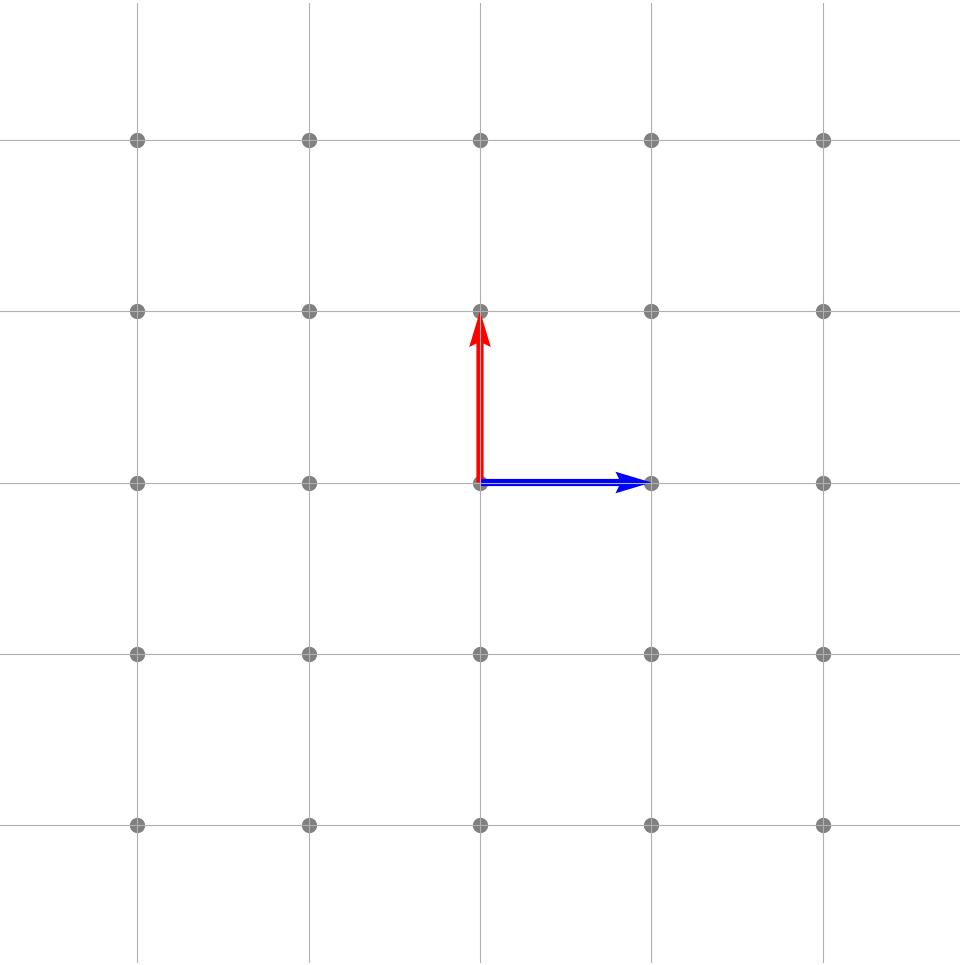
\includegraphics[width=\linewidth]{zn_trivial_basis.jpeg}
            \end{column}
            \begin{column}{0.3\linewidth} % Center column
                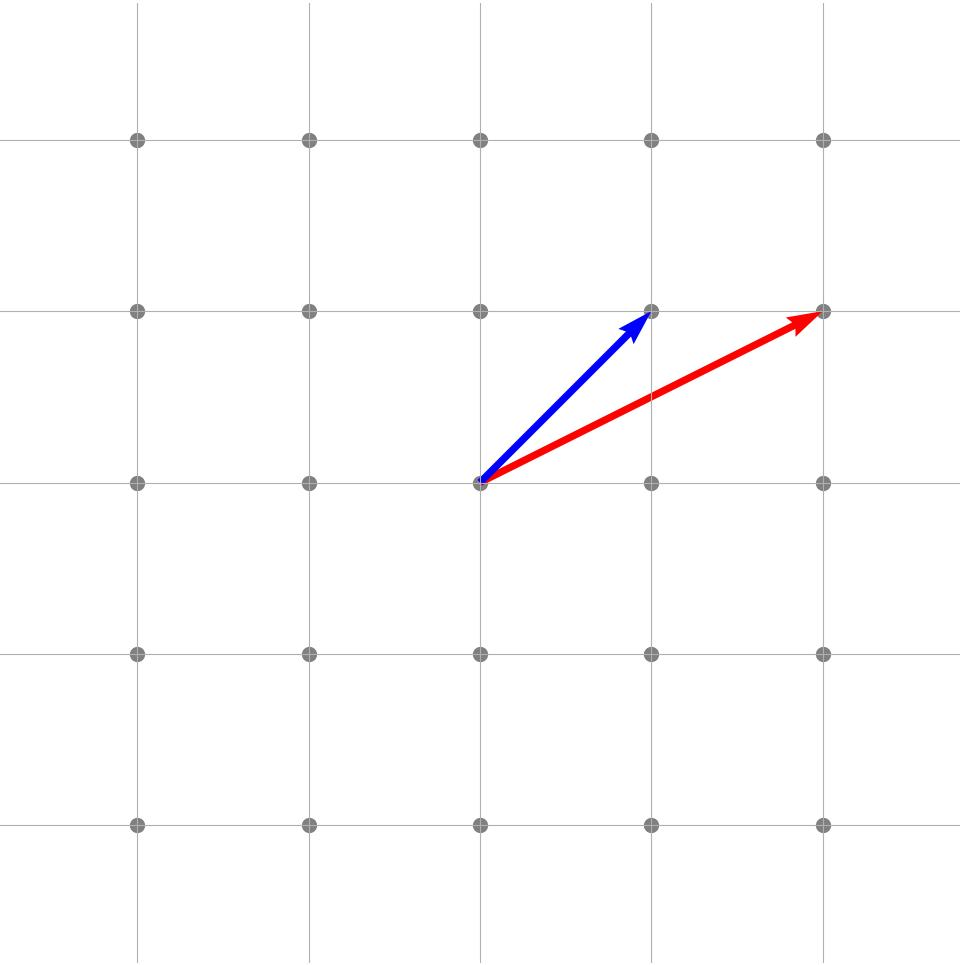
\includegraphics[width=\linewidth]{zn_nontrivial_basis.jpeg}
            \end{column}
            \begin{column}{0.3\linewidth} % Right column
                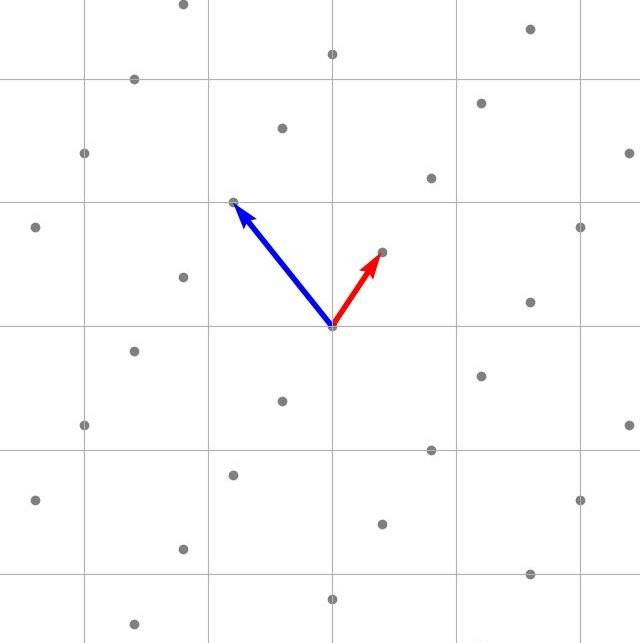
\includegraphics[width=\linewidth]{Figure_1.jpeg}
            \end{column}
        \end{columns}
    \end{adjustwidth}
\end{frame}

%------------------------------------------------

\begin{frame}
    \frametitle{What are hard lattice problems?}

    \begin{adjustwidth}{0cm}{0cm} % The first parameter is the left margin indentation and the second is the right margin indentation

        \begin{tcolorbox}[colback=ICLBlue!5!white,colframe=ICLBlue,title=\textbf{Definition:} Shortest Vector Problem (SVP)]
            Given a lattice, find the shortest \textit{non-zero} lattice point.
        \end{tcolorbox}

        \begin{tcolorbox}[colback=ICLBlue!5!white,colframe=ICLBlue,title=\textbf{Definition:} Learning With Errors Problem (LWE)]
            Let, $\color{ForestGreen} \begin{bmatrix} \\ \mathbf{b} \\ \\ \end{bmatrix} \color{black} = \color{ForestGreen} \begin{bmatrix} & & \\ & \mathbf{A} & \\ & & \end{bmatrix} \color{black} \begin{bmatrix} \\ \mathbf{s} \\ \\ \end{bmatrix} + \begin{bmatrix} \\ \mathbf{e} \\ \\ \end{bmatrix}$.
            Knowing \textit{only} the values in \color{ForestGreen} green\color{black}, find $\begin{bmatrix} \\ \mathbf{s} \\ \\ \end{bmatrix}$.
        \end{tcolorbox}
        \begin{tcolorbox}[colback=ICLBlue!5!white,colframe=ICLBlue,title=\textbf{Definition:} Lattice Isomorphism Problem (LIP)]
            Given two lattices, $\mathcal{L}_1$ and $\mathcal{L}_2$, find the scaling factor and rotation to send one to the other (if it exists).
        \end{tcolorbox}

        But we also have the Short Integer Solutions problem (SIS), the NTRU problem, the Closest Vector Problem (CVP), and all the many variants of anything mentioned here!

    \end{adjustwidth}
\end{frame}

%------------------------------------------------

\begin{frame}
    \frametitle{Shortest/Closest Vector Problem}
    \begin{columns}[T] % [T] ensures correct vertical alignment
        \begin{column}{0.48\linewidth} % Left column
            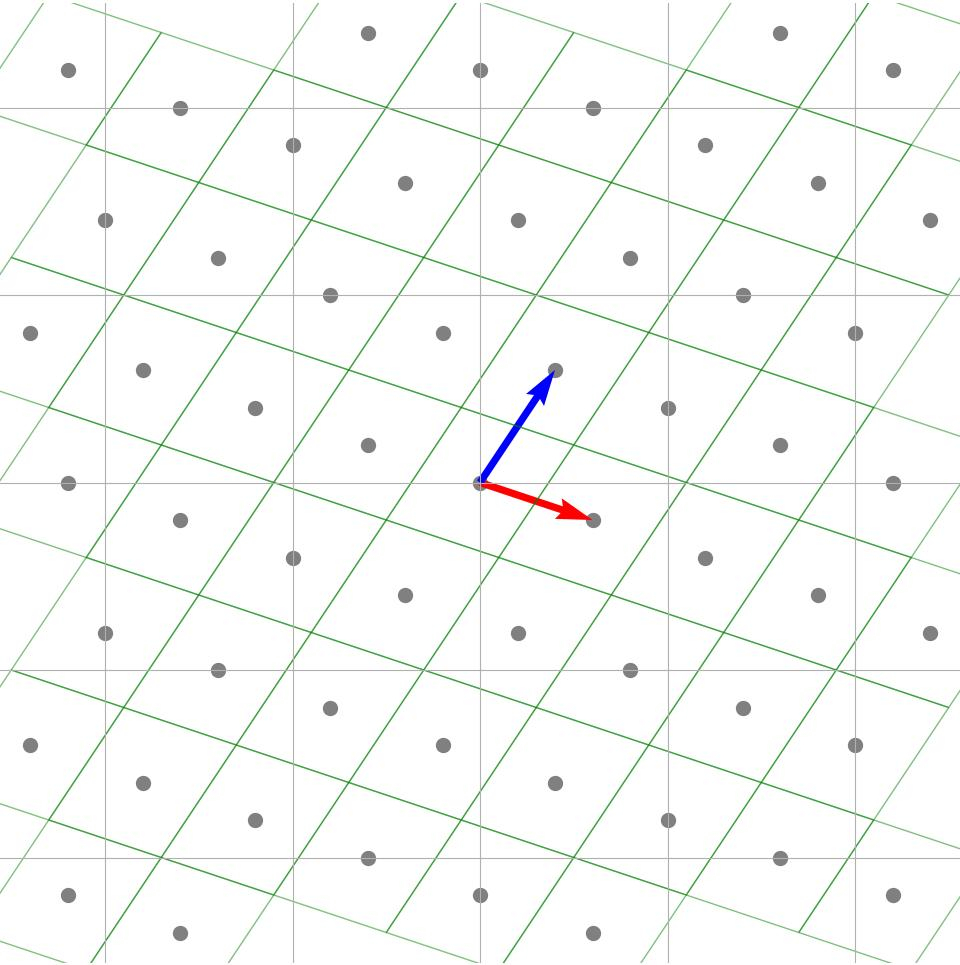
\includegraphics[width=\linewidth]{good_basis_svp.jpeg} % Trimming is used to crop your image and the order of dimensions is: left, bottom, right, top. It's recommended to crop outside of LaTeX though, to ensure the aspect ratio remains the same.
        \end{column}
        \begin{column}{0.48\linewidth} % Right column
            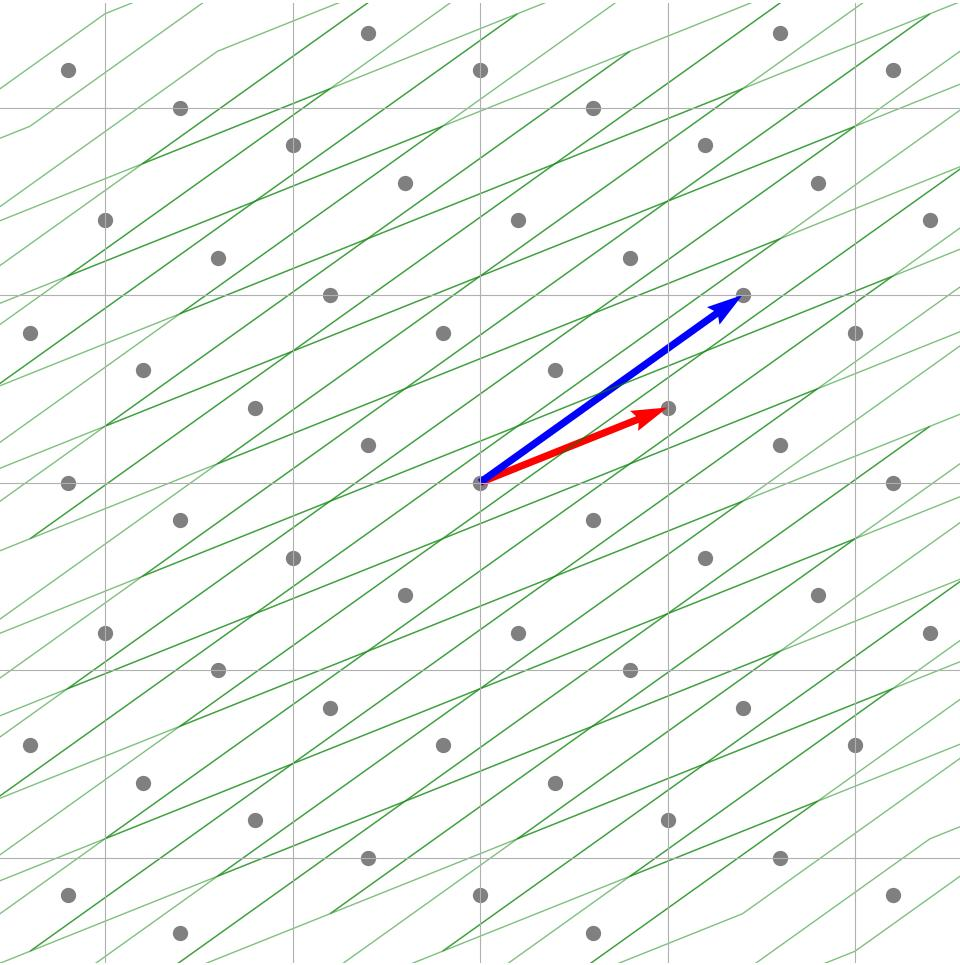
\includegraphics[width=\linewidth]{bad_basis_svp.jpeg} % Trimming is used to crop your image and the order of dimensions is: left, bottom, right, top. It's recommended to crop outside of LaTeX though, to ensure the aspect ratio remains the same.
            {\tiny\textcolor{ICLBlue}{(Above) Cryptographers wanting new toys, circa 2000 (colourised)}}
        \end{column}
    \end{columns}
\end{frame}

%------------------------------------------------

\begin{frame}
    \frametitle{It's all SVP?}

    \begin{columns}[T] % [T] ensures correct vertical alignment
        \begin{column}{0.58\linewidth} % Left column
            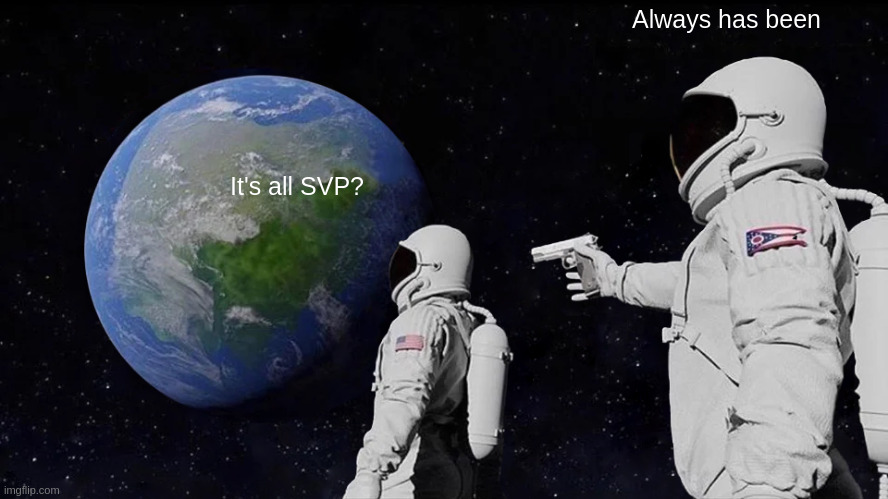
\includegraphics[width=0.9\linewidth]{always_has_been.jpg} % Trimming is used to crop your image and the order of dimensions is: left, bottom, right, top. It's recommended to crop outside of LaTeX though, to ensure the aspect ratio remains the same.

            \vspace{-1.5em}{\tiny\textcolor{ICLBlue}{(Above) Regev discovering the the LWE to $\gamma$-SVP reduction, 2005}}\newline

            \vspace{-2em}But don't worry, even though all of these problems are reducible to SVP, they all work in slightly different ways, giving the schemes we build from them different properties (speed, key size, etc.) We also believe that SVP is a \textit{very} hard problem, even for quantum computers.
        \end{column}
        \begin{column}{0.38\linewidth} % Right column
            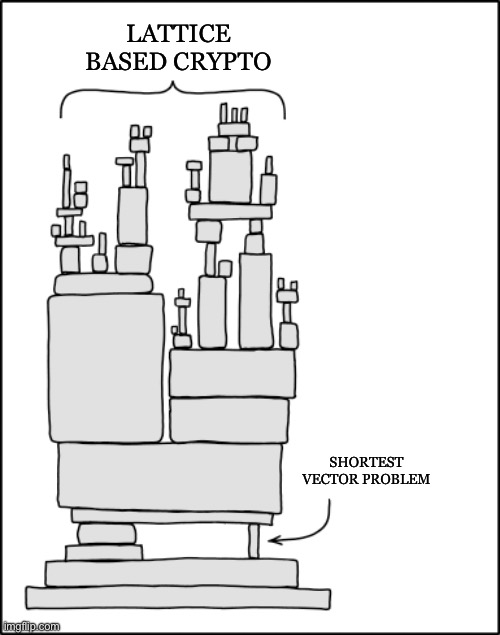
\includegraphics[width=0.85\linewidth]{svp_crutch.jpeg} % Trimming is used to crop your image and the order of dimensions is: left, bottom, right, top. It's recommended to crop outside of LaTeX though, to ensure the aspect ratio remains the same.

            \vspace{-1.5em}{\tiny\textcolor{ICLBlue}{(Above) xkcd Dependency, lattice based cryptography special edition}}
        \end{column}
    \end{columns}
\end{frame}

%------------------------------------------------

\begin{frame}
    \frametitle{Slide Title}
    \framesubtitle{Section Title Examples}

    \begin{columns}[T] % [T] ensures correct vertical alignment
        \begin{column}{0.48\linewidth} % Left column
            \textbf{Section Title}\\
            Sed et mincipidem am fugia venihi aut utatem invellupis dolore voluptatiate veor mo dolendi squatur?

            Ab illate sitate explibus reiundusam, voluptur sim idebit, omnis dero quas adio quatur?

            Pa cumquat ute nos exero magnime officatem. Luptia voluptatur aut acia comnist qui beatusam, omniatecae iur alit, cus debis
        \end{column}
        \begin{column}{0.48\linewidth} % Right column
            Sed et mincipidem am fugia venihitem aut utatem invellupis dolore voluptatiate verior mo dolendi squatur?

            \textbf{Section Title}\\
            Ab illate sitate explibus reiundusam, voluptur sim idebit, omnis dero quas adio quatur?

            Pa cumquat ute nos exero magnime officatem. Luptia voluptatur aut acia comnist qui beatusam, omniatecae iur alit, cus debis
        \end{column}
    \end{columns}
\end{frame}

%------------------------------------------------

\begin{frame}
    \frametitle{Slide Title}
    \framesubtitle{List Examples}

    \begin{columns}[T] % [T] ensures correct vertical alignment
        \begin{column}{0.48\linewidth} % Left column
            \textbf{Bullet List}\\
            \begin{itemize}
                \item Sed et mincipidem am fugia venihi aut utatem invellupis dolore voluptatiate veor mo dolendi squatur?
                \item Ab illate sitate explibus reiundusam, voluptur sim idebit, omnis dero quas adio quatur?
                    \begin{itemize}
                        \item Second level indented list item.
                            \begin{itemize}
                                \item Third level indented list item.
                            \end{itemize}
                    \end{itemize}
                \item Pa cumquat ute nos exero magnime officatem. Luptia voluptatur aut acia comnist qui beatusam, omniatecae iur alit, cus debis
            \end{itemize}
        \end{column}
        \begin{column}{0.48\linewidth} % Right column
            \textbf{Numbered List}\\
            \begin{enumerate}
                \item Sed et mincipidem am fugia venihitem aut utatem invellupis dolore voluptatiate verior mo dolendi squatur?		
                \item Ab illate sitate explibus reiundusam, voluptur sim idebit, omnis dero quas adio quatur?
                    \begin{enumerate}
                        \item Second level indented list item.
                            \begin{enumerate}
                                \item Third level indented list item.
                            \end{enumerate}
                    \end{enumerate}
                \item Pa cumquat ute nos exero magnime officatem. Luptia voluptatur aut acia comnist qui beatusam, omniatecae iur alit, cus debis
            \end{enumerate}
        \end{column}
    \end{columns}
\end{frame}

%------------------------------------------------

\begin{frame}
    \frametitle{Slide Title}
    \framesubtitle{Three-Column Example}

    \small % Reduce font size in this slide

    \begin{columns}[T] % [T] ensures correct vertical alignment
        \begin{column}{0.3\linewidth} % Left column
            \textbf{Section Title}\\
            Sed et mincipidem am fugia ve nihi aut utatem invellupis dore voluptatiate veor olendi squatur?

            Ab illate sitate explibus reiundusam, voluptur sim idebit, omnis dero quas adio quatur? Pa cumquat ute nos exero magnime officatem. Luptia
        \end{column}
        \begin{column}{0.3\linewidth} % Center column
            \textbf{Section Title}\\
            Sed et mincipidem am fugia ve nihi aut utatem invellupis dore voluptatiate veor olendi squatur?

            Ab illate sitate explibus reiundusam, voluptur sim idebit, omnis dero quas adio quatur? Pa cumquat ute nos exero magnime officatem. Luptia
        \end{column}
        \begin{column}{0.3\linewidth} % Right column
            \textbf{Section Title}\\
            Sed et mincipidem am fugia ve nihi aut utatem invellupis dore voluptatiate veor olendi squatur?

            Ab illate sitate explibus reiundusam, voluptur sim idebit, omnis dero quas adio quatur? Pa cumquat ute nos exero magnime officatem. Luptia
        \end{column}
    \end{columns}
\end{frame}

%------------------------------------------------

\begin{frame}
    \frametitle{Slide Title}
    \framesubtitle{Three-Column With Images Example}

    \small % Reduce font size in this slide

    \begin{columns}[T] % [T] ensures correct vertical alignment
        \begin{column}{0.3\linewidth} % Left column
            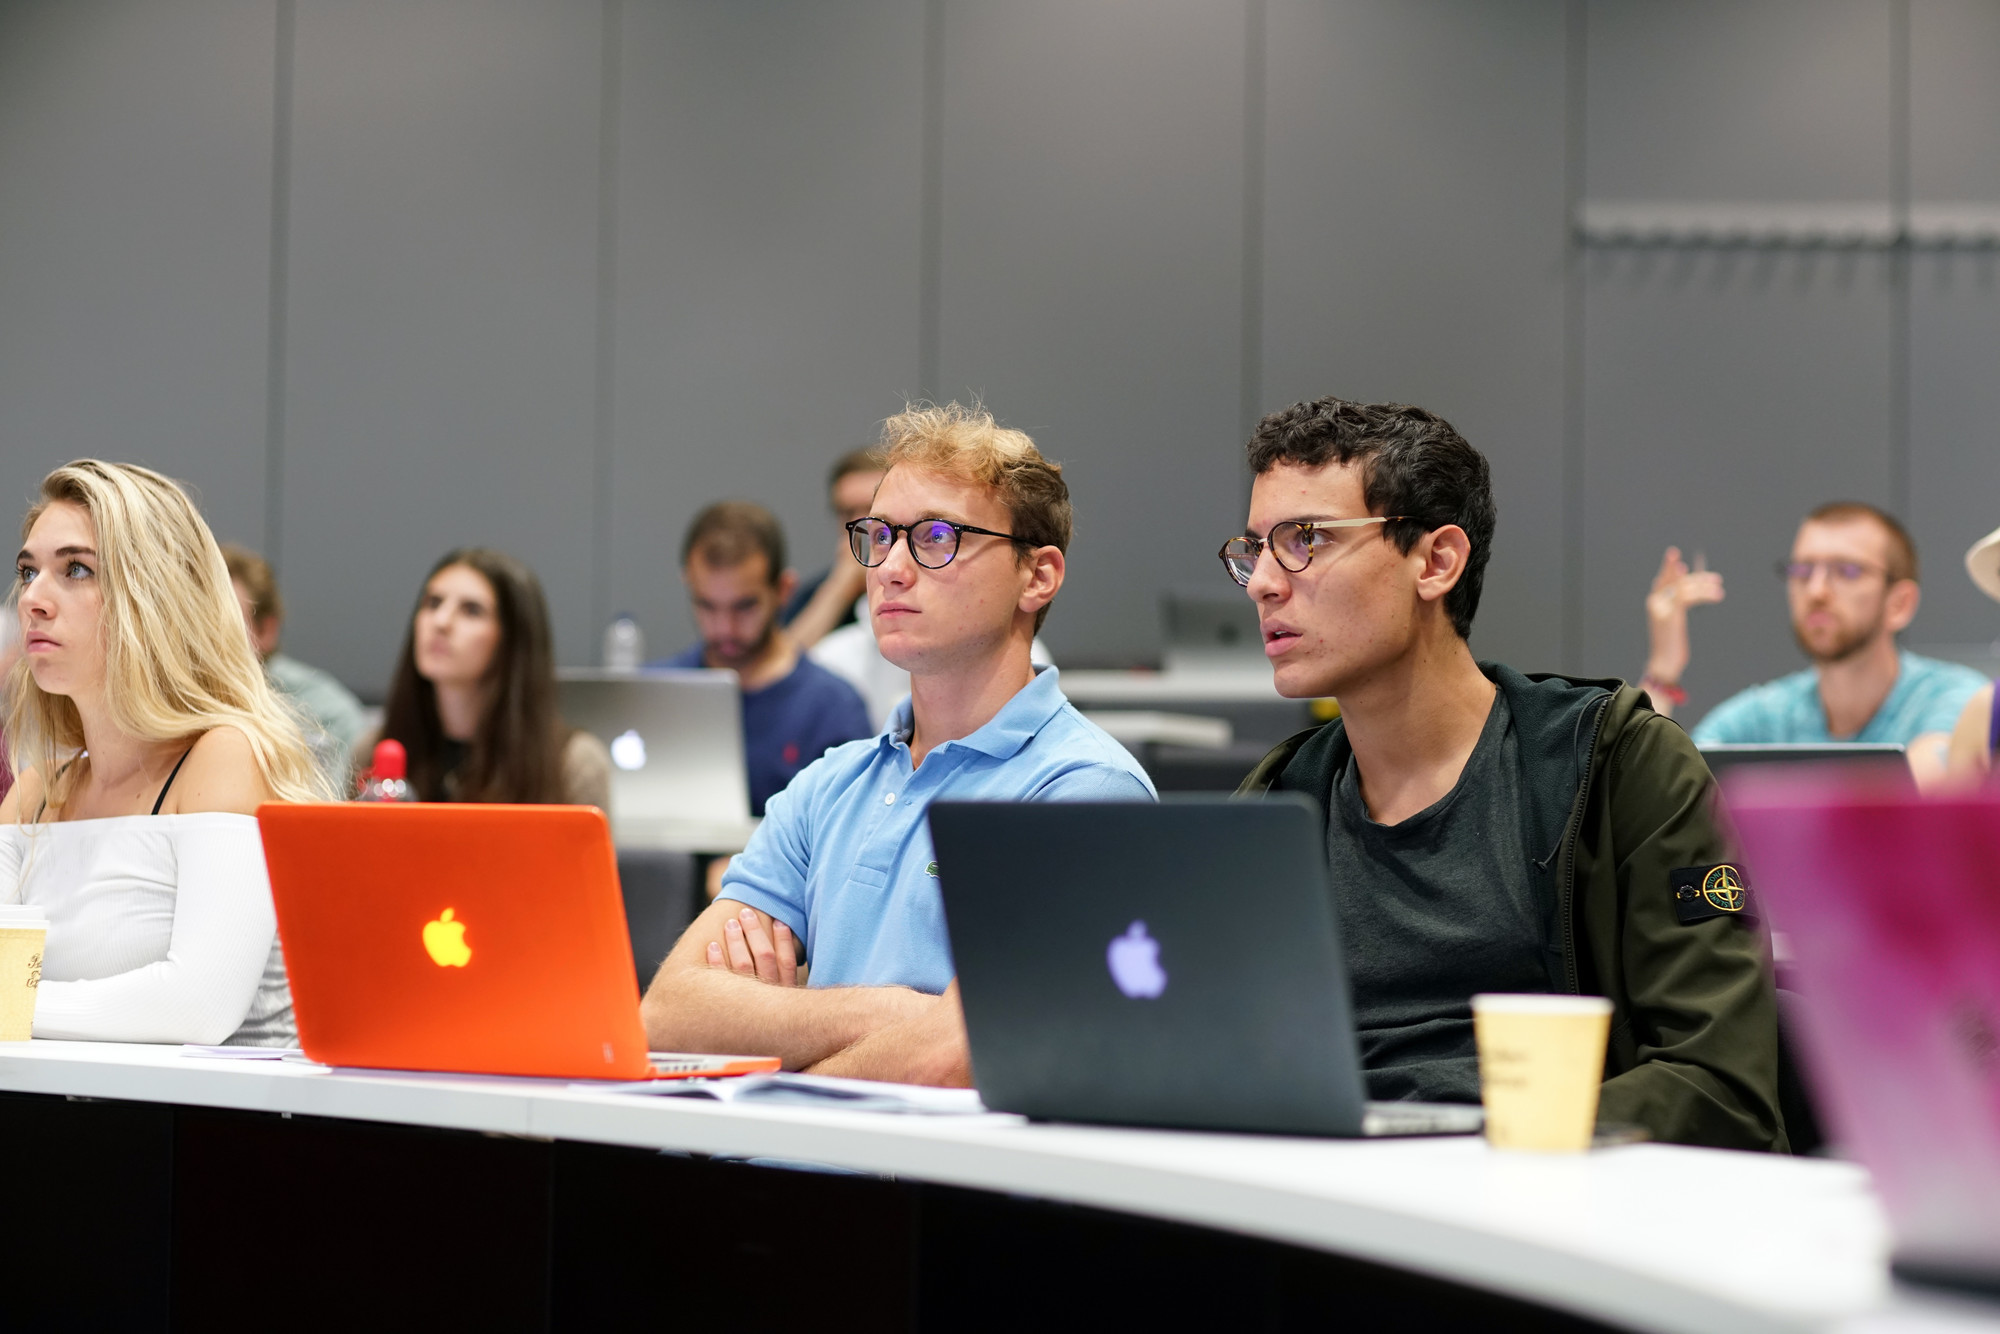
\includegraphics[width=\linewidth]{abt_7295054328859831271Mjc0ODA1Ng.jpg}\\[3pt]
            \textbf{Section Title}\\			
            Sed et mincipidem am fugia ve nihi aut utatem invellupis dore voluptatiate veor olendi squatur?

            Ab illate sitate explibus reiundusam, voluptur sim idebit?
        \end{column}
        \begin{column}{0.3\linewidth} % Center column
            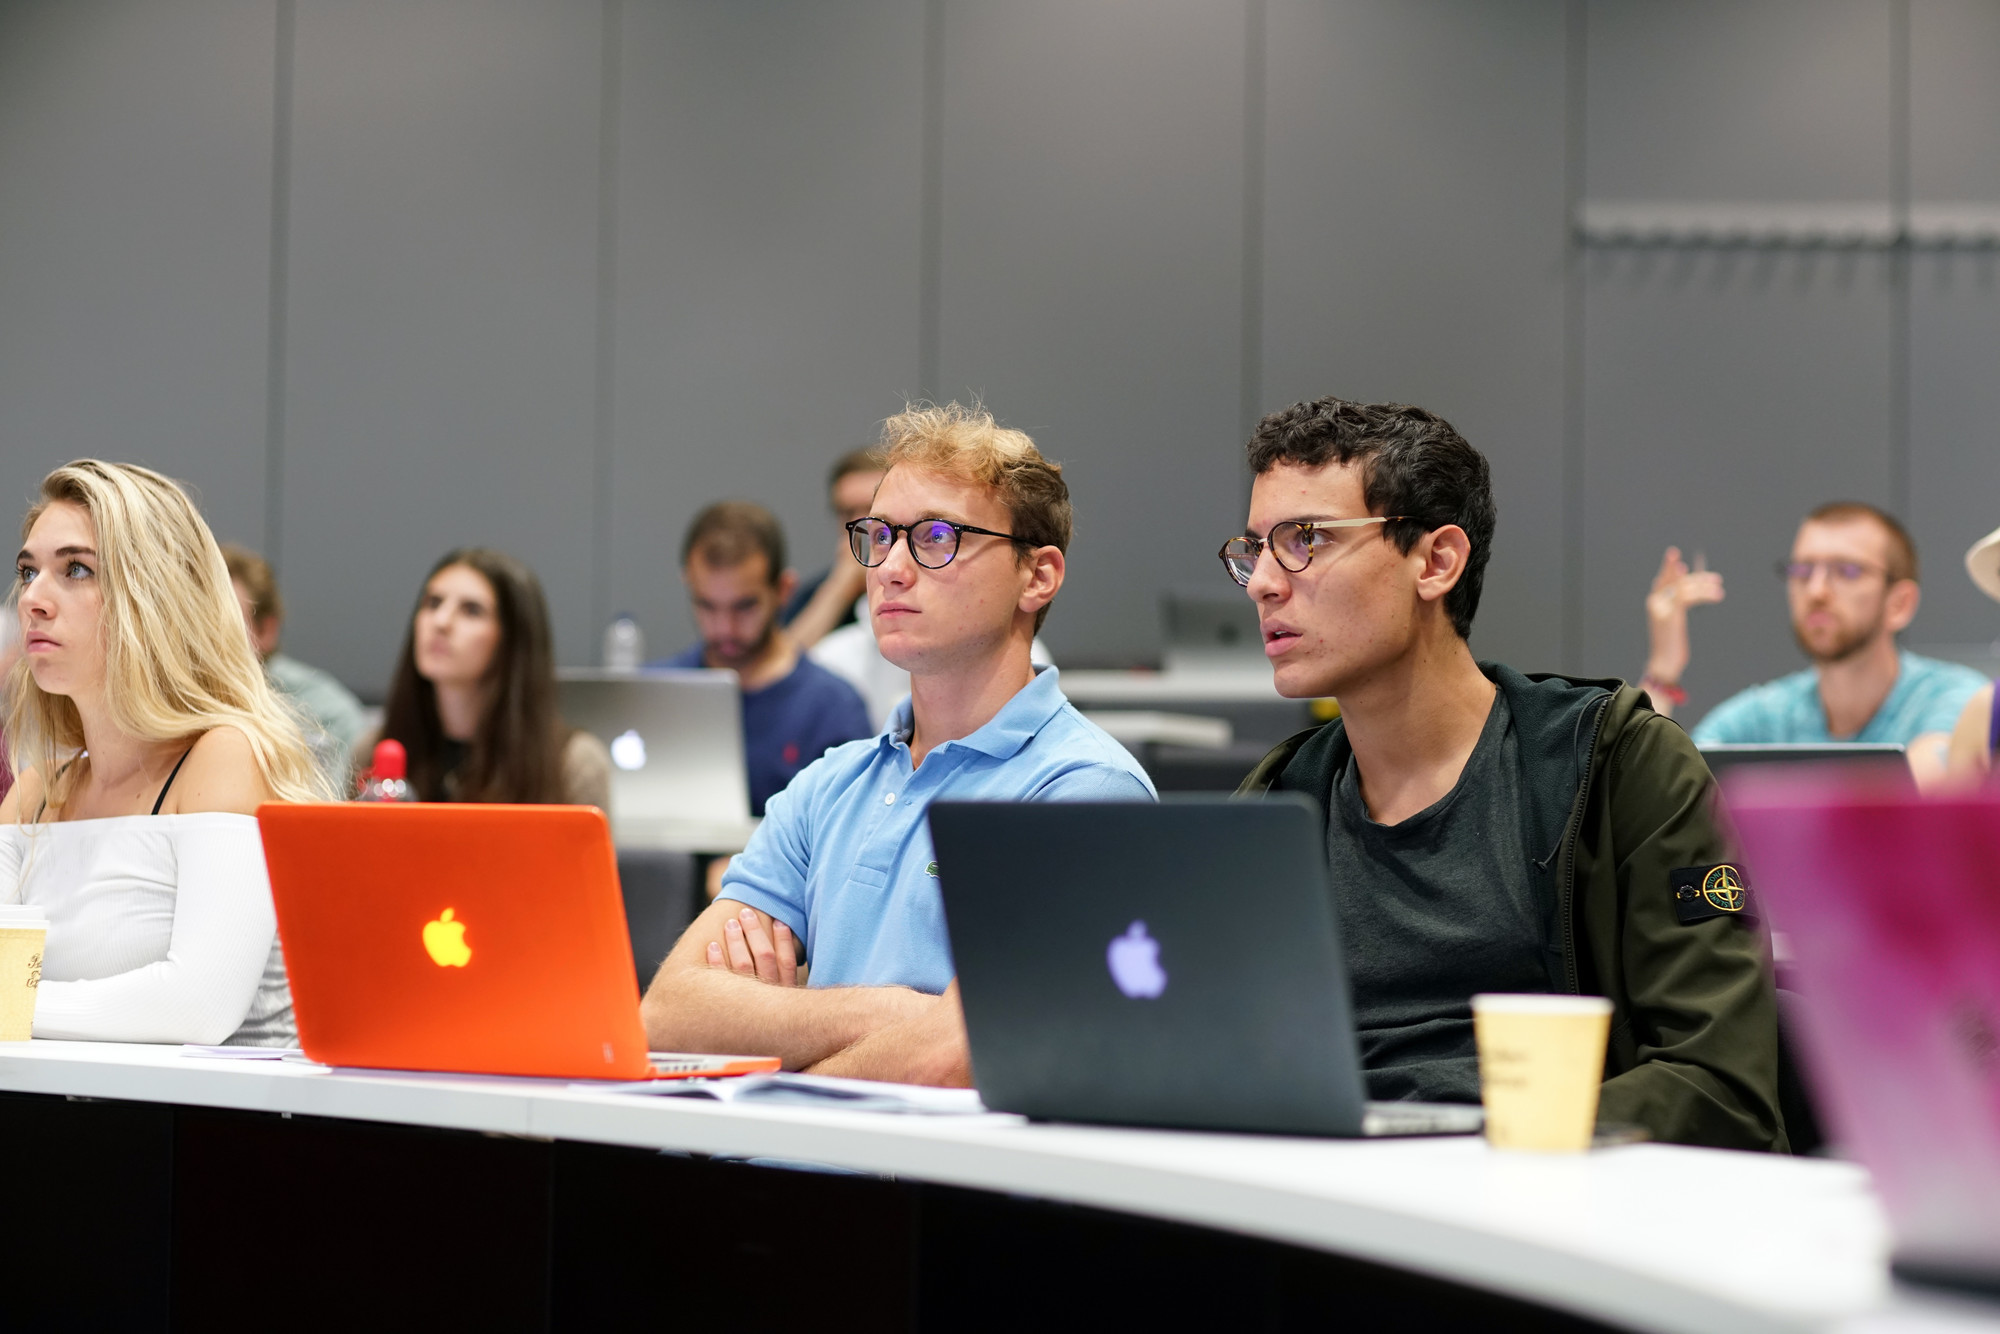
\includegraphics[width=\linewidth]{abt_7295054328859831271Mjc0ODA1Ng.jpg}\\[3pt]
            \textbf{Section Title}\\			
            Sed et mincipidem am fugia ve nihi aut utatem invellupis dore voluptatiate veor olendi squatur?

            Ab illate sitate explibus reiundusam, voluptur sim idebit?
        \end{column}
        \begin{column}{0.3\linewidth} % Right column
            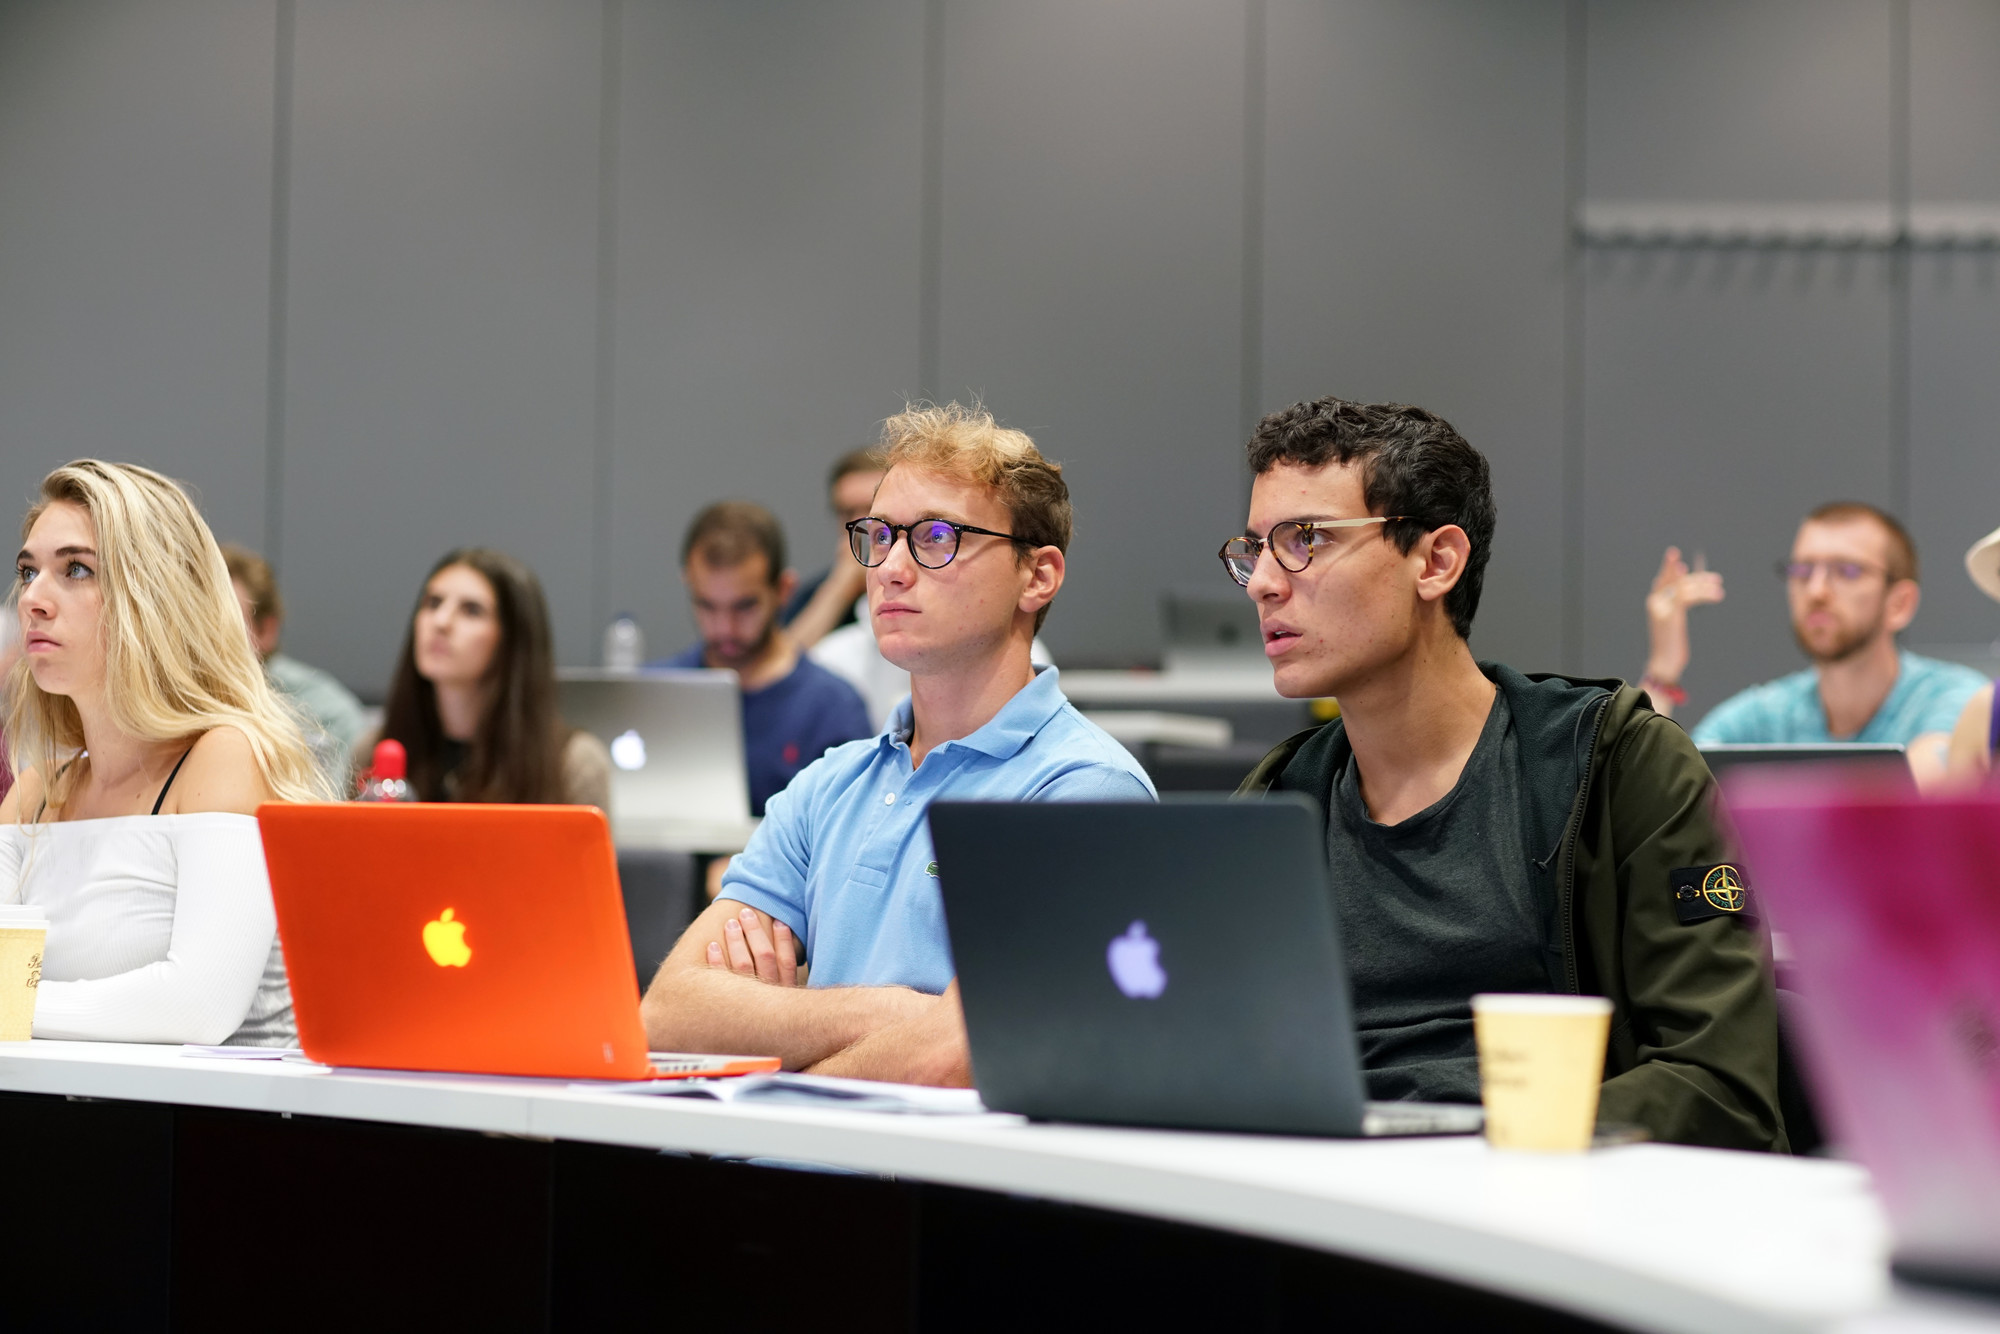
\includegraphics[width=\linewidth]{abt_7295054328859831271Mjc0ODA1Ng.jpg}\\[3pt]
            \textbf{Section Title}\\			
            Sed et mincipidem am fugia ve nihi aut utatem invellupis dore voluptatiate veor olendi squatur?

            Ab illate sitate explibus reiundusam, voluptur sim idebit?
        \end{column}
    \end{columns}
\end{frame}

%------------------------------------------------

\begin{frame}
    \frametitle{Slide Title}
    \framesubtitle{Large Right Image Example}

    \begin{columns}[T] % [T] ensures correct vertical alignment
        \begin{column}{0.48\linewidth} % Left column
            \textbf{Section Title}

            Sed et mincipidem am fugia venihi aut utatem invellupis dolore voluptatiate veor mo dolendi squatur?

            Ab illate sitate explibus reiundusam, voluptur sim idebit, omnis dero quas adio quatur?

            Pa cumquat ute nos exero magnime officatem. Luptia voluptatur aut acia comnist qui beatusam, omniatecae iur alit, cus debis
        \end{column}
        \begin{column}{0.48\linewidth} % Right column
            \vspace{-3.5\baselineskip} % Pull image up

            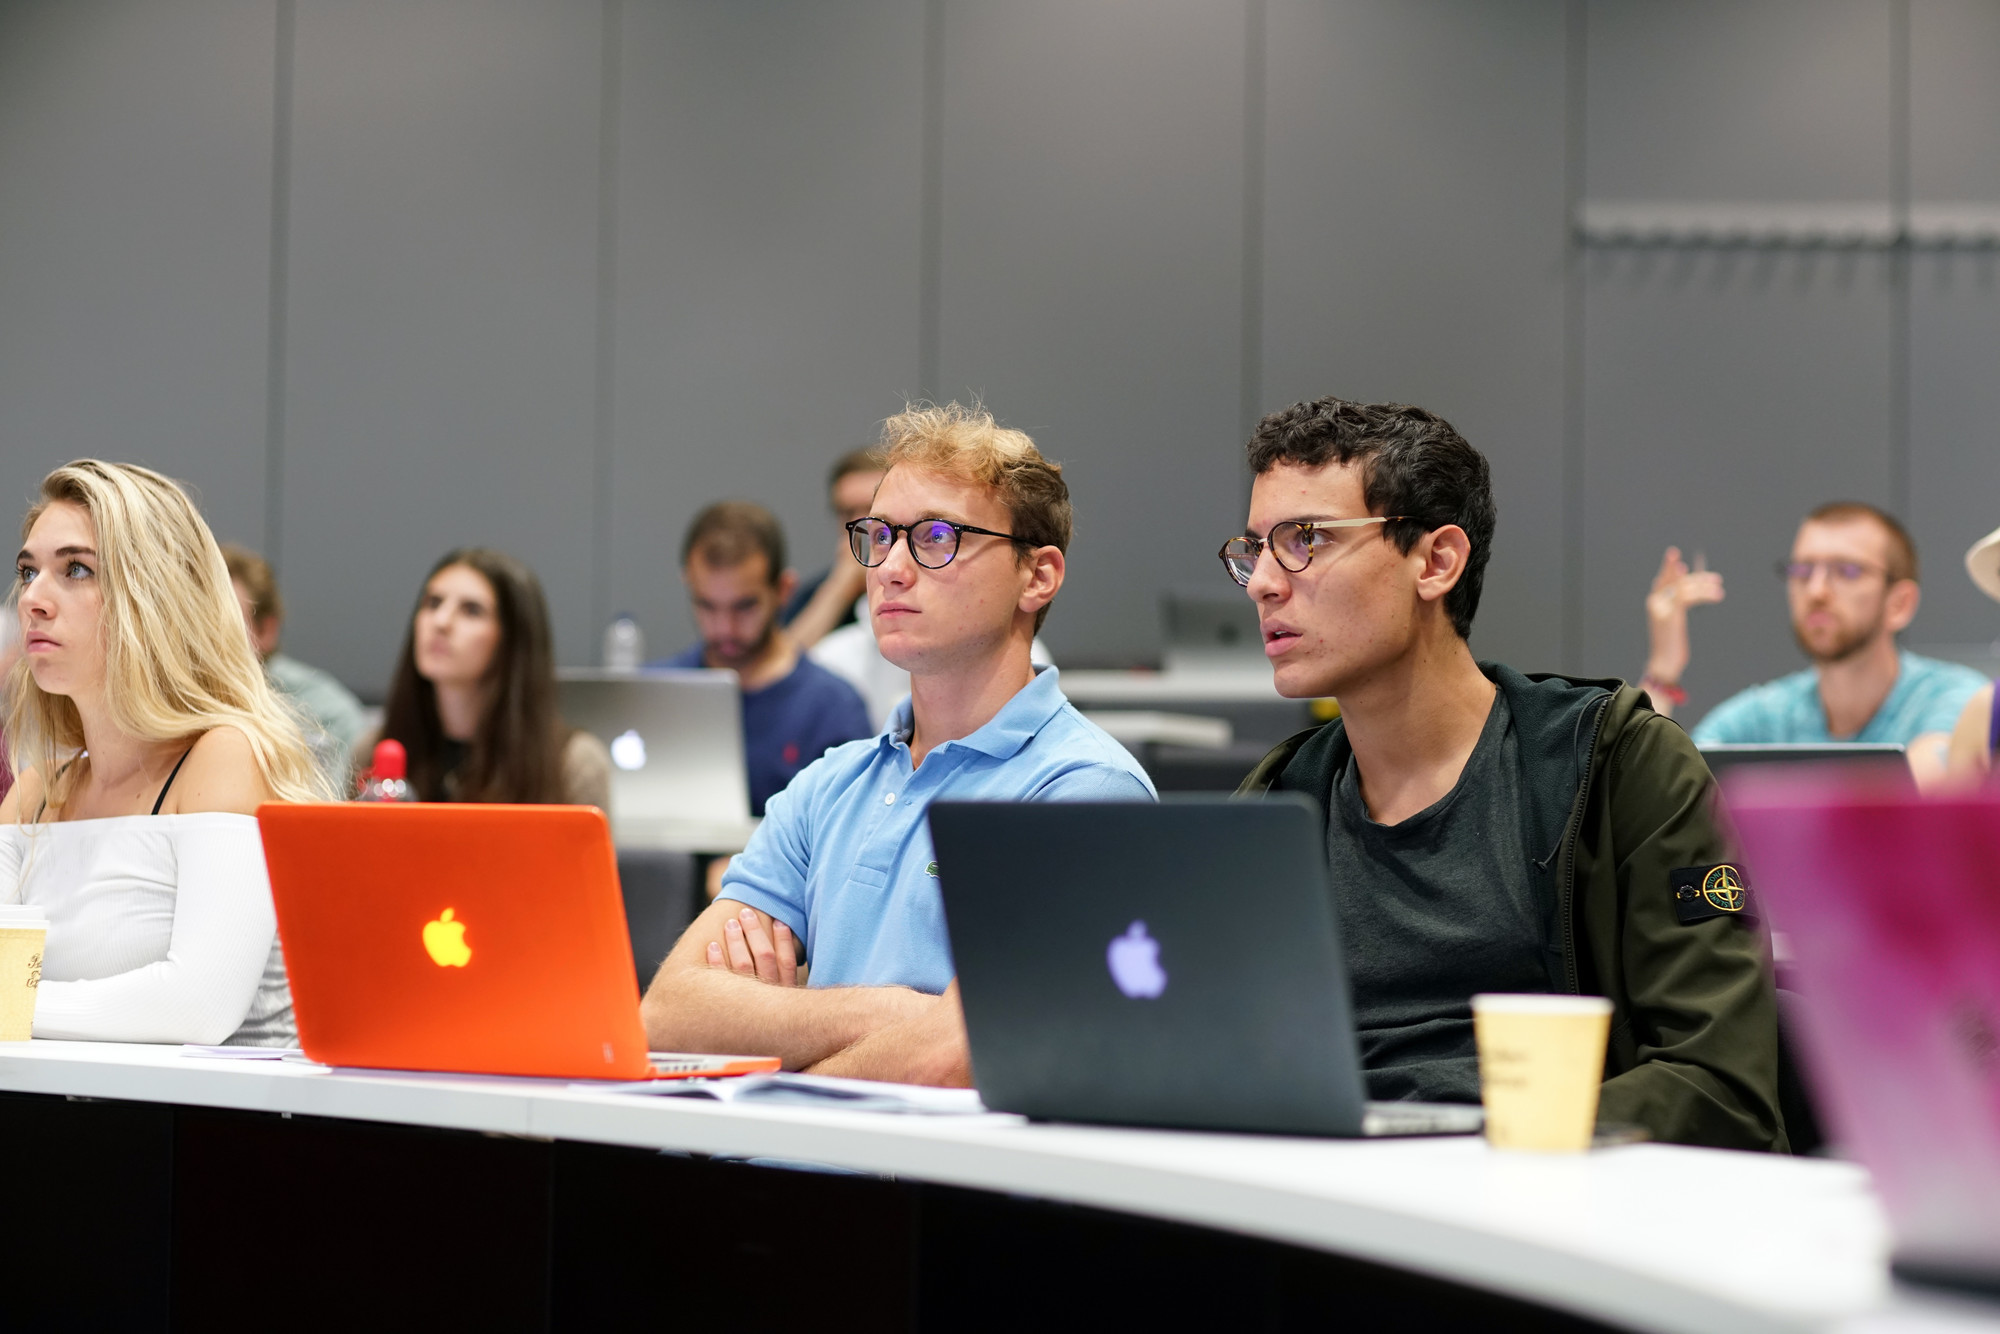
\includegraphics[trim=3cm 0cm 3cm 1cm, clip, width=\linewidth]{abt_7295054328859831271Mjc0ODA1Ng.jpg} % Trimming is used to crop your image and the order of dimensions is: left, bottom, right, top. It's recommended to crop outside of LaTeX though, to ensure the aspect ratio remains the same.
            {\tiny\textcolor{ICLBlue}{(Above) Photography Credit or Caption}}
        \end{column}
    \end{columns}
\end{frame}

%------------------------------------------------

\begin{frame}
    \begin{columns}[T] % [T] ensures correct vertical alignment
        \begin{column}{0.48\linewidth} % Left column			
            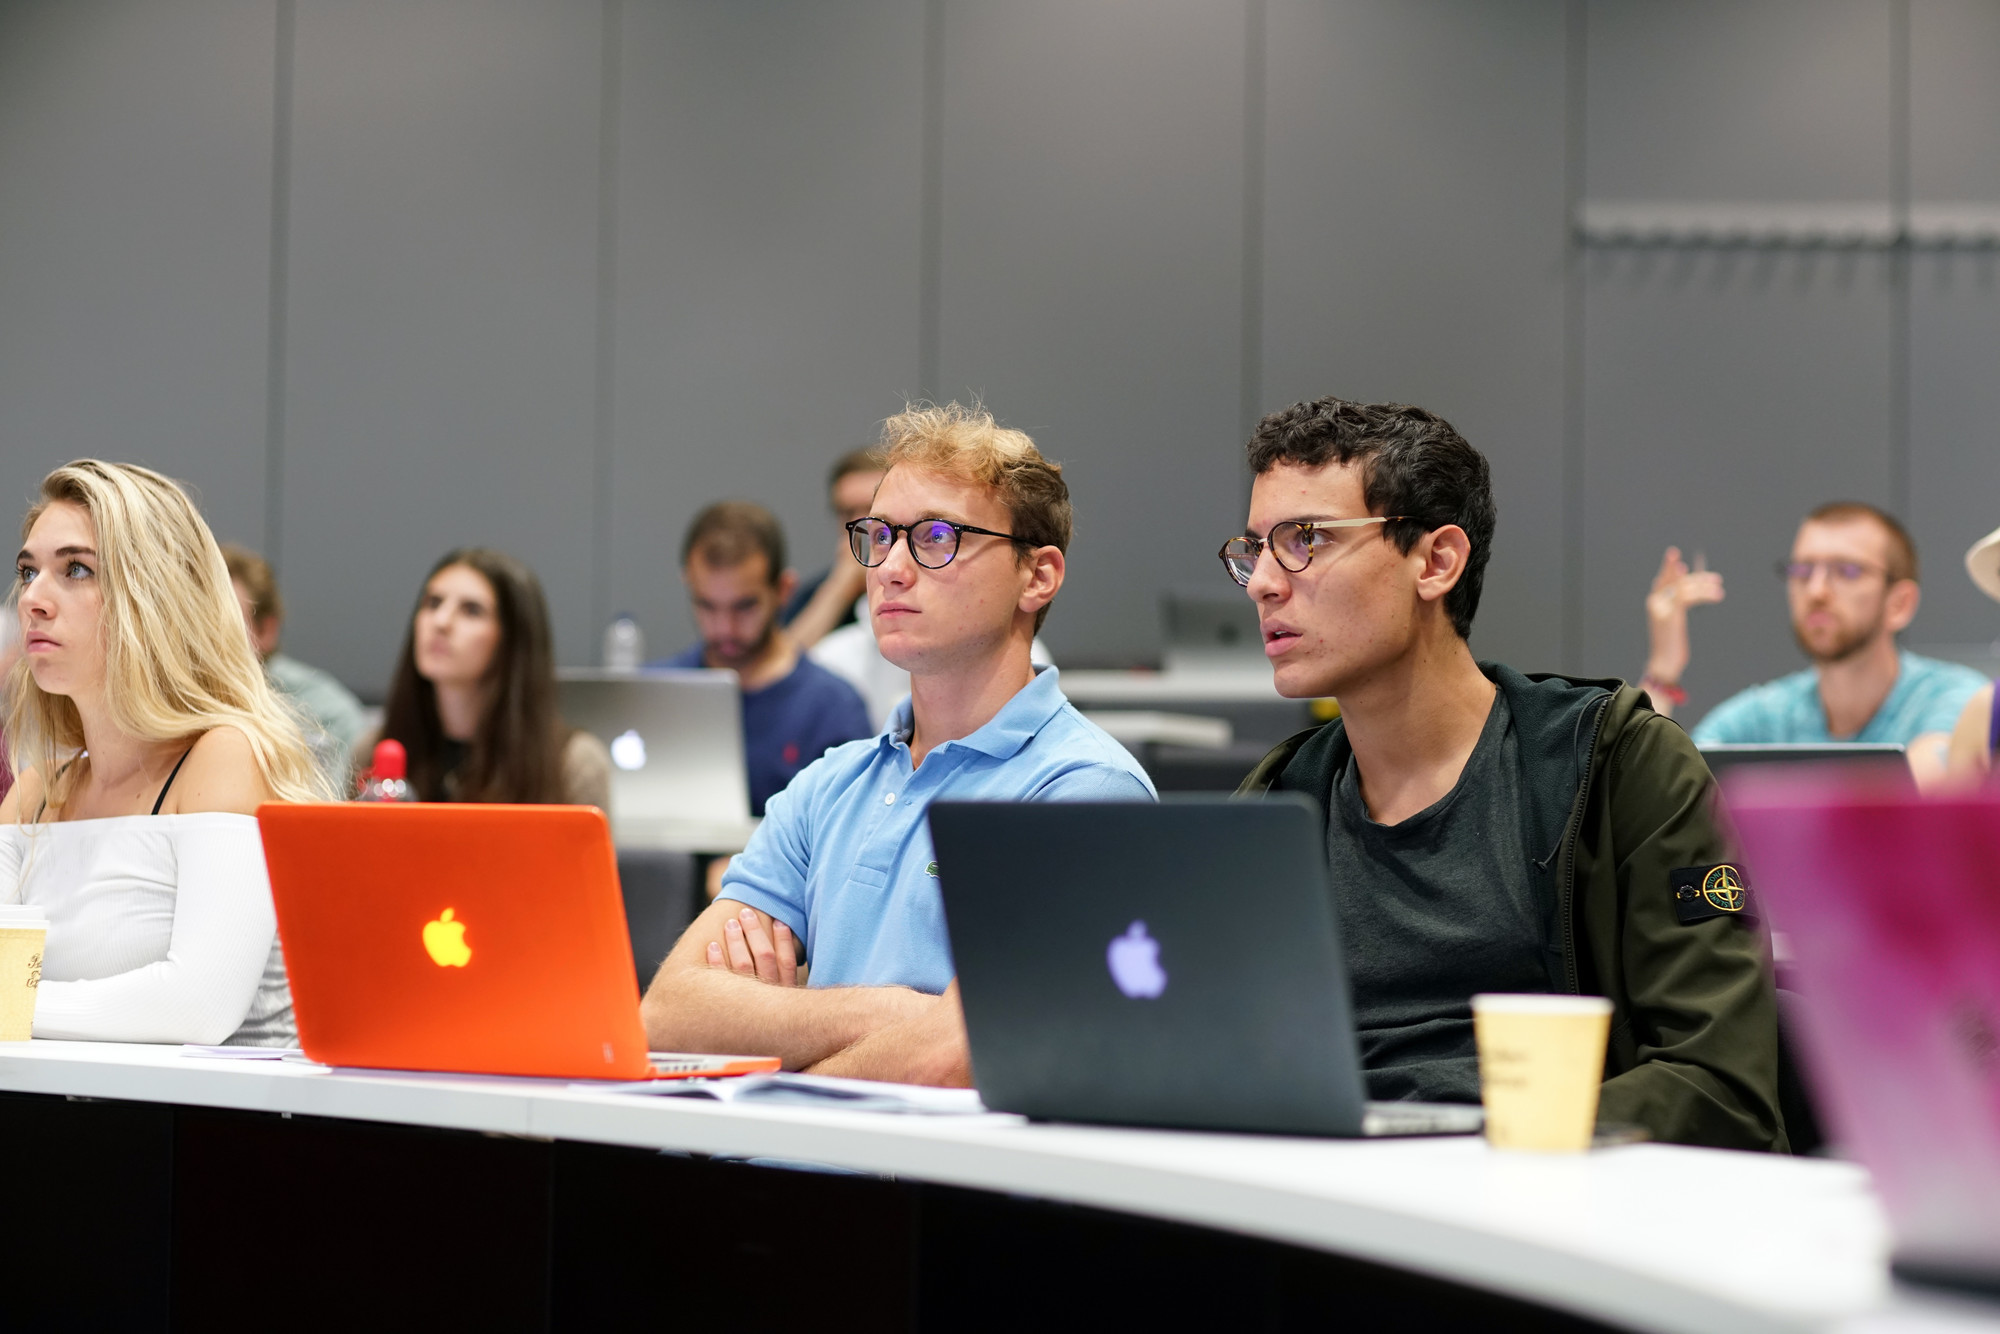
\includegraphics[trim=3cm 0cm 3cm 1cm, clip, width=\linewidth]{abt_7295054328859831271Mjc0ODA1Ng.jpg} % Trimming is used to crop your image and the order of dimensions is: left, bottom, right, top. It's recommended to crop outside of LaTeX though, to ensure the aspect ratio remains the same.
            {\tiny\textcolor{ICLBlue}{(Above) Photography Credit or Caption}}
        \end{column}
        \begin{column}{0.48\linewidth} % Right column
            \textbf{Section Title}\\
            Sed et mincipidem am fugia venihi aut utatem invellupis dolore voluptatiate veor mo dolendi squatur?

            Ab illate sitate explibus reiundusam, voluptur sim idebit, omnis dero quas adio quatur?

            Pa cumquat ute nos exero magnime officatem. Luptia voluptatur aut acia comnist qui beatusam, omniatecae iur alit, cus debis
        \end{column}
    \end{columns}
\end{frame}

%------------------------------------------------

\begin{frame}
    \begin{columns}[T] % [T] ensures correct vertical alignment
        \begin{column}{0.48\linewidth} % Left column
            \textbf{Section Title}\\
            Sed et mincipidem am fugia venihi aut utatem invellupis dolore voluptatiate veor mo dolendi squatur?

            Ab illate sitate explibus reiundusam, voluptur sim idebit, omnis dero quas adio quatur?

            Pa cumquat ute nos exero magnime officatem. Luptia voluptatur aut acia comnist qui beatusam, omniatecae iur alit, cus debis
        \end{column}
        \begin{column}{0.48\linewidth} % Right column			
            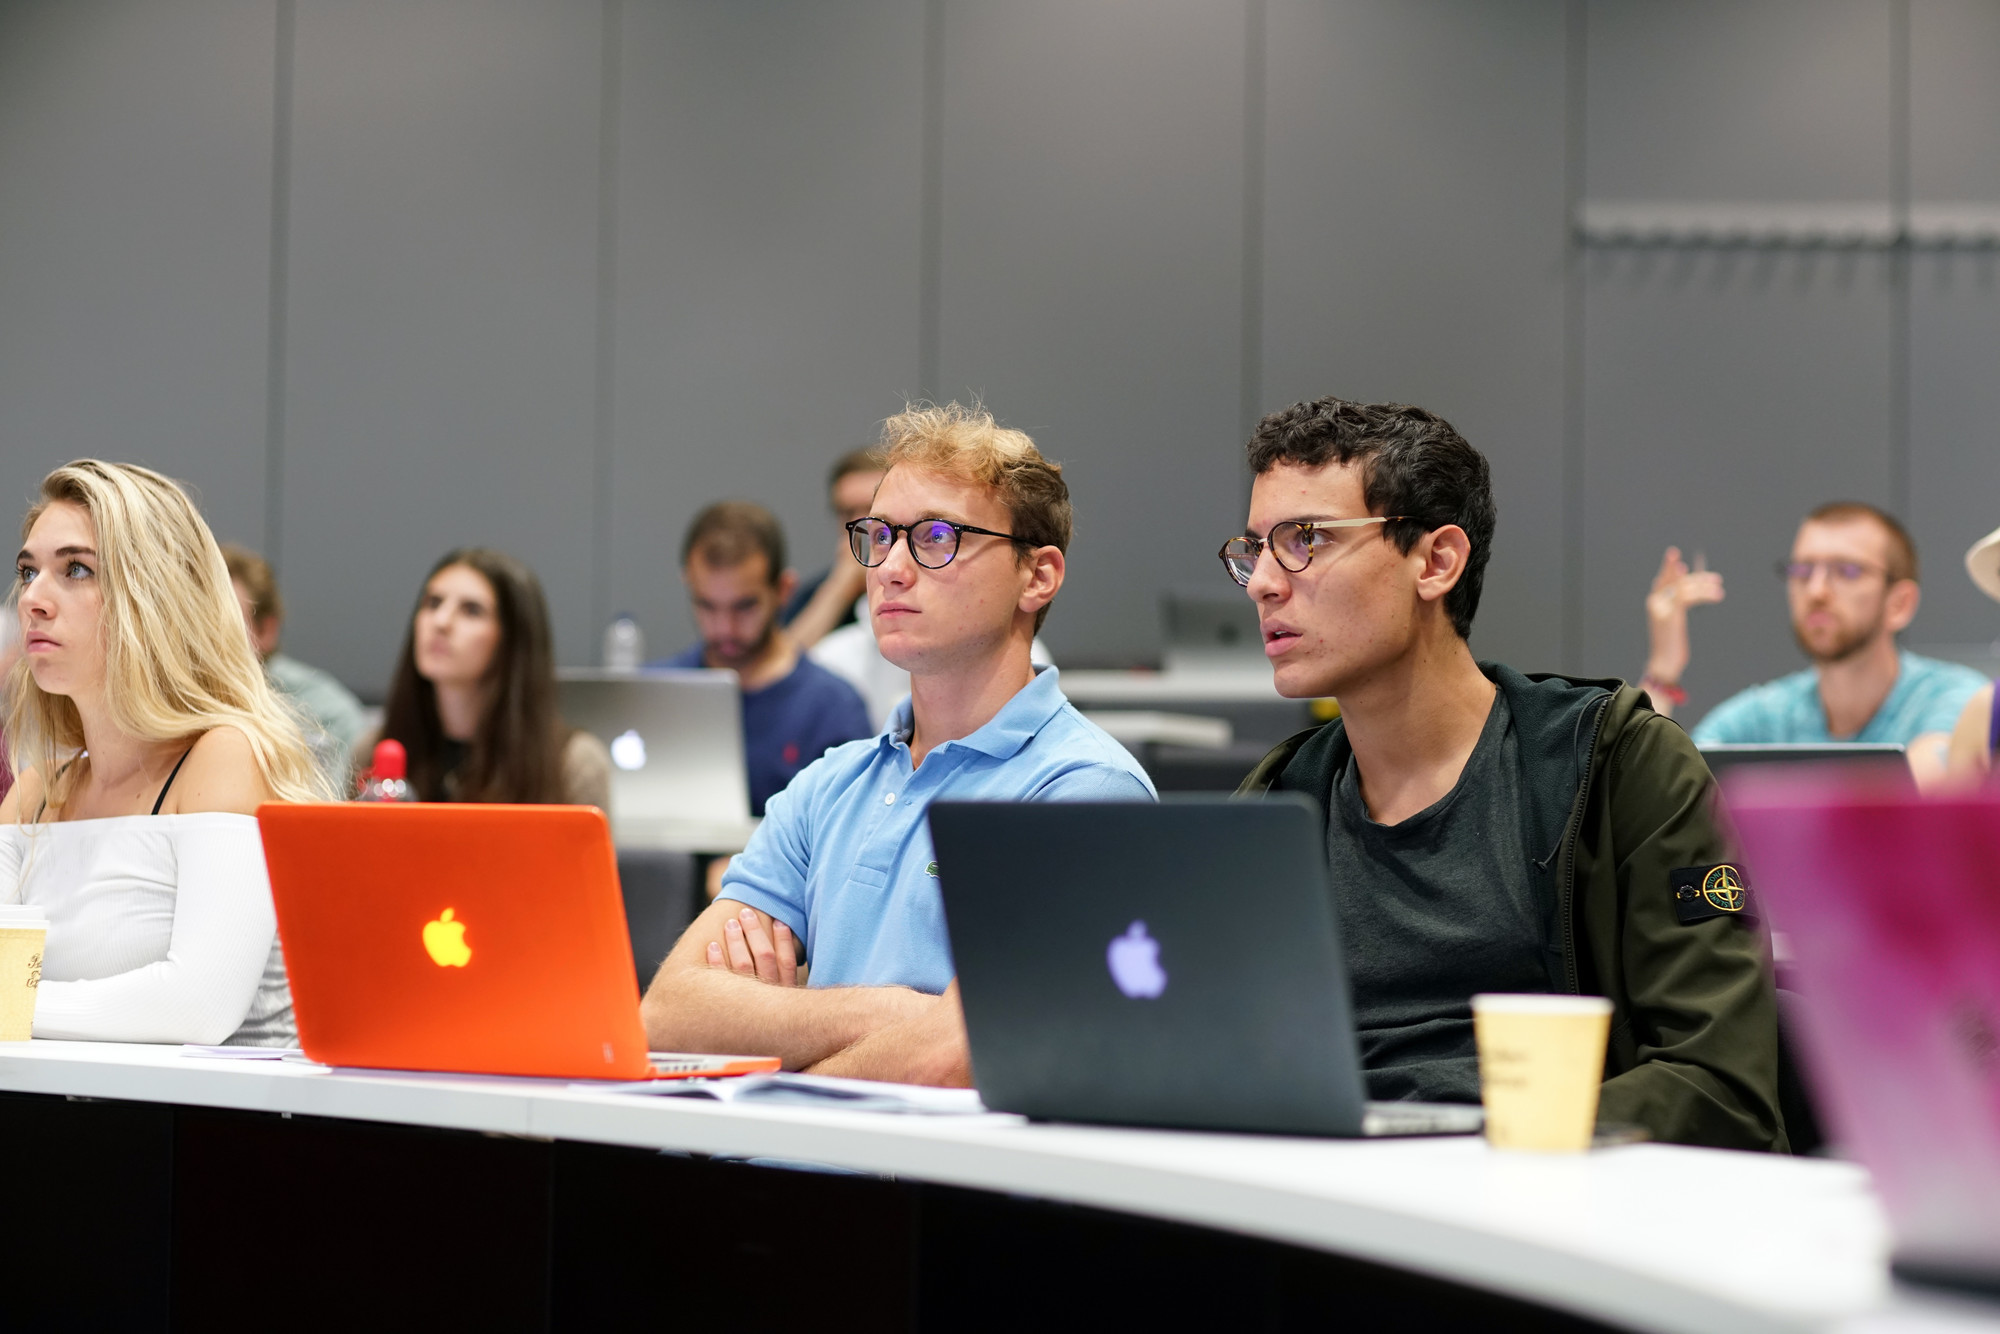
\includegraphics[trim=3cm 0cm 3cm 1cm, clip, width=\linewidth]{abt_7295054328859831271Mjc0ODA1Ng.jpg} % Trimming is used to crop your image and the order of dimensions is: left, bottom, right, top. It's recommended to crop outside of LaTeX though, to ensure the aspect ratio remains the same.
            {\tiny\textcolor{ICLBlue}{(Above) Photography Credit or Caption}}
        \end{column}
    \end{columns}
\end{frame}

%------------------------------------------------

\begin{frame}
    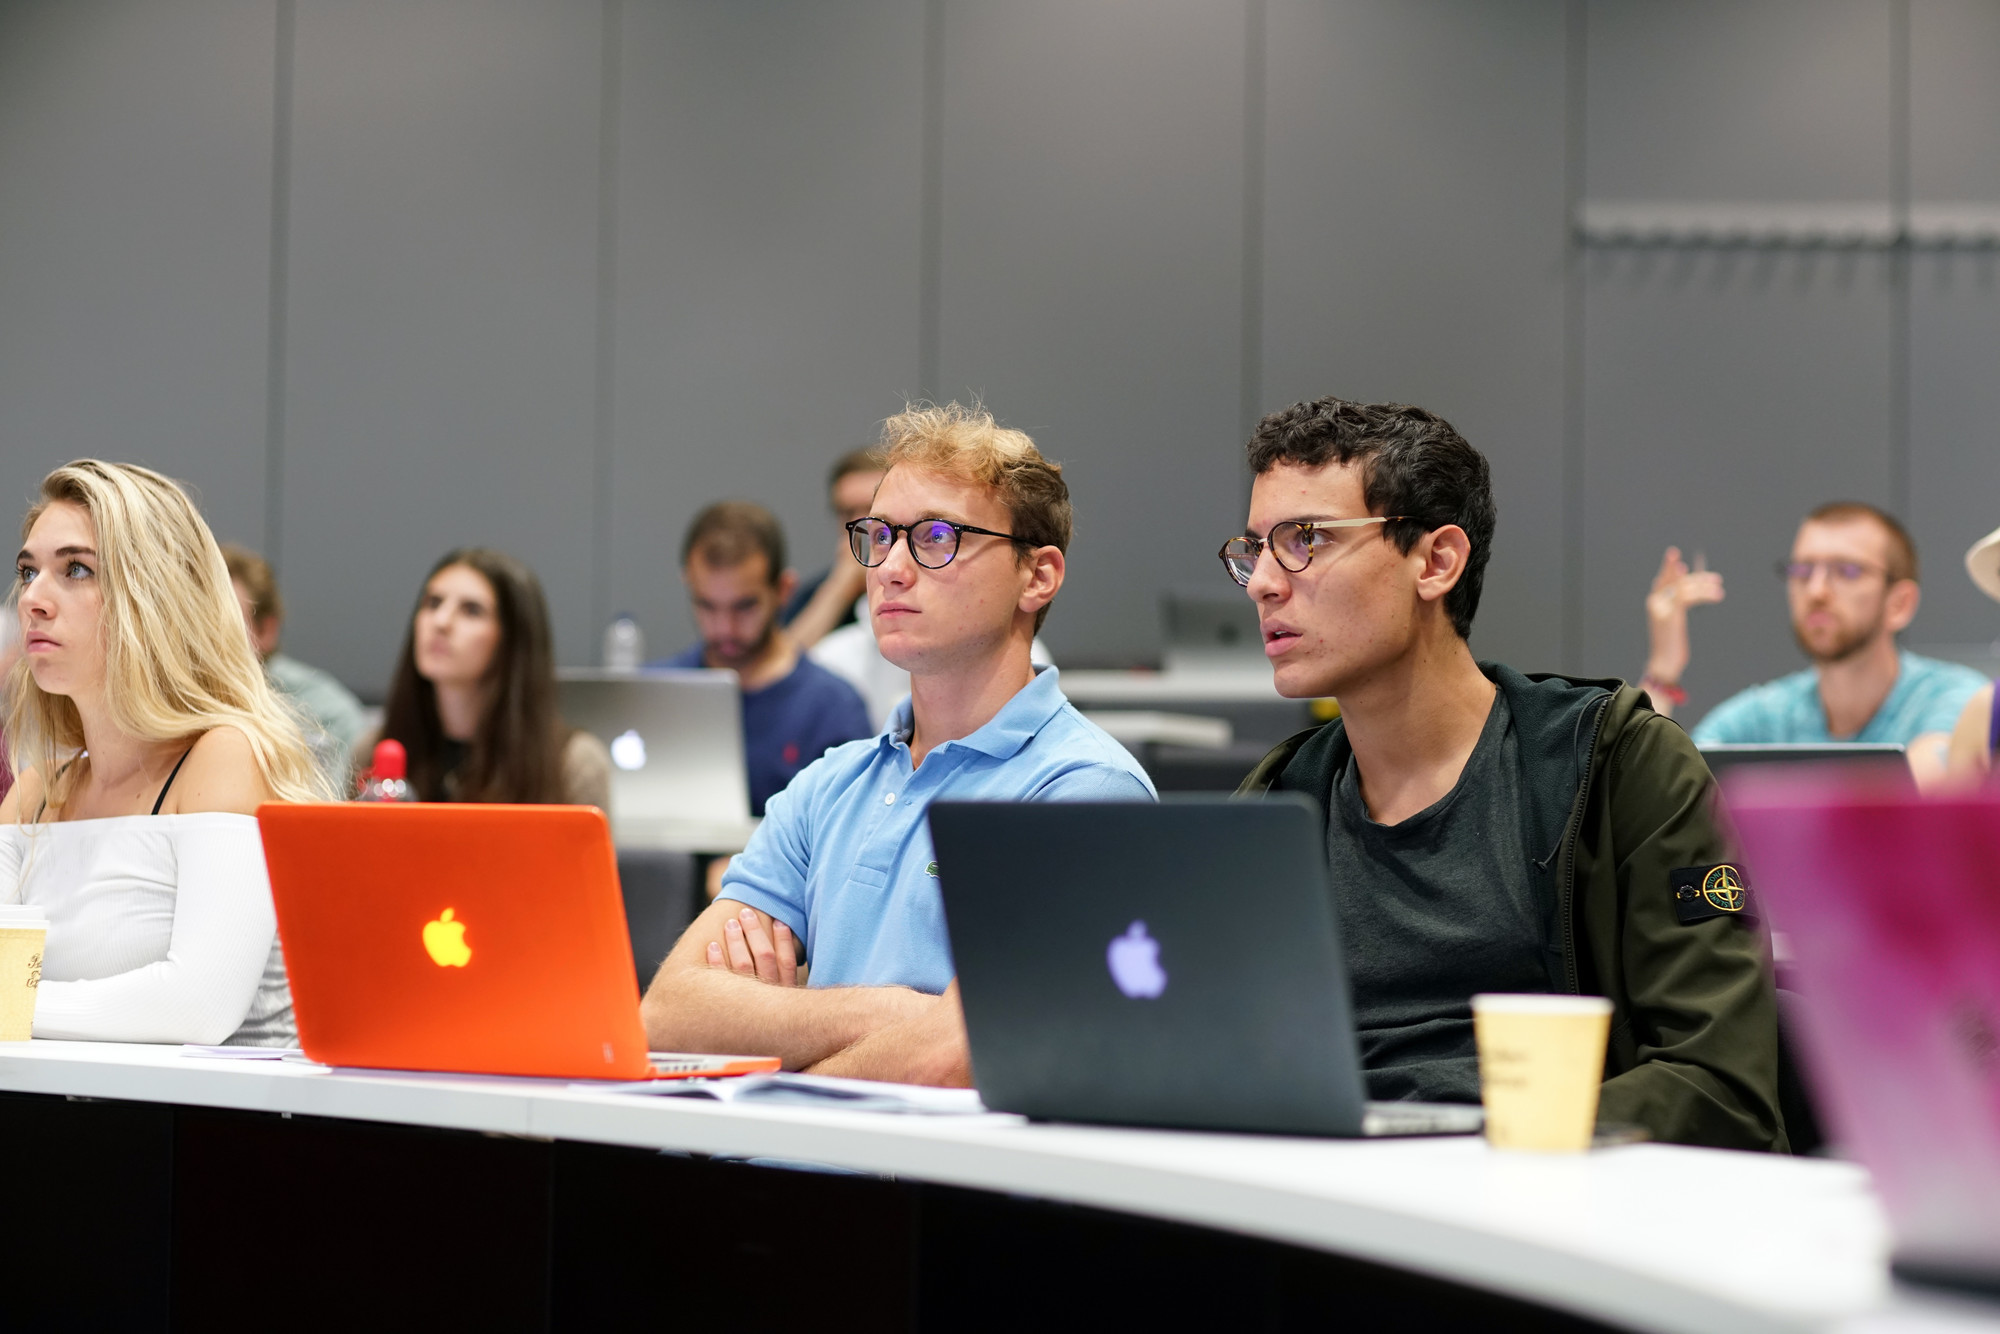
\includegraphics[trim=0cm 1.5cm 0cm 1.5cm, clip, width=\linewidth, height=\textheight]{abt_7295054328859831271Mjc0ODA1Ng.jpg} % Trimming is used to crop your image and the order of dimensions is: left, bottom, right, top. It's recommended to crop outside of LaTeX though, to ensure the aspect ratio remains the same.
\end{frame}

%------------------------------------------------

\begingroup
\setbeamertemplate{background}{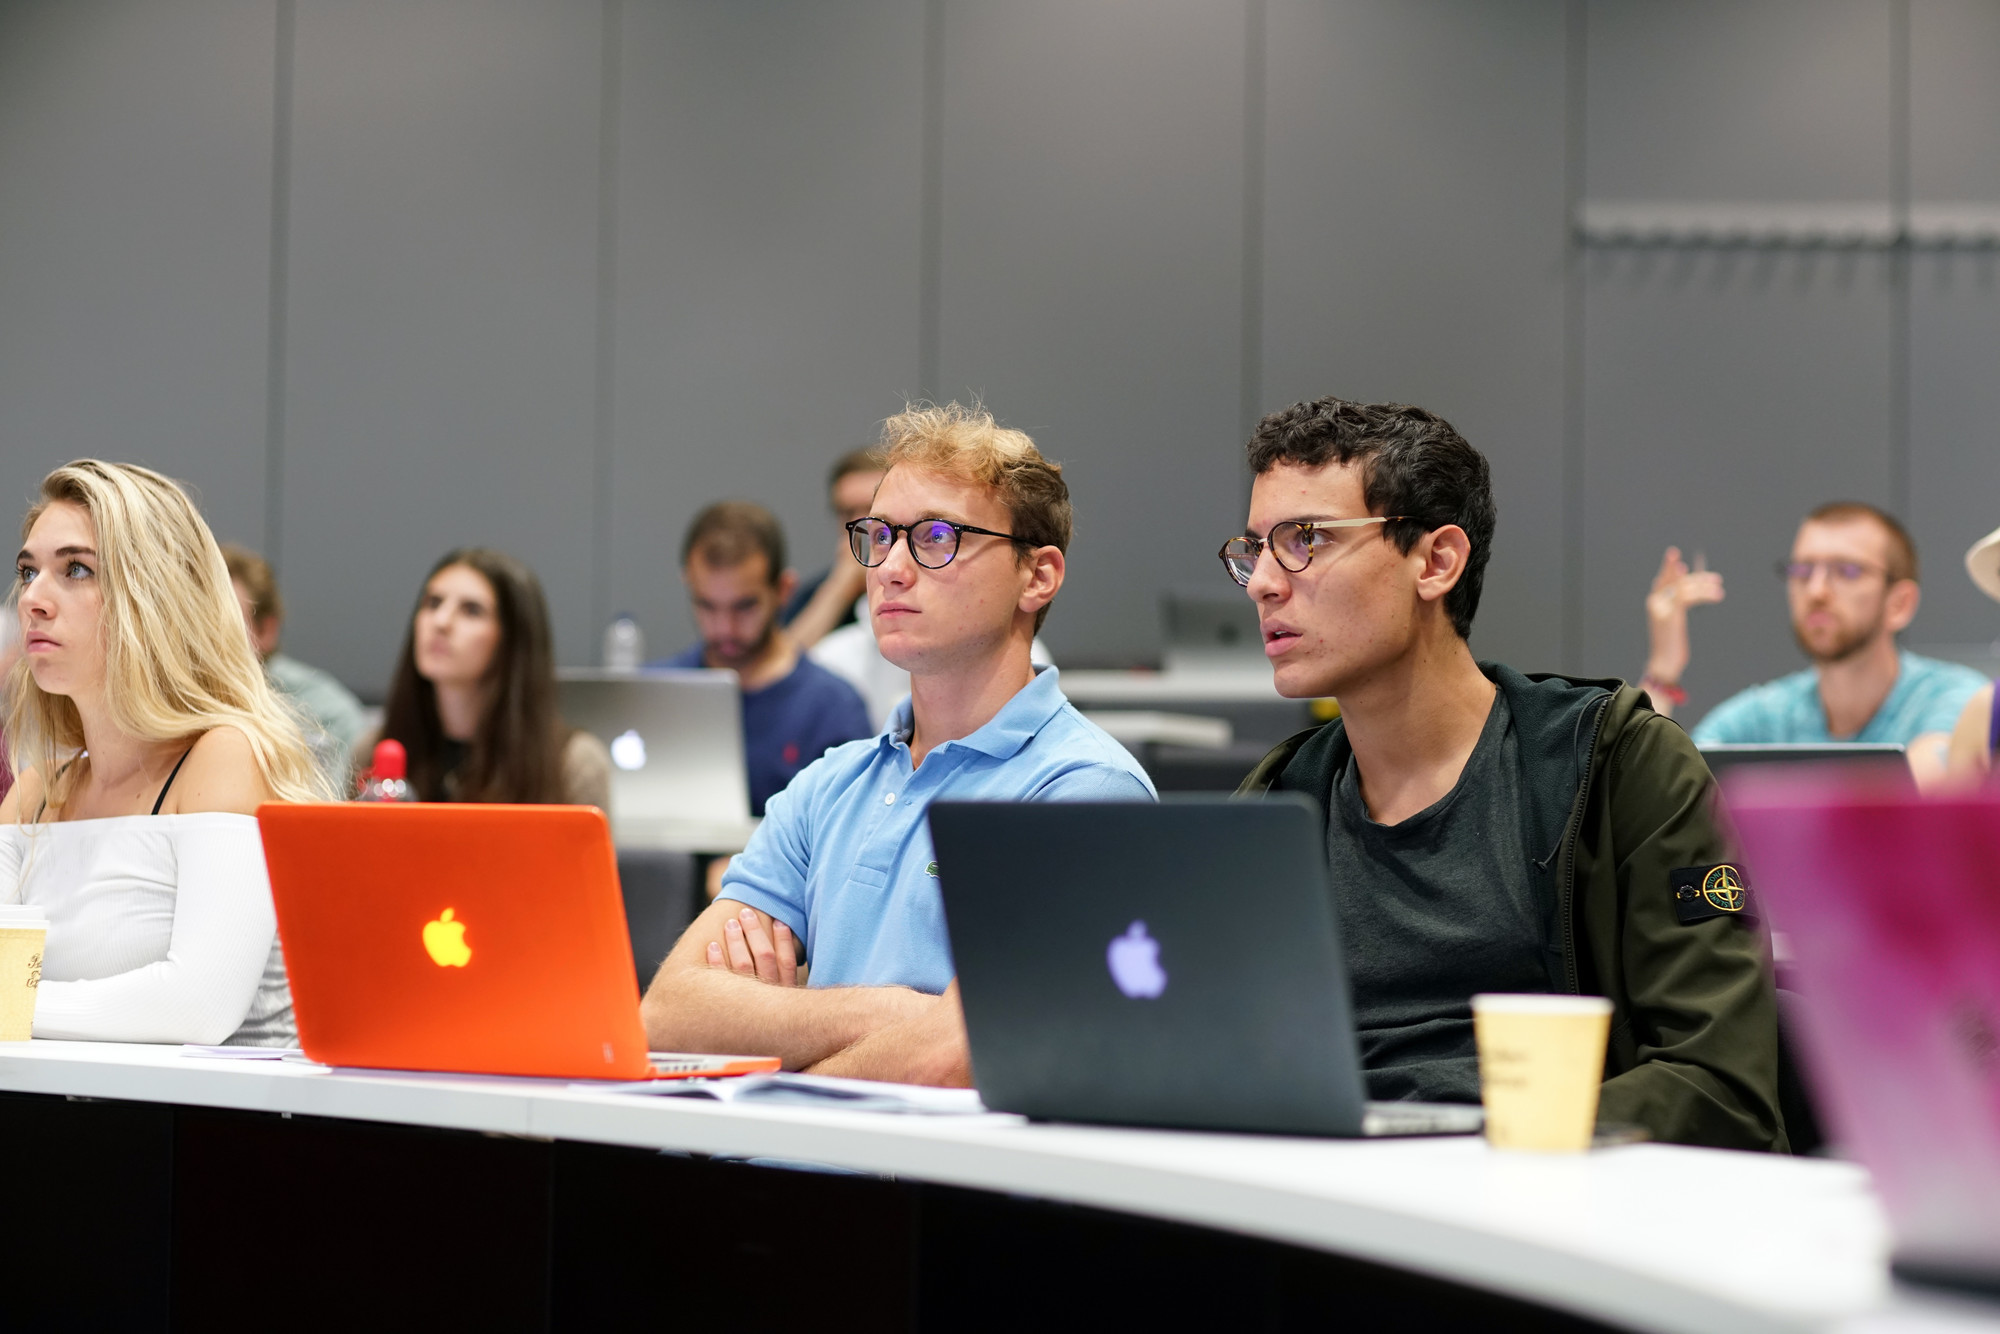
\includegraphics[width=\paperwidth]{abt_7295054328859831271Mjc0ODA1Ng.jpg}} % Slide background image

\begin{frame}[plain] % 'plain' suppresses the footer
\end{frame}
\endgroup

%------------------------------------------------

\begingroup
\setbeamertemplate{background}{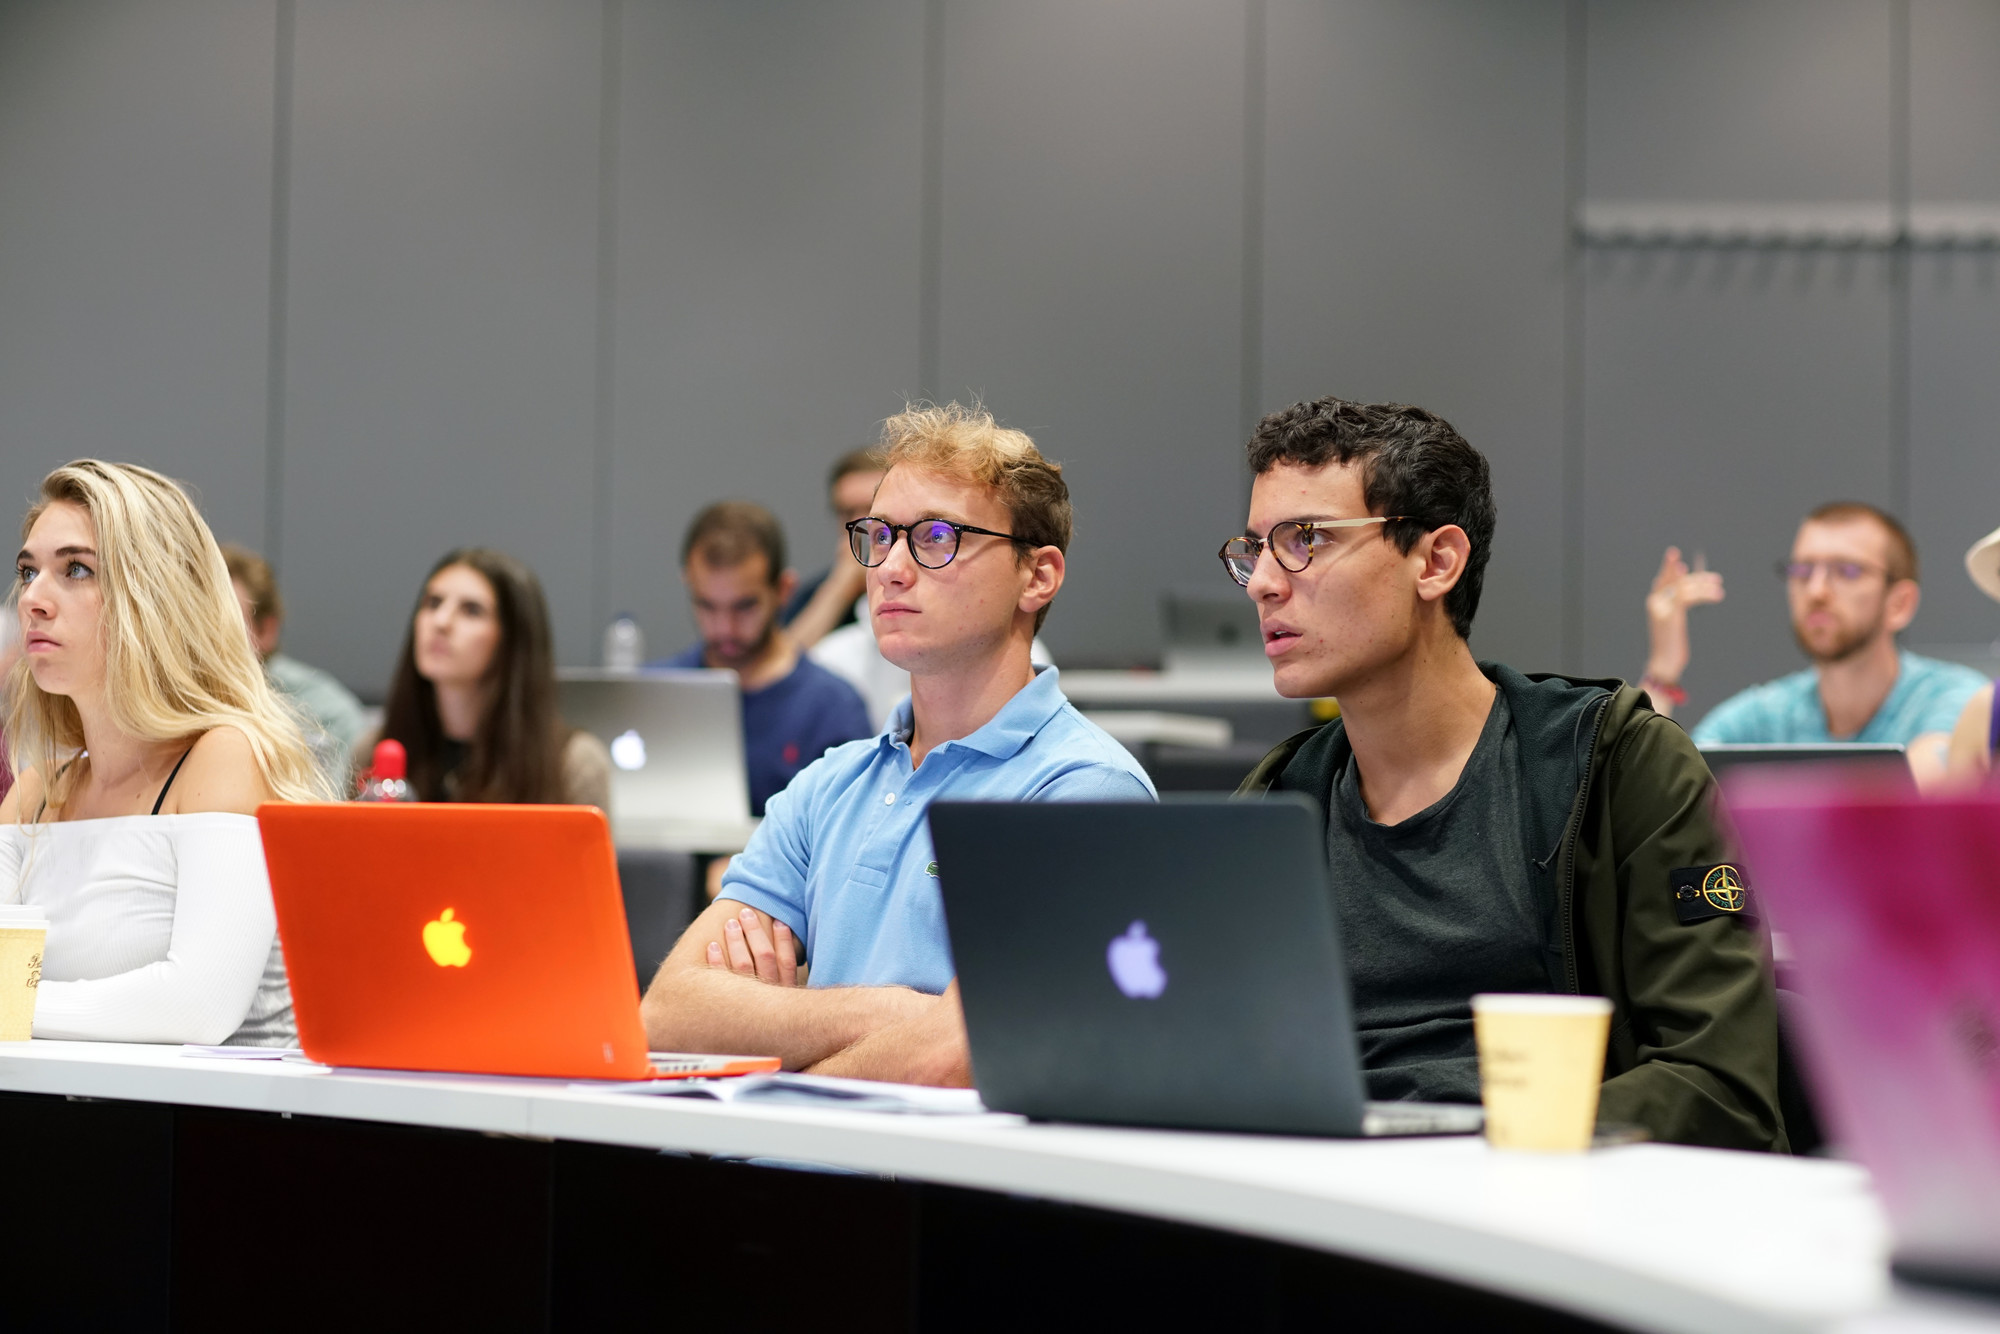
\includegraphics[width=\paperwidth]{abt_7295054328859831271Mjc0ODA1Ng.jpg}} % Slide background image
\setbeamercolor{normal text}{fg=white}\usebeamercolor[fg]{normal text} % Slide text color
\setbeamercolor{page number in head/foot}{fg=white} % Footer text color

\begin{frame}
    Text can be included on slides with image backgrounds too.
\end{frame}
\endgroup

%------------------------------------------------

\begin{frame}
    \frametitle{Slide Title}
    \framesubtitle{Tiled Images Example}

    \small % Reduce font size in this slide

    \begin{columns}[T] % [T] ensures correct vertical alignment
        \begin{column}{0.3\linewidth} % Left column
            \textbf{Section Title}\\
            Sed et mincipidem am fugia venihi aut utatem invellupis dolore voluptatiate veor mo dolendi squatur?

            Ab illate sitate explibus reiundusam, voluptur sim idebit, omnis dero quas adio quatur?
        \end{column}
        \begin{column}{0.68\linewidth} % Right column
            \vspace{-3.5\baselineskip} % Pull images up

            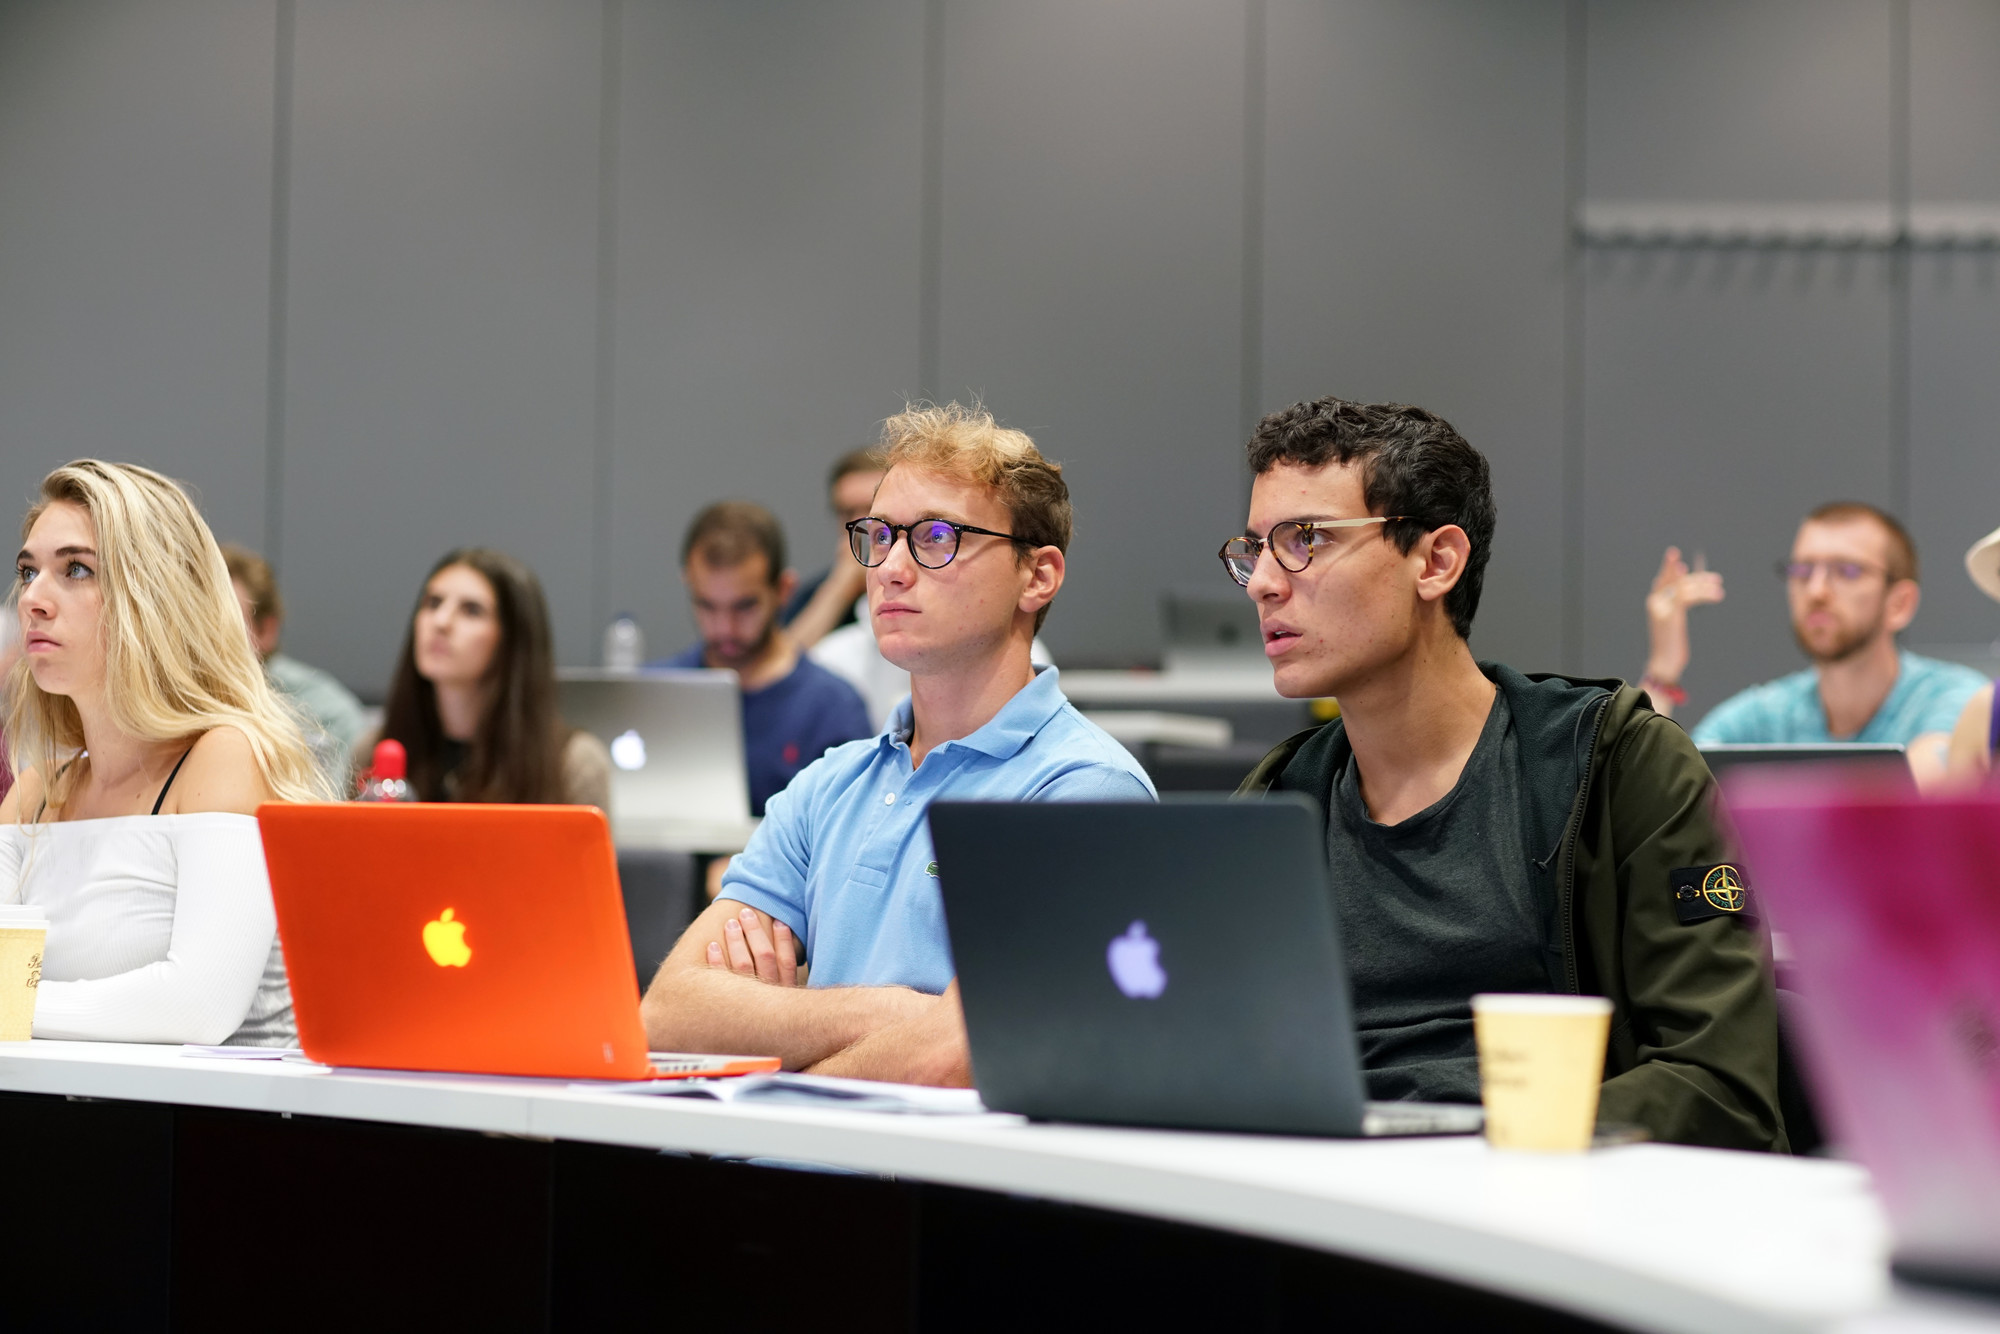
\includegraphics[width=0.32\linewidth]{abt_7295054328859831271Mjc0ODA1Ng.jpg}\hfill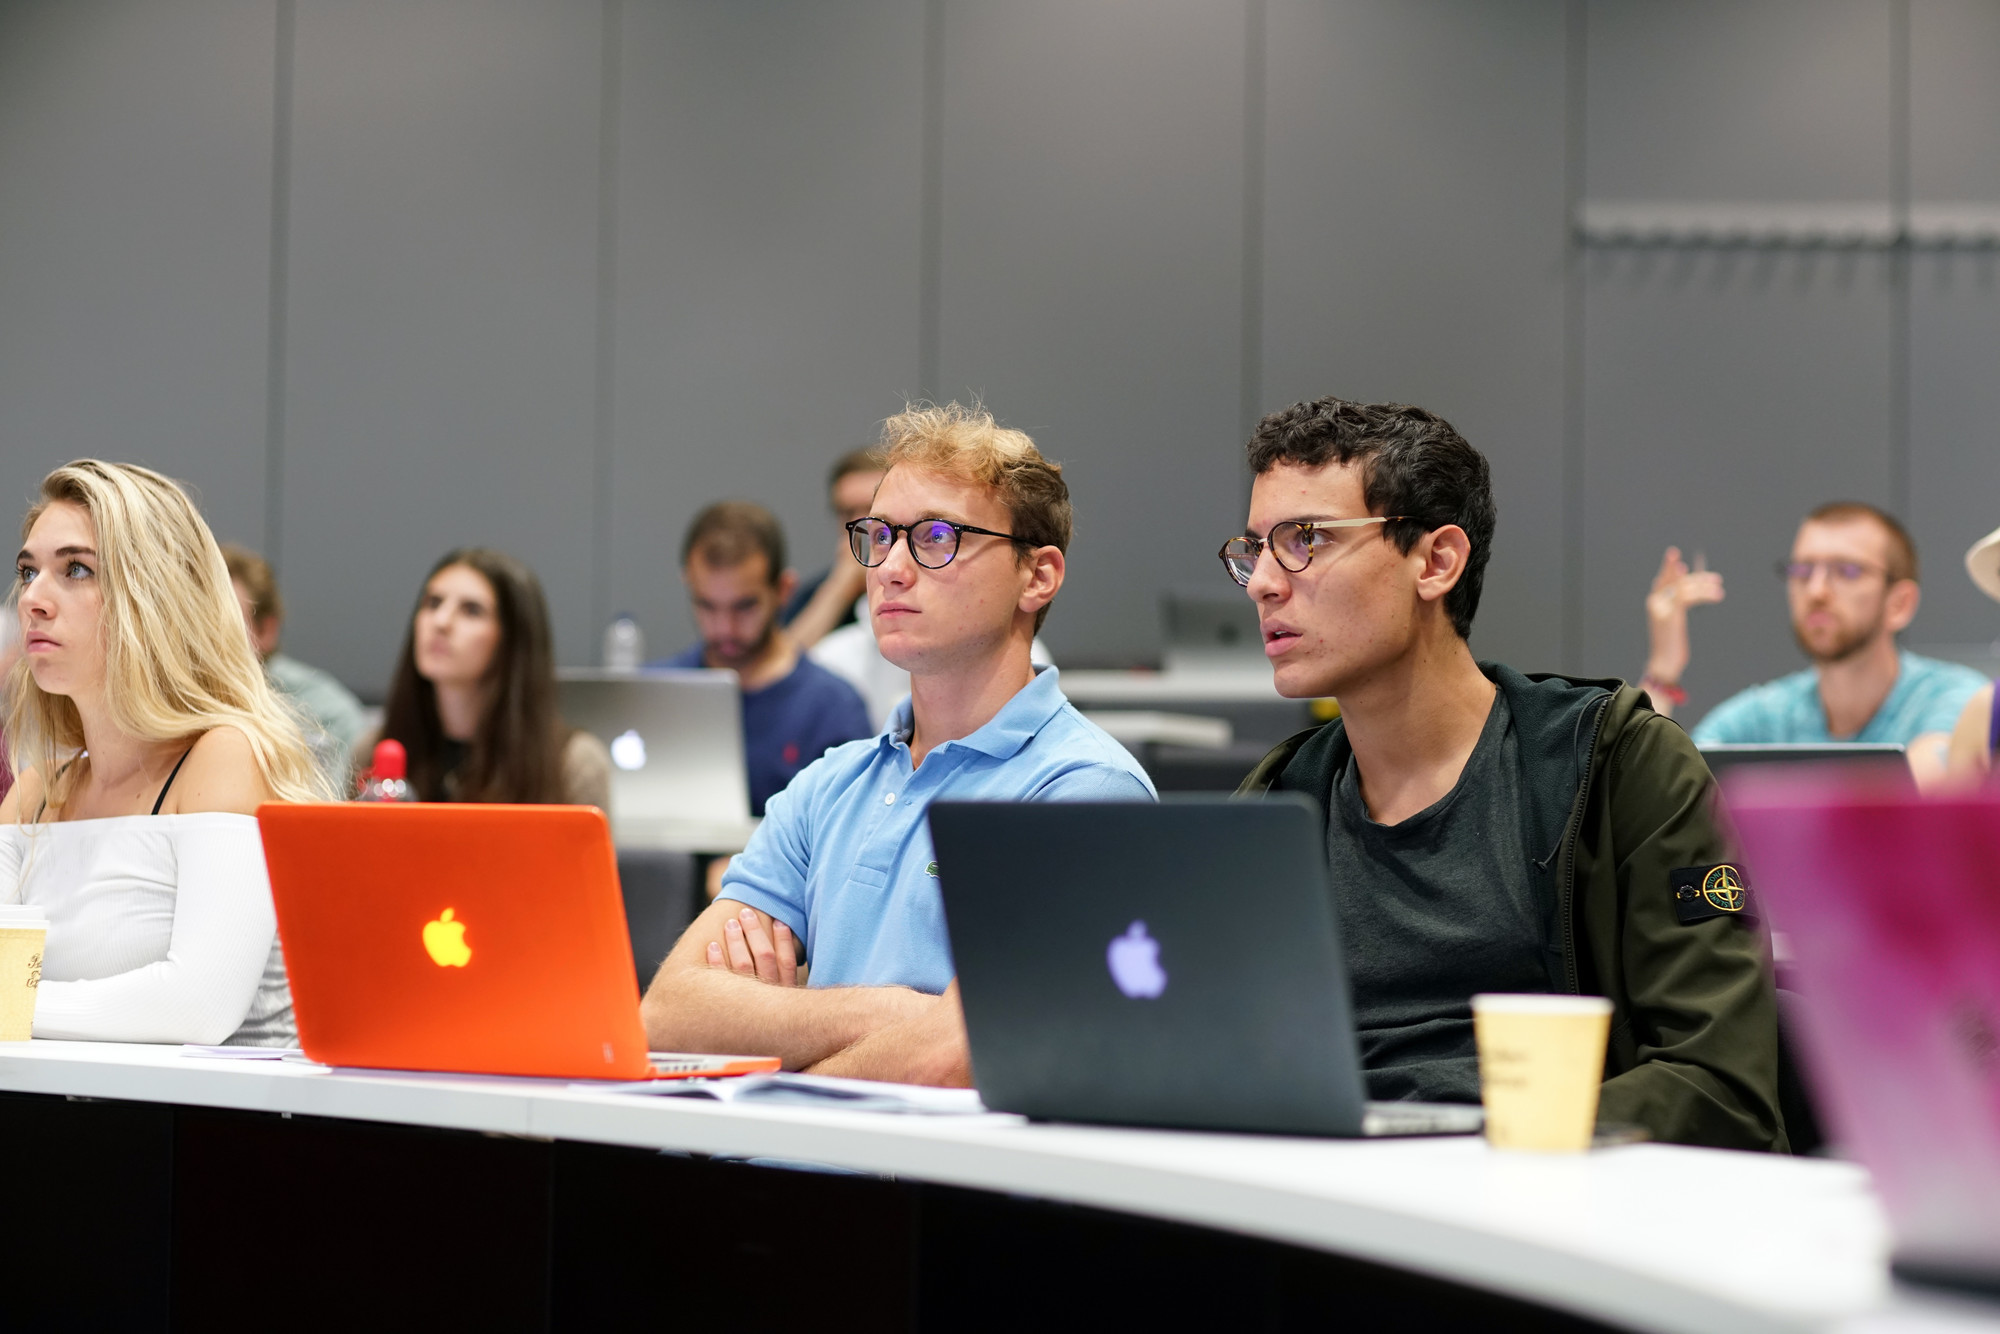
\includegraphics[width=0.32\linewidth]{abt_7295054328859831271Mjc0ODA1Ng.jpg}\hfill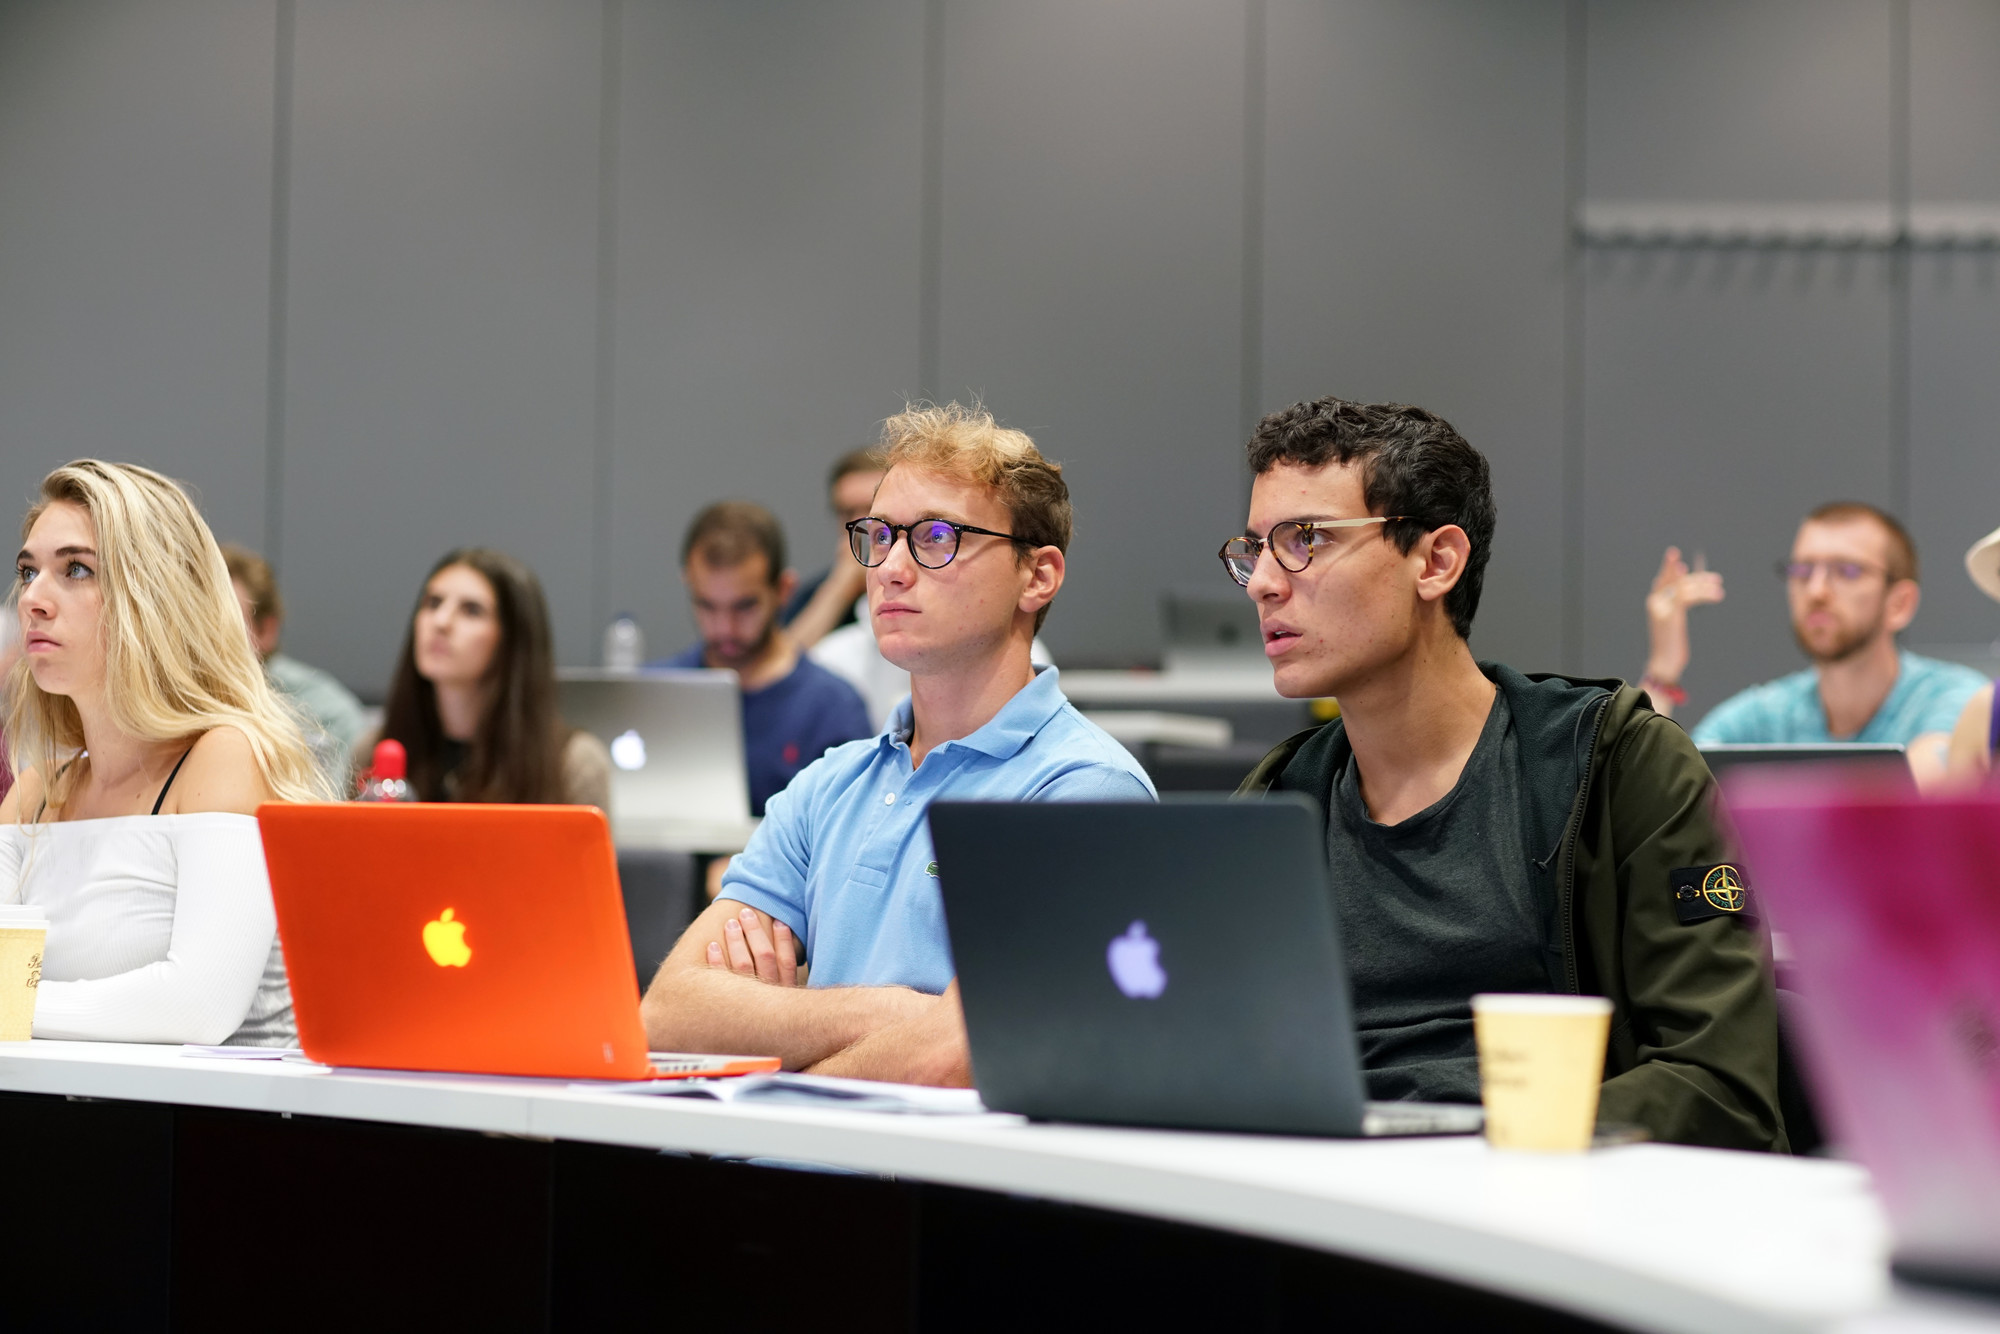
\includegraphics[width=0.32\linewidth]{abt_7295054328859831271Mjc0ODA1Ng.jpg}\\[6pt]
            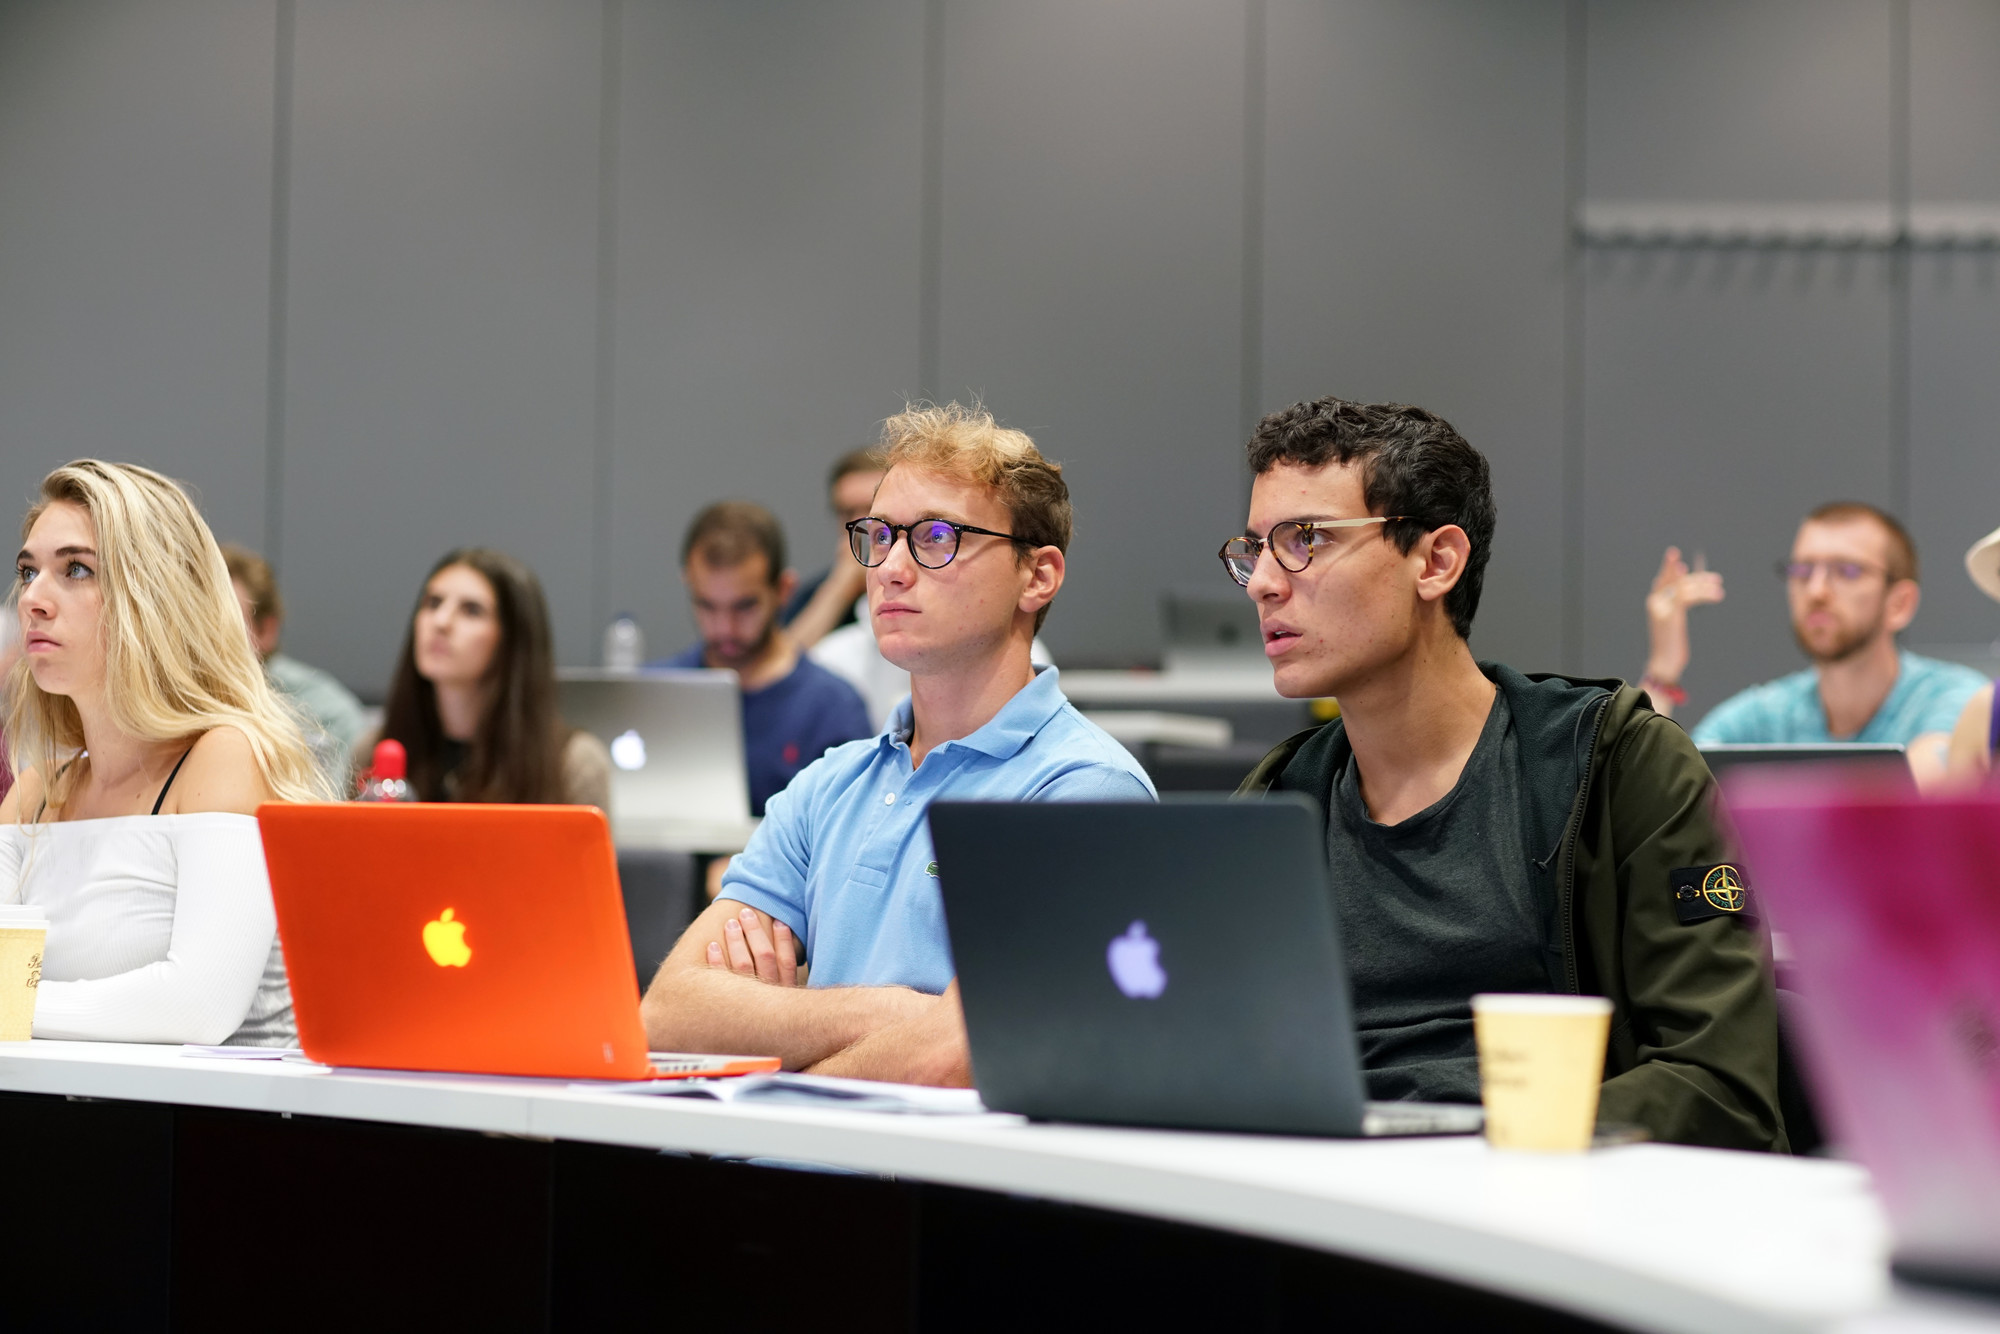
\includegraphics[width=0.32\linewidth]{abt_7295054328859831271Mjc0ODA1Ng.jpg}\hfill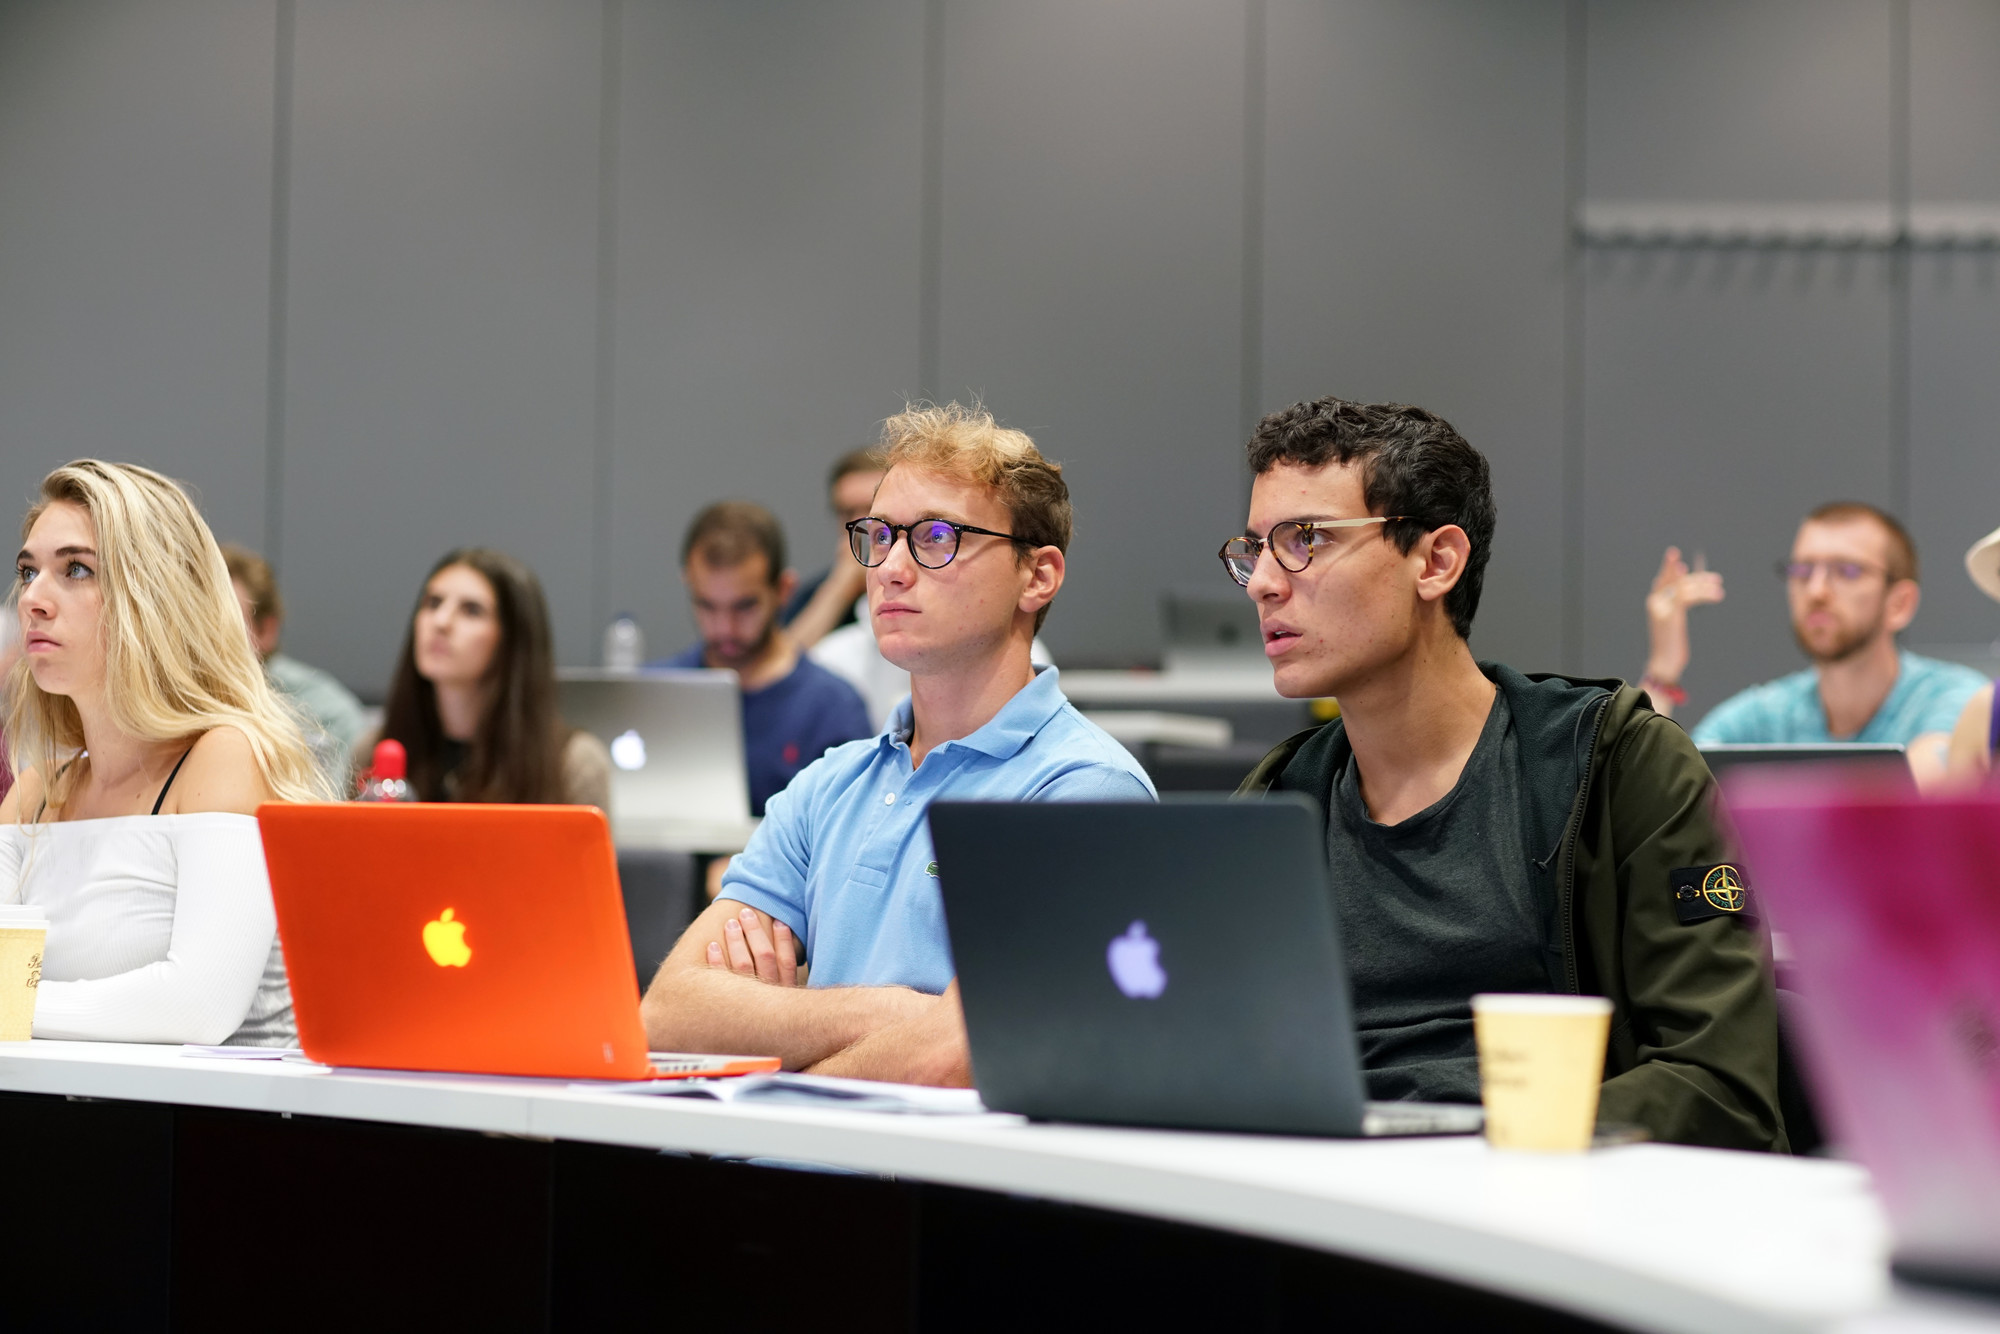
\includegraphics[width=0.32\linewidth]{abt_7295054328859831271Mjc0ODA1Ng.jpg}\hfill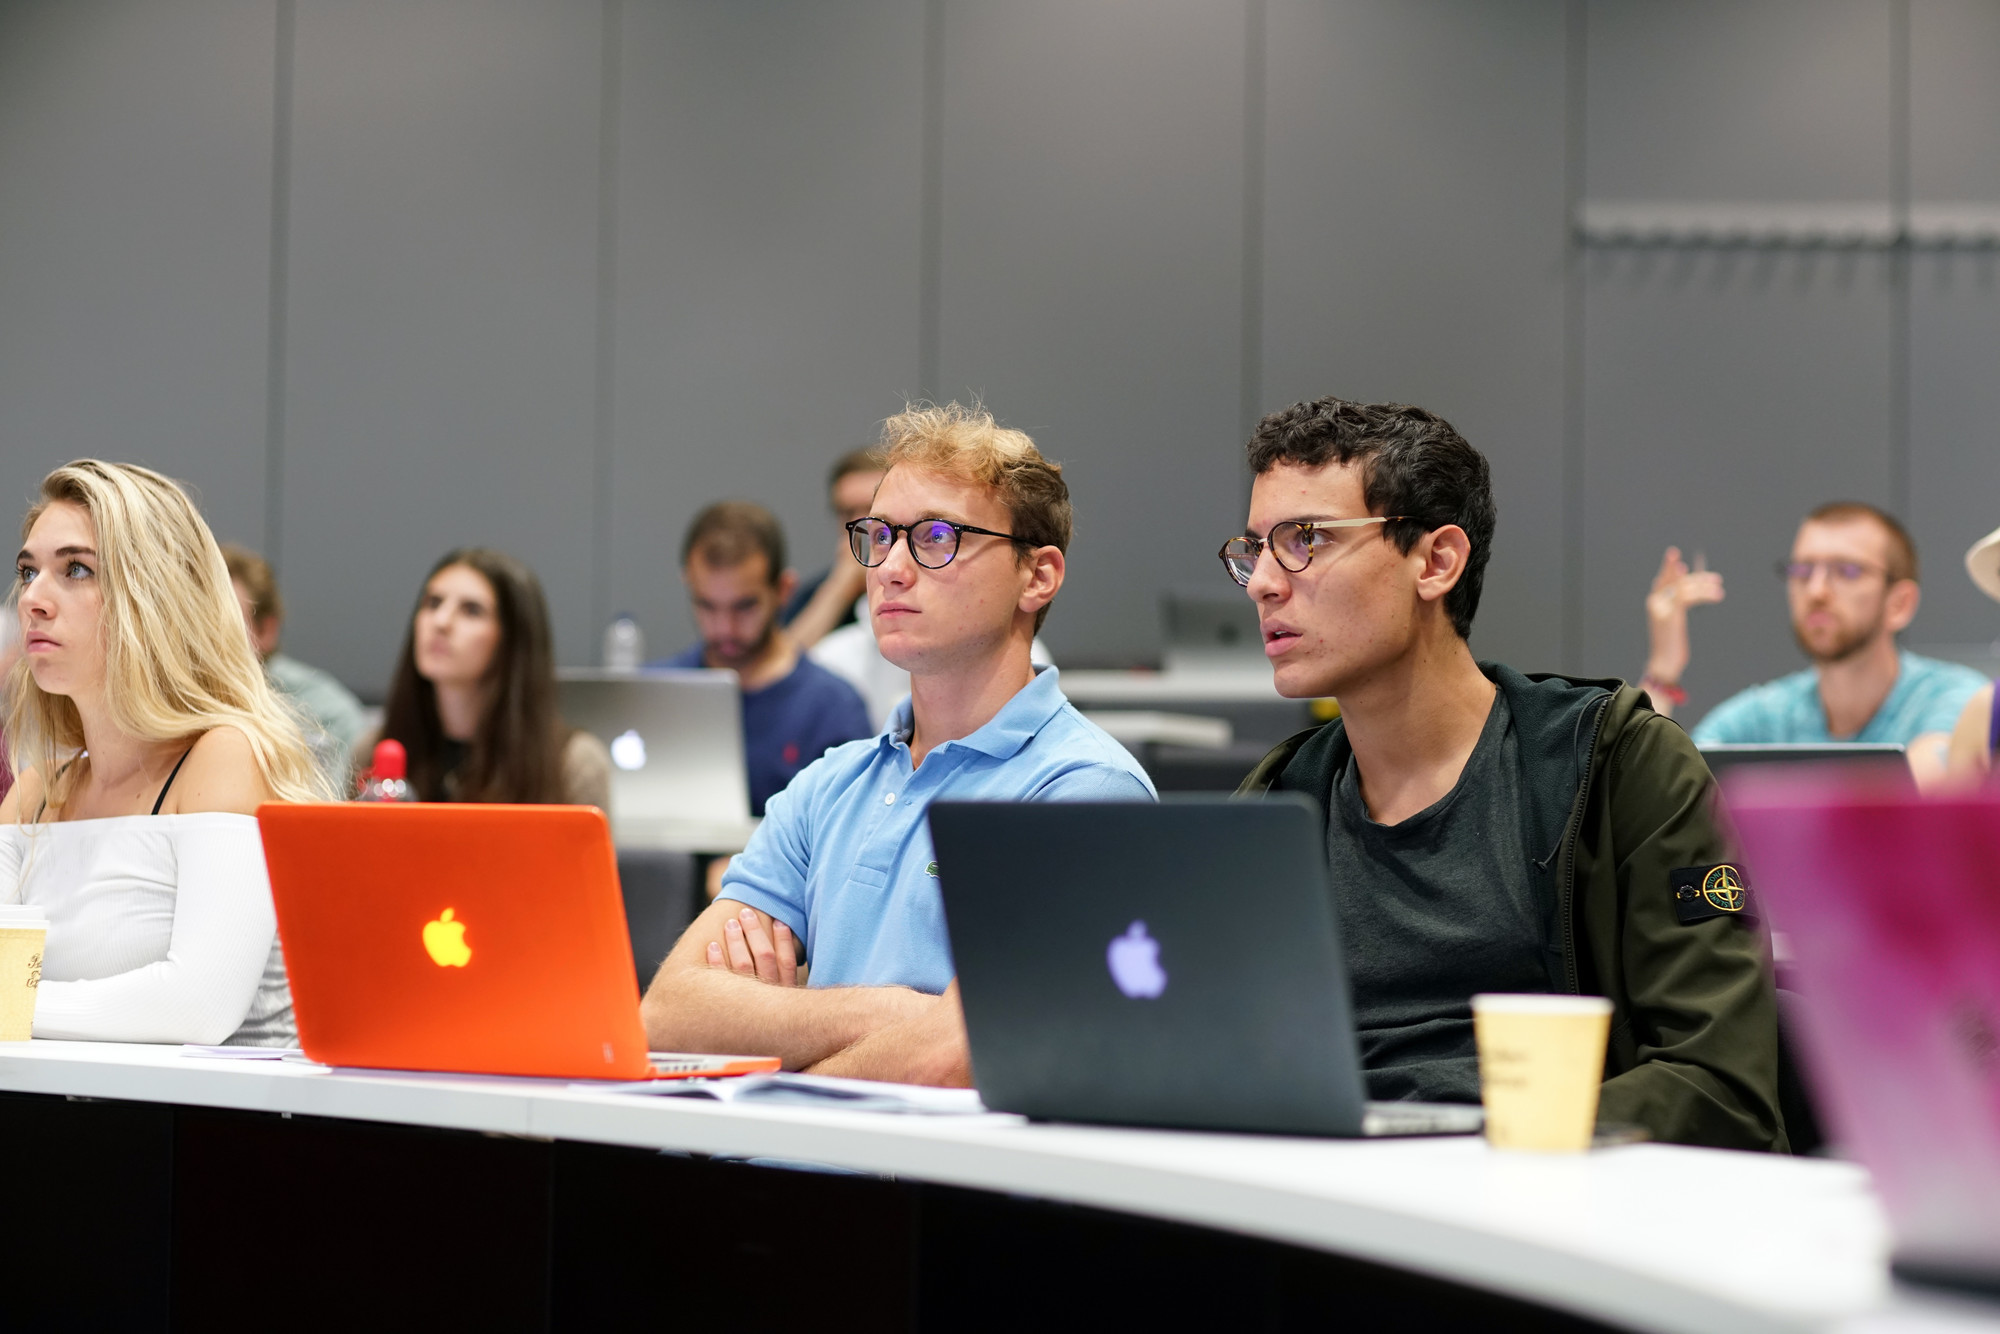
\includegraphics[width=0.32\linewidth]{abt_7295054328859831271Mjc0ODA1Ng.jpg}\\[6pt]
            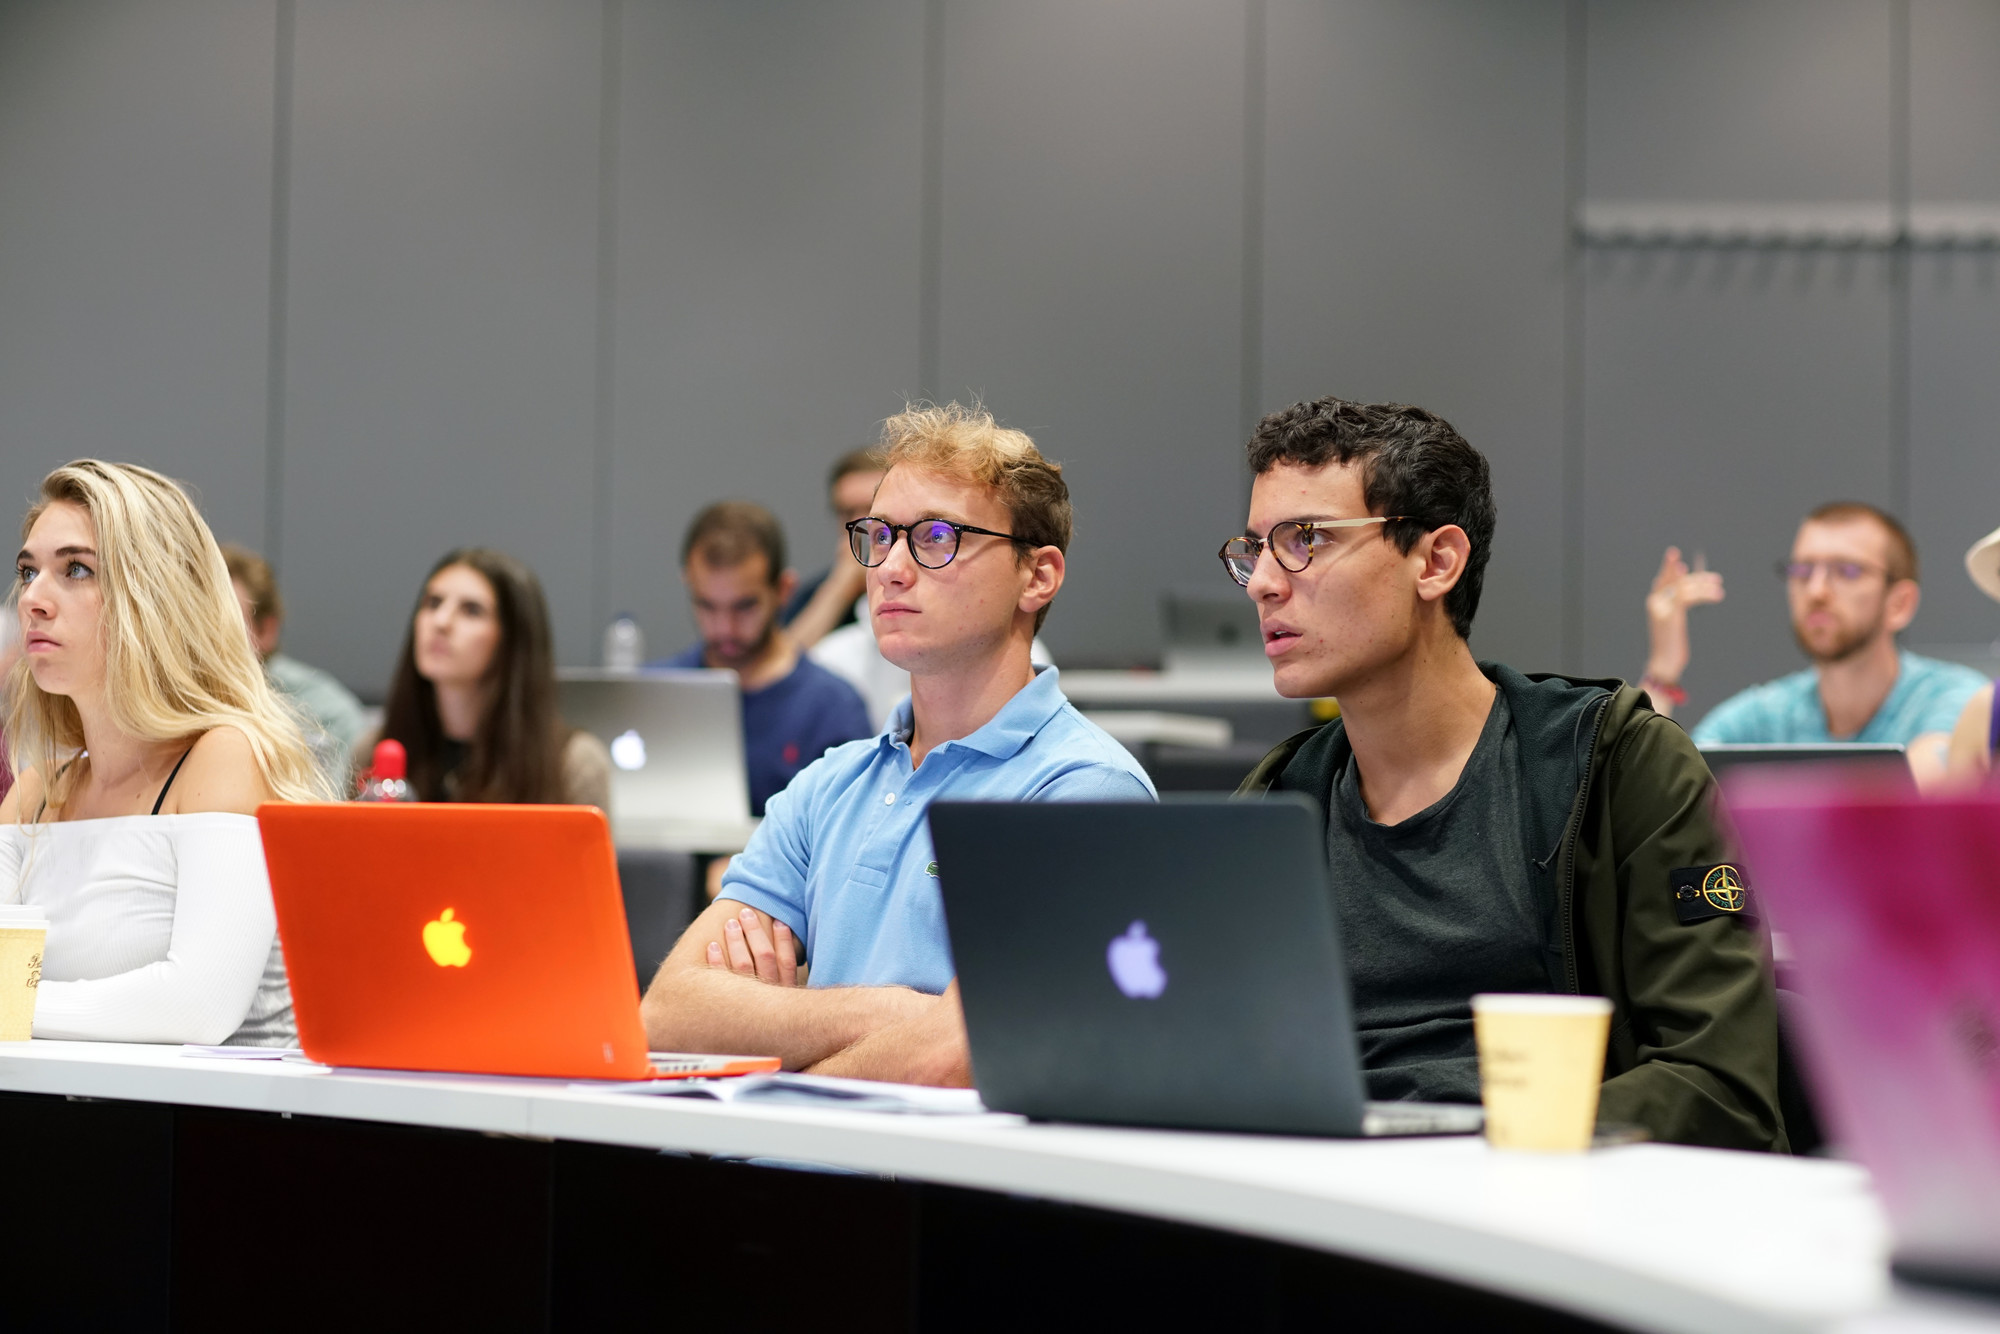
\includegraphics[width=0.32\linewidth]{abt_7295054328859831271Mjc0ODA1Ng.jpg}\hfill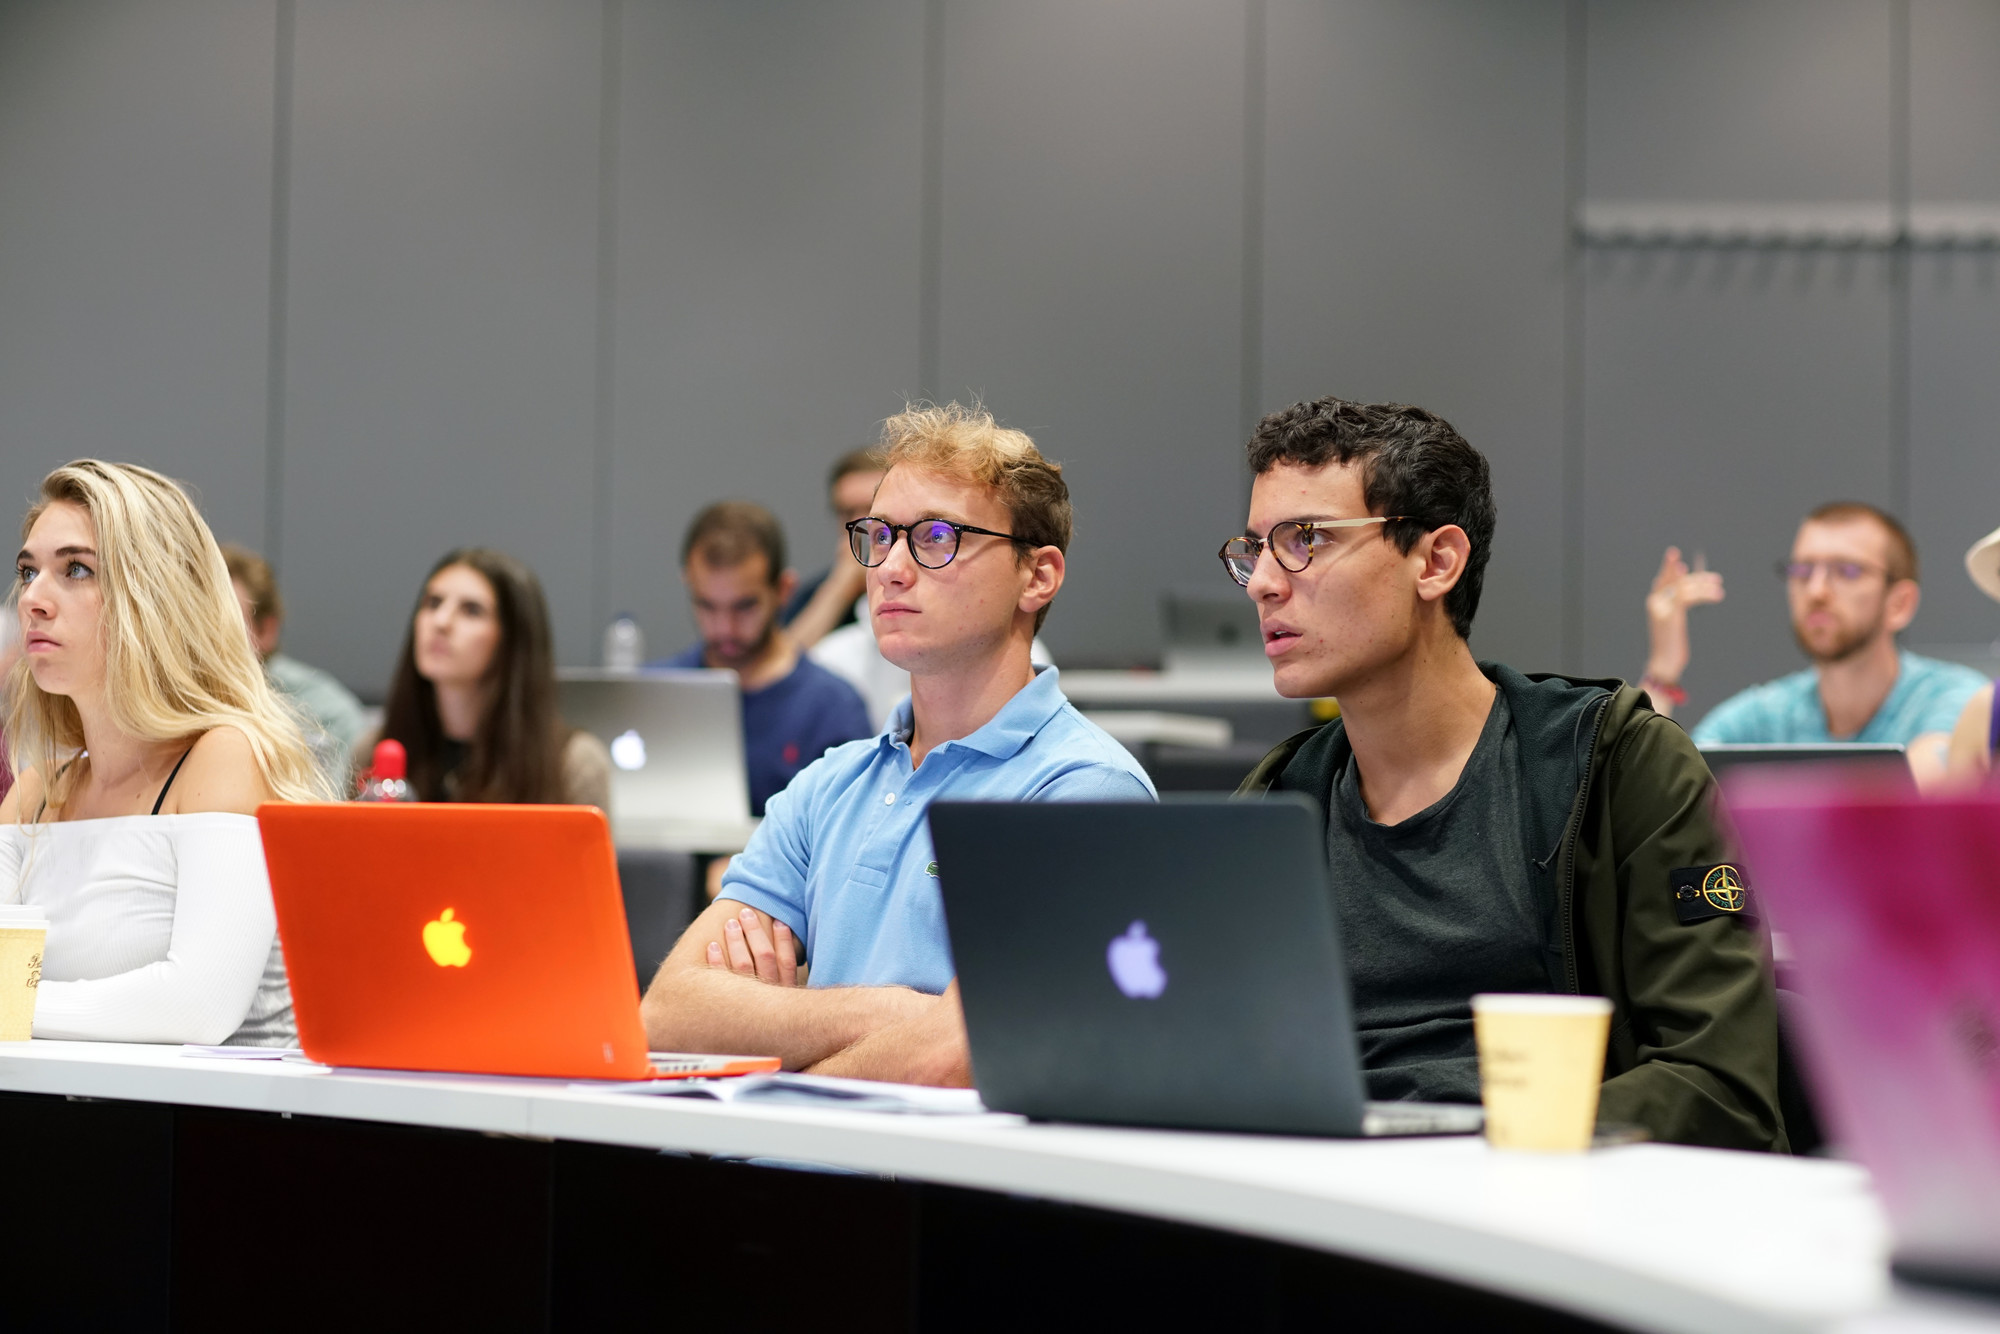
\includegraphics[width=0.32\linewidth]{abt_7295054328859831271Mjc0ODA1Ng.jpg}\hfill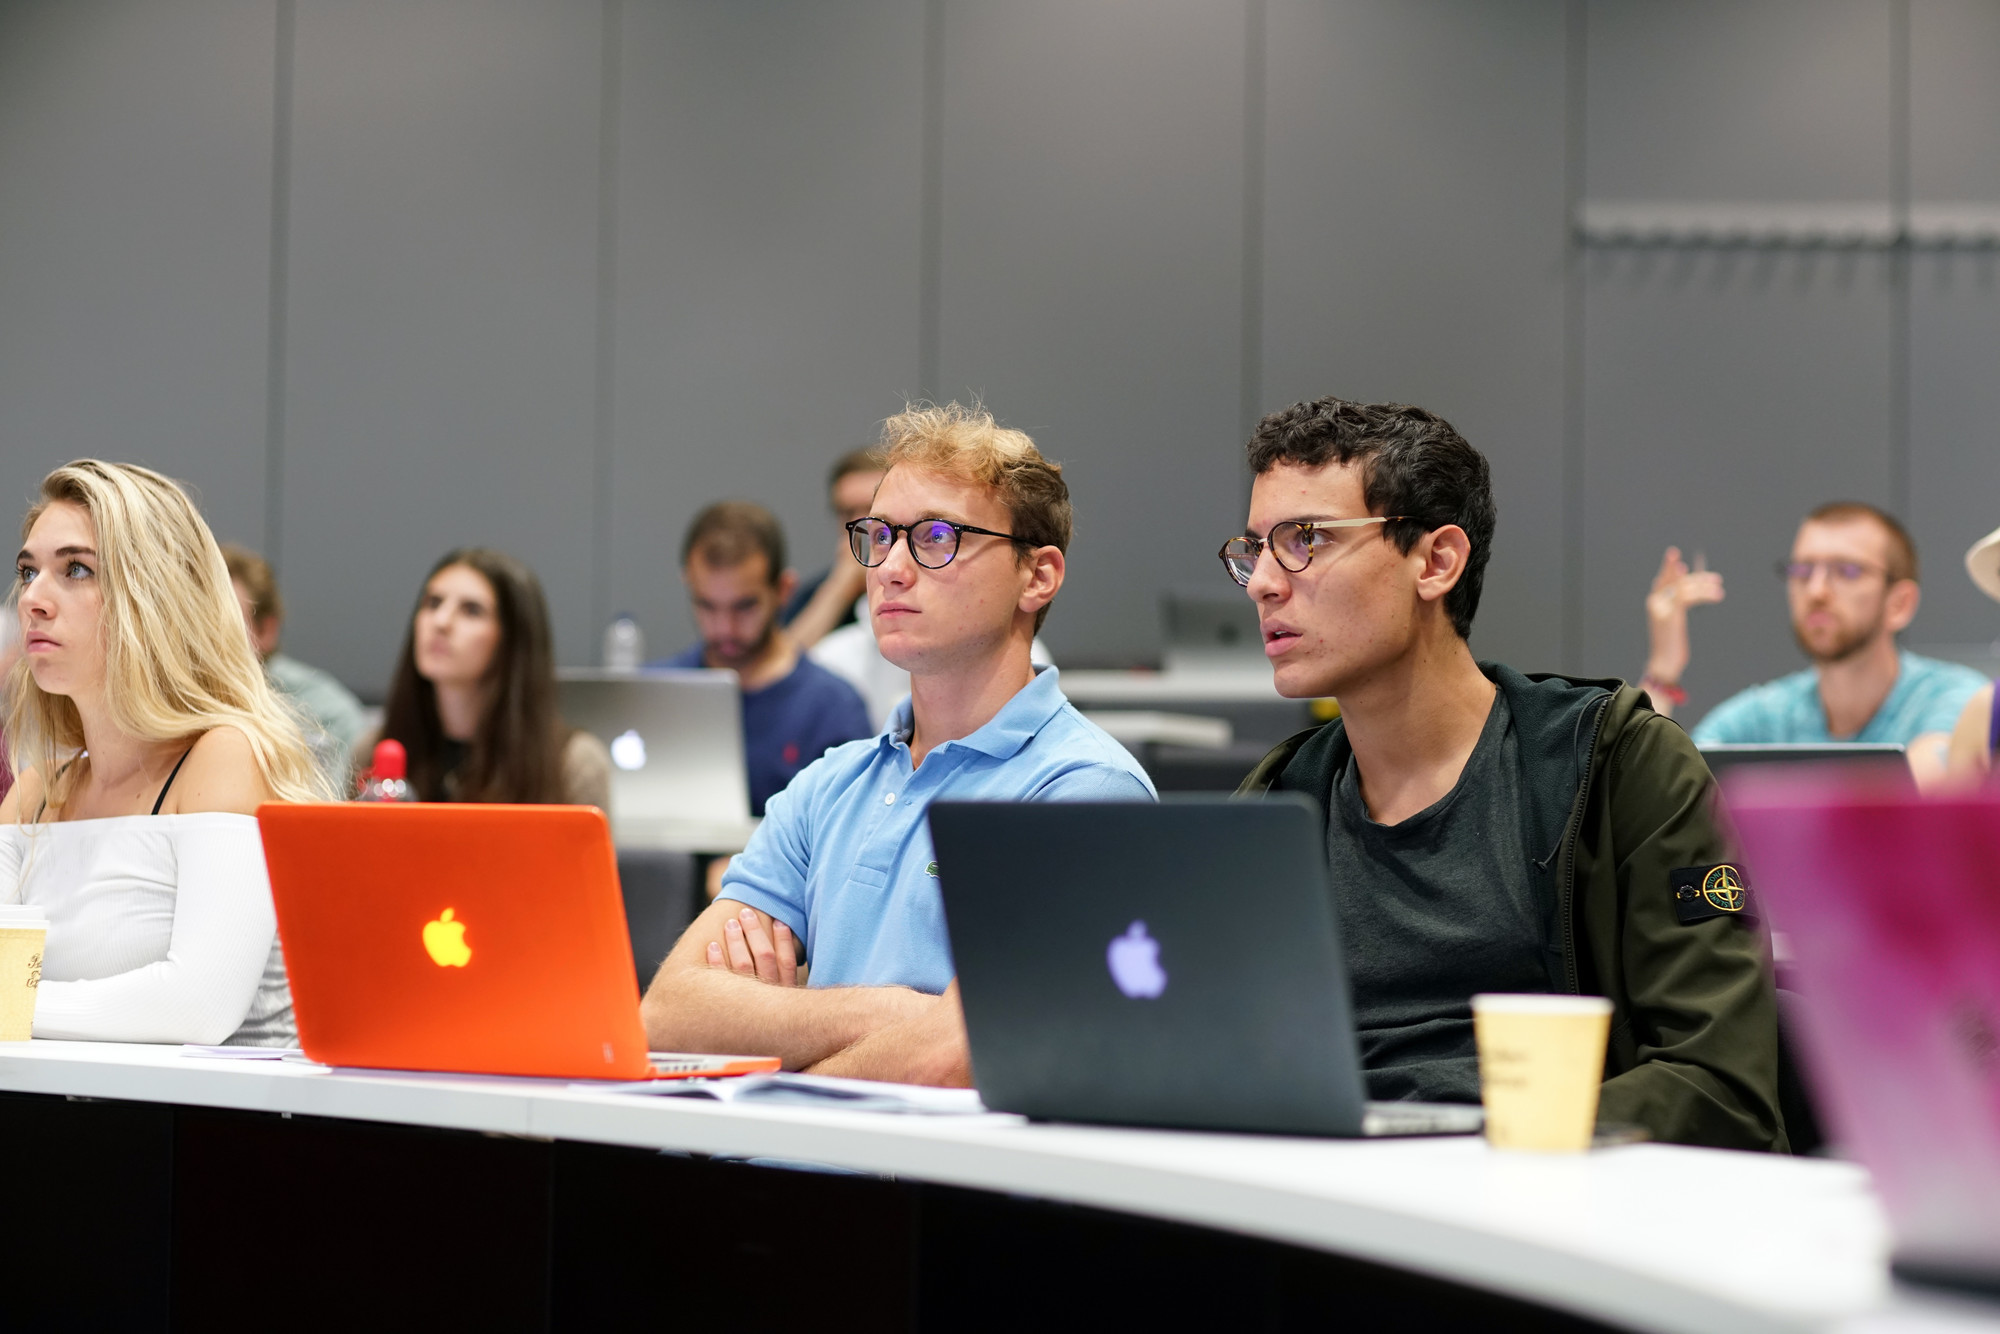
\includegraphics[width=0.32\linewidth]{abt_7295054328859831271Mjc0ODA1Ng.jpg}\par
        \end{column}
    \end{columns}
\end{frame}

%------------------------------------------------

\begin{frame}
    \frametitle{Slide Title}
    \framesubtitle{Tiled Images Example}

    \small % Reduce font size in this slide

    \begin{columns}[T] % [T] ensures correct vertical alignment
        \begin{column}{0.3\linewidth} % Left column
            \textbf{Section Title}\\
            Sed et mincipidem am fugia venihi aut utatem invellupis dolore voluptatiate veor mo dolendi squatur?

            Ab illate sitate explibus reiundusam, voluptur sim idebit, omnis dero quas adio quatur?
        \end{column}
        \begin{column}{0.68\linewidth} % Right column
            \vspace{-3.5\baselineskip} % Pull images up

            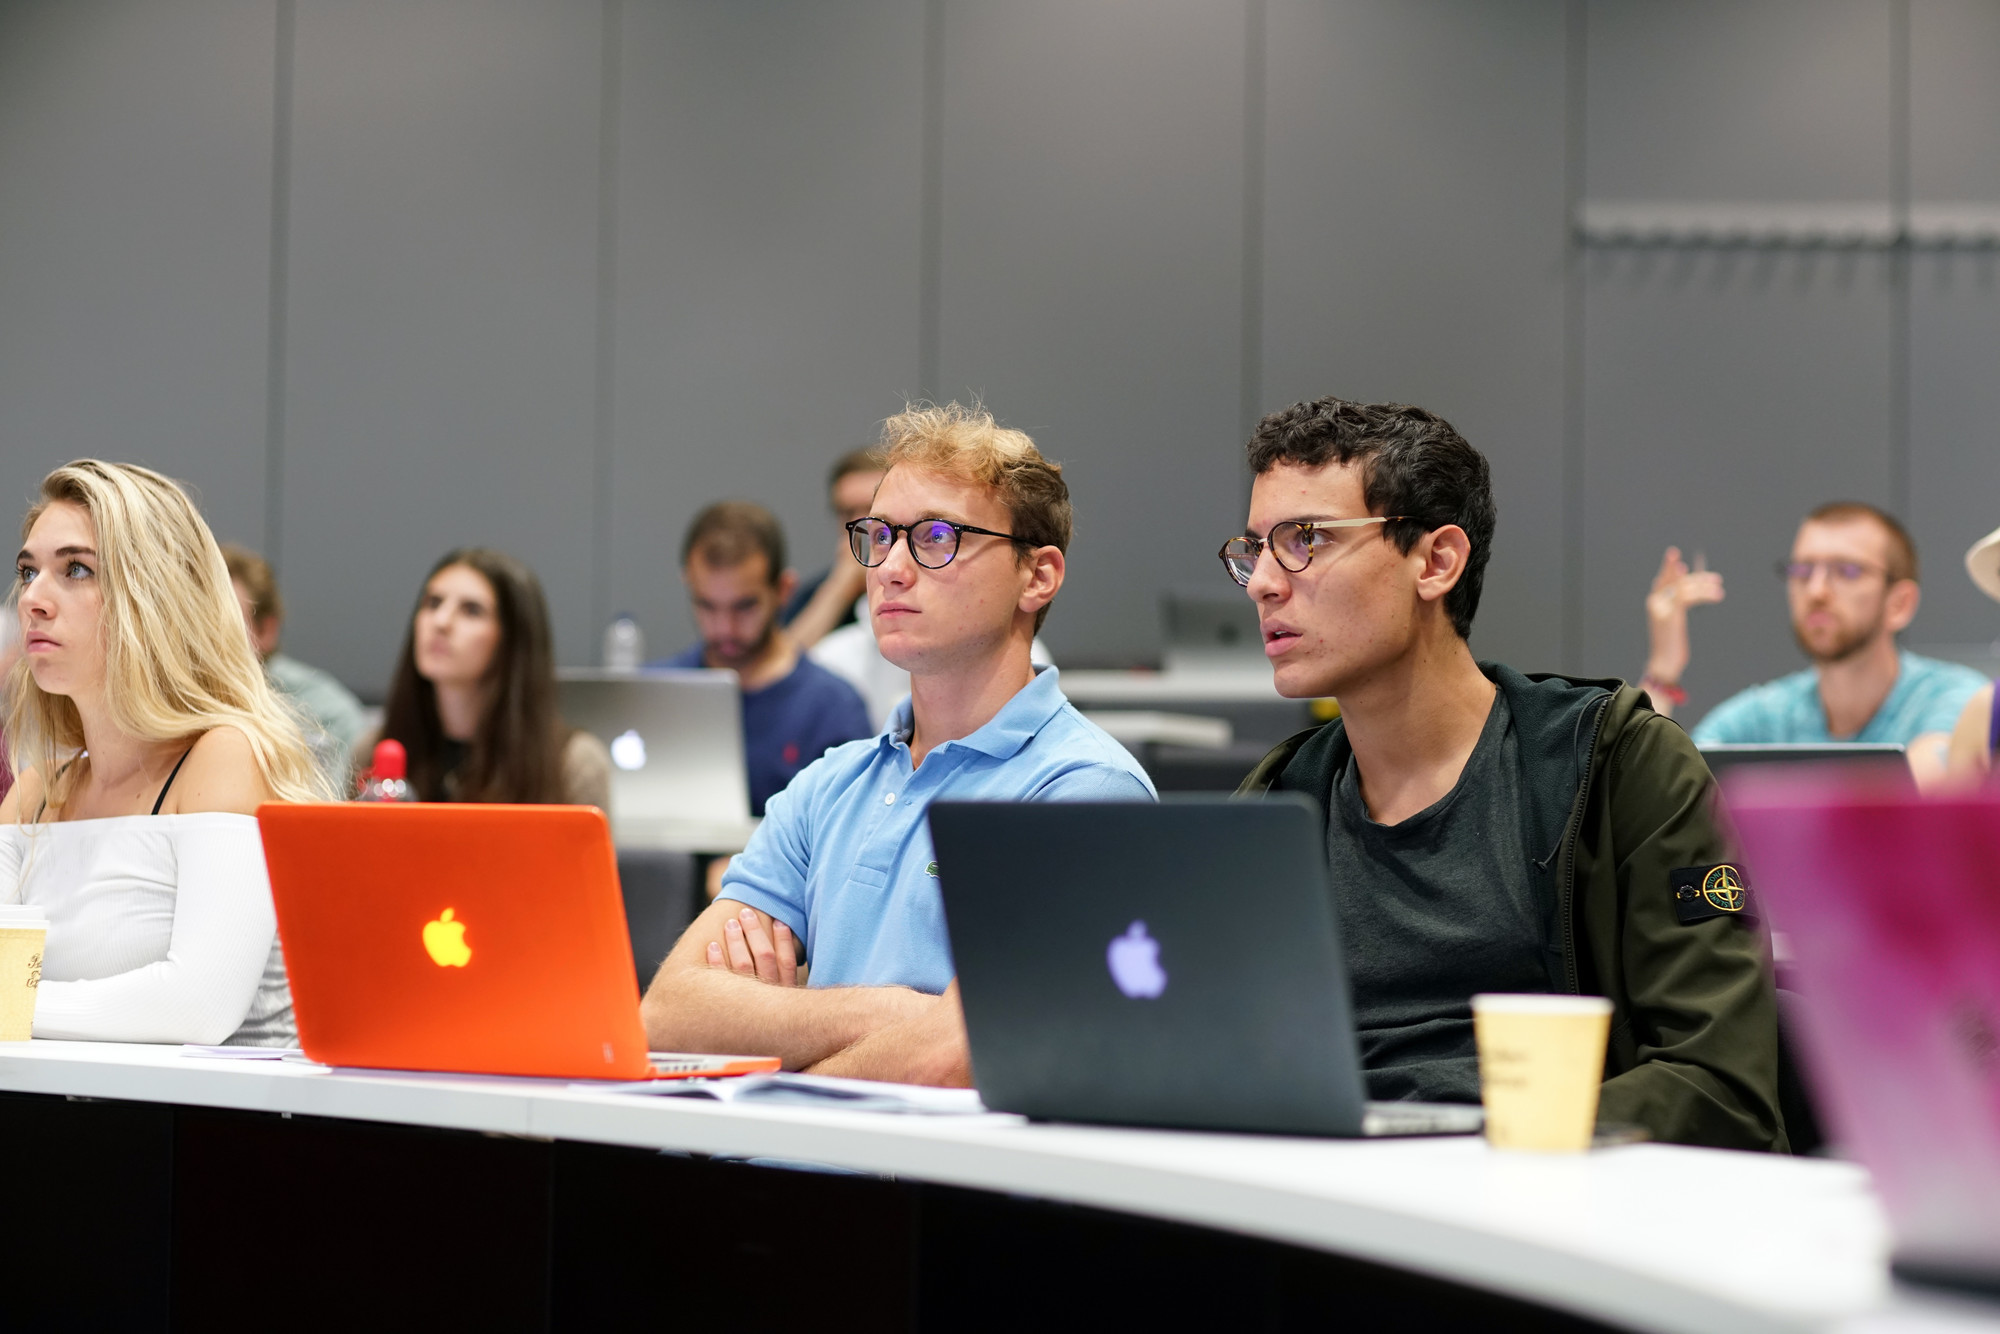
\includegraphics[width=0.495\linewidth]{abt_7295054328859831271Mjc0ODA1Ng.jpg}\hfill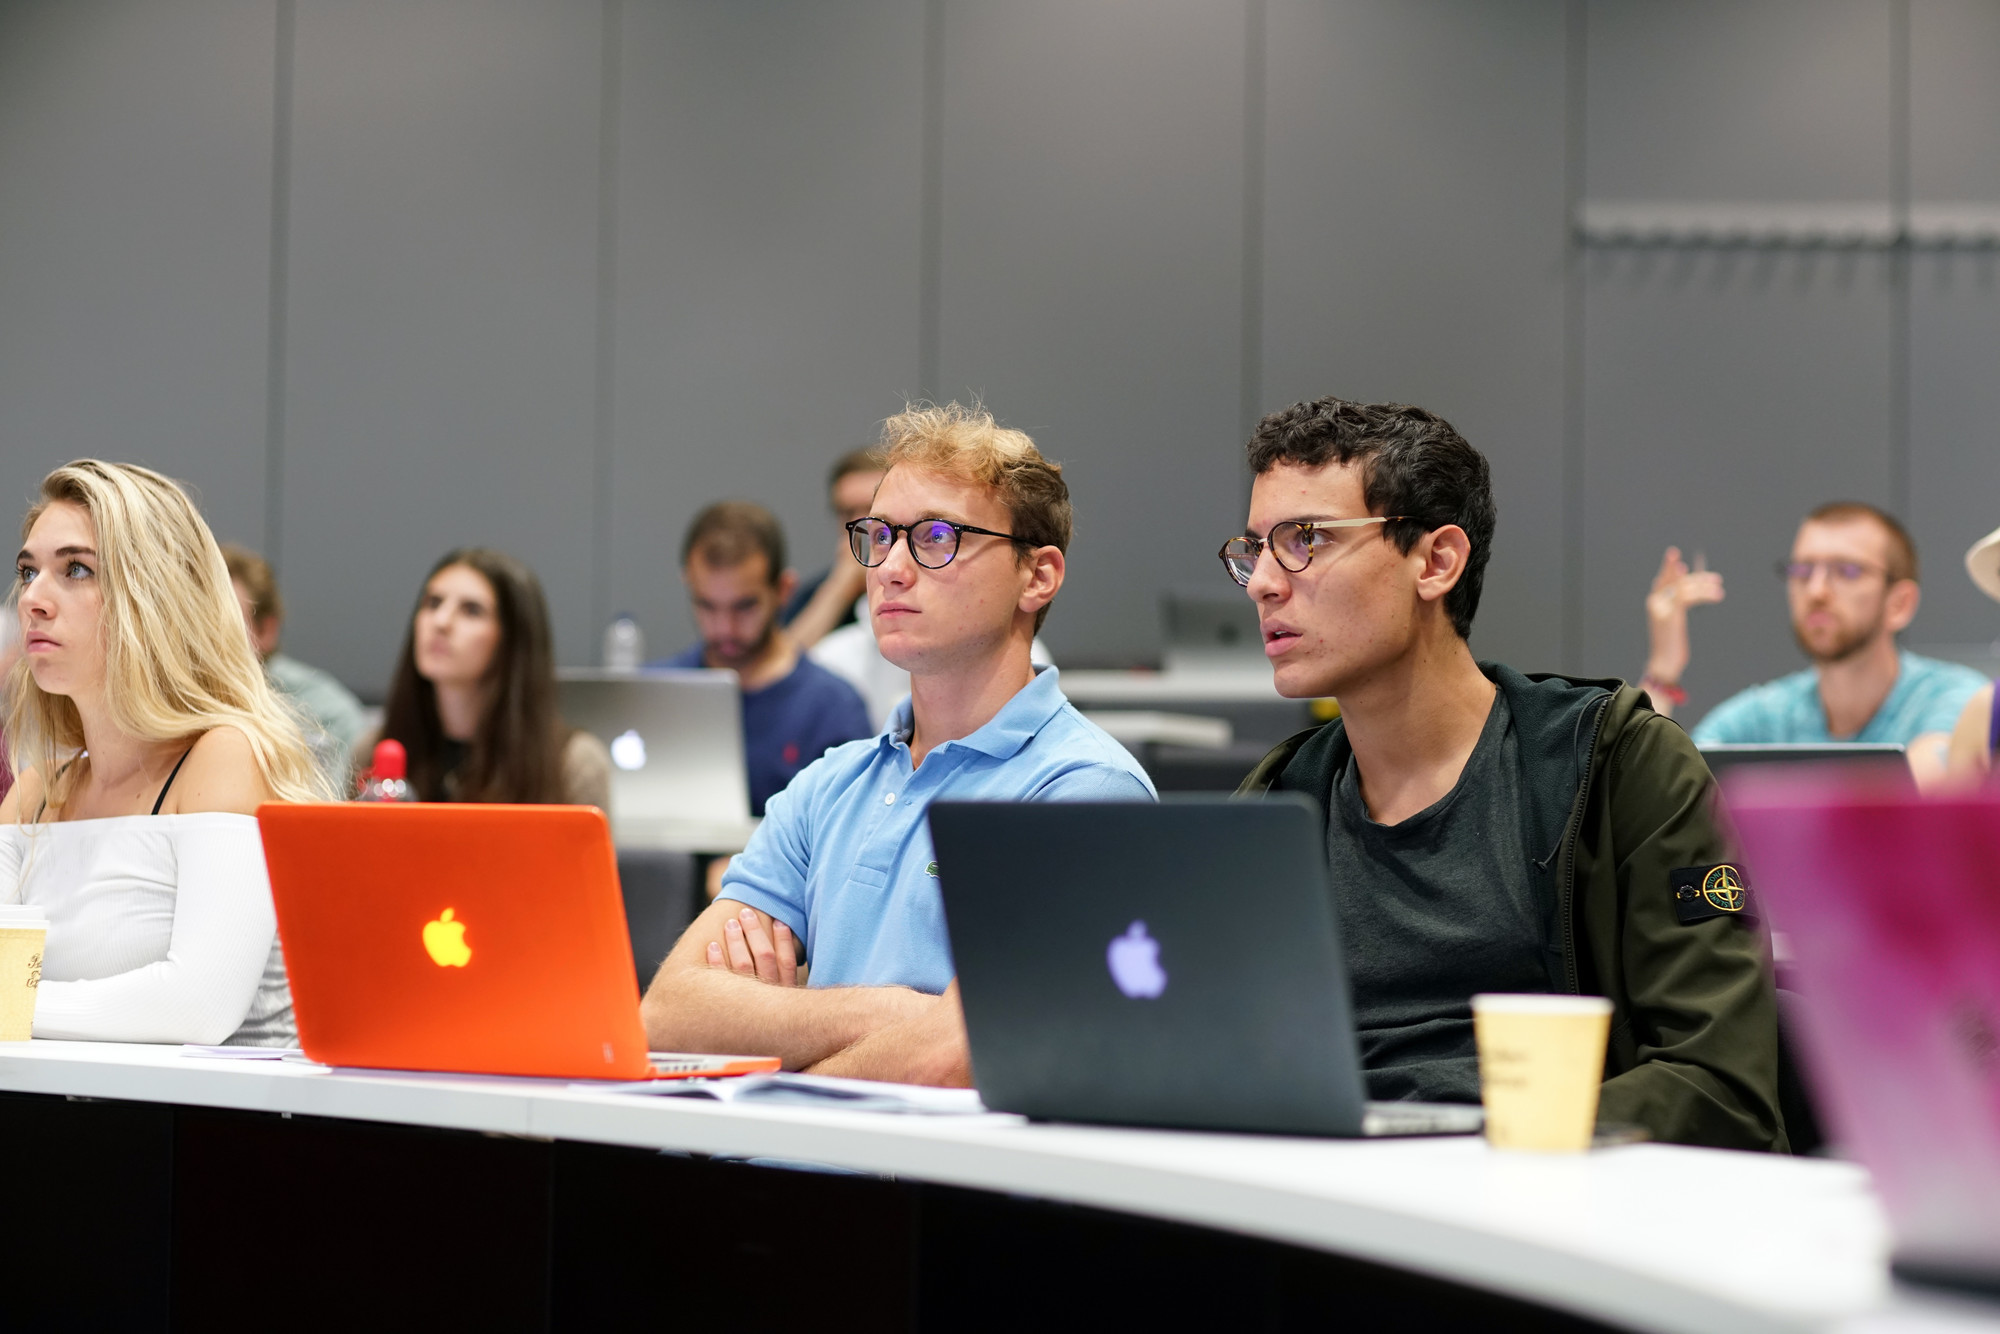
\includegraphics[width=0.495\linewidth]{abt_7295054328859831271Mjc0ODA1Ng.jpg}\\[4pt]
            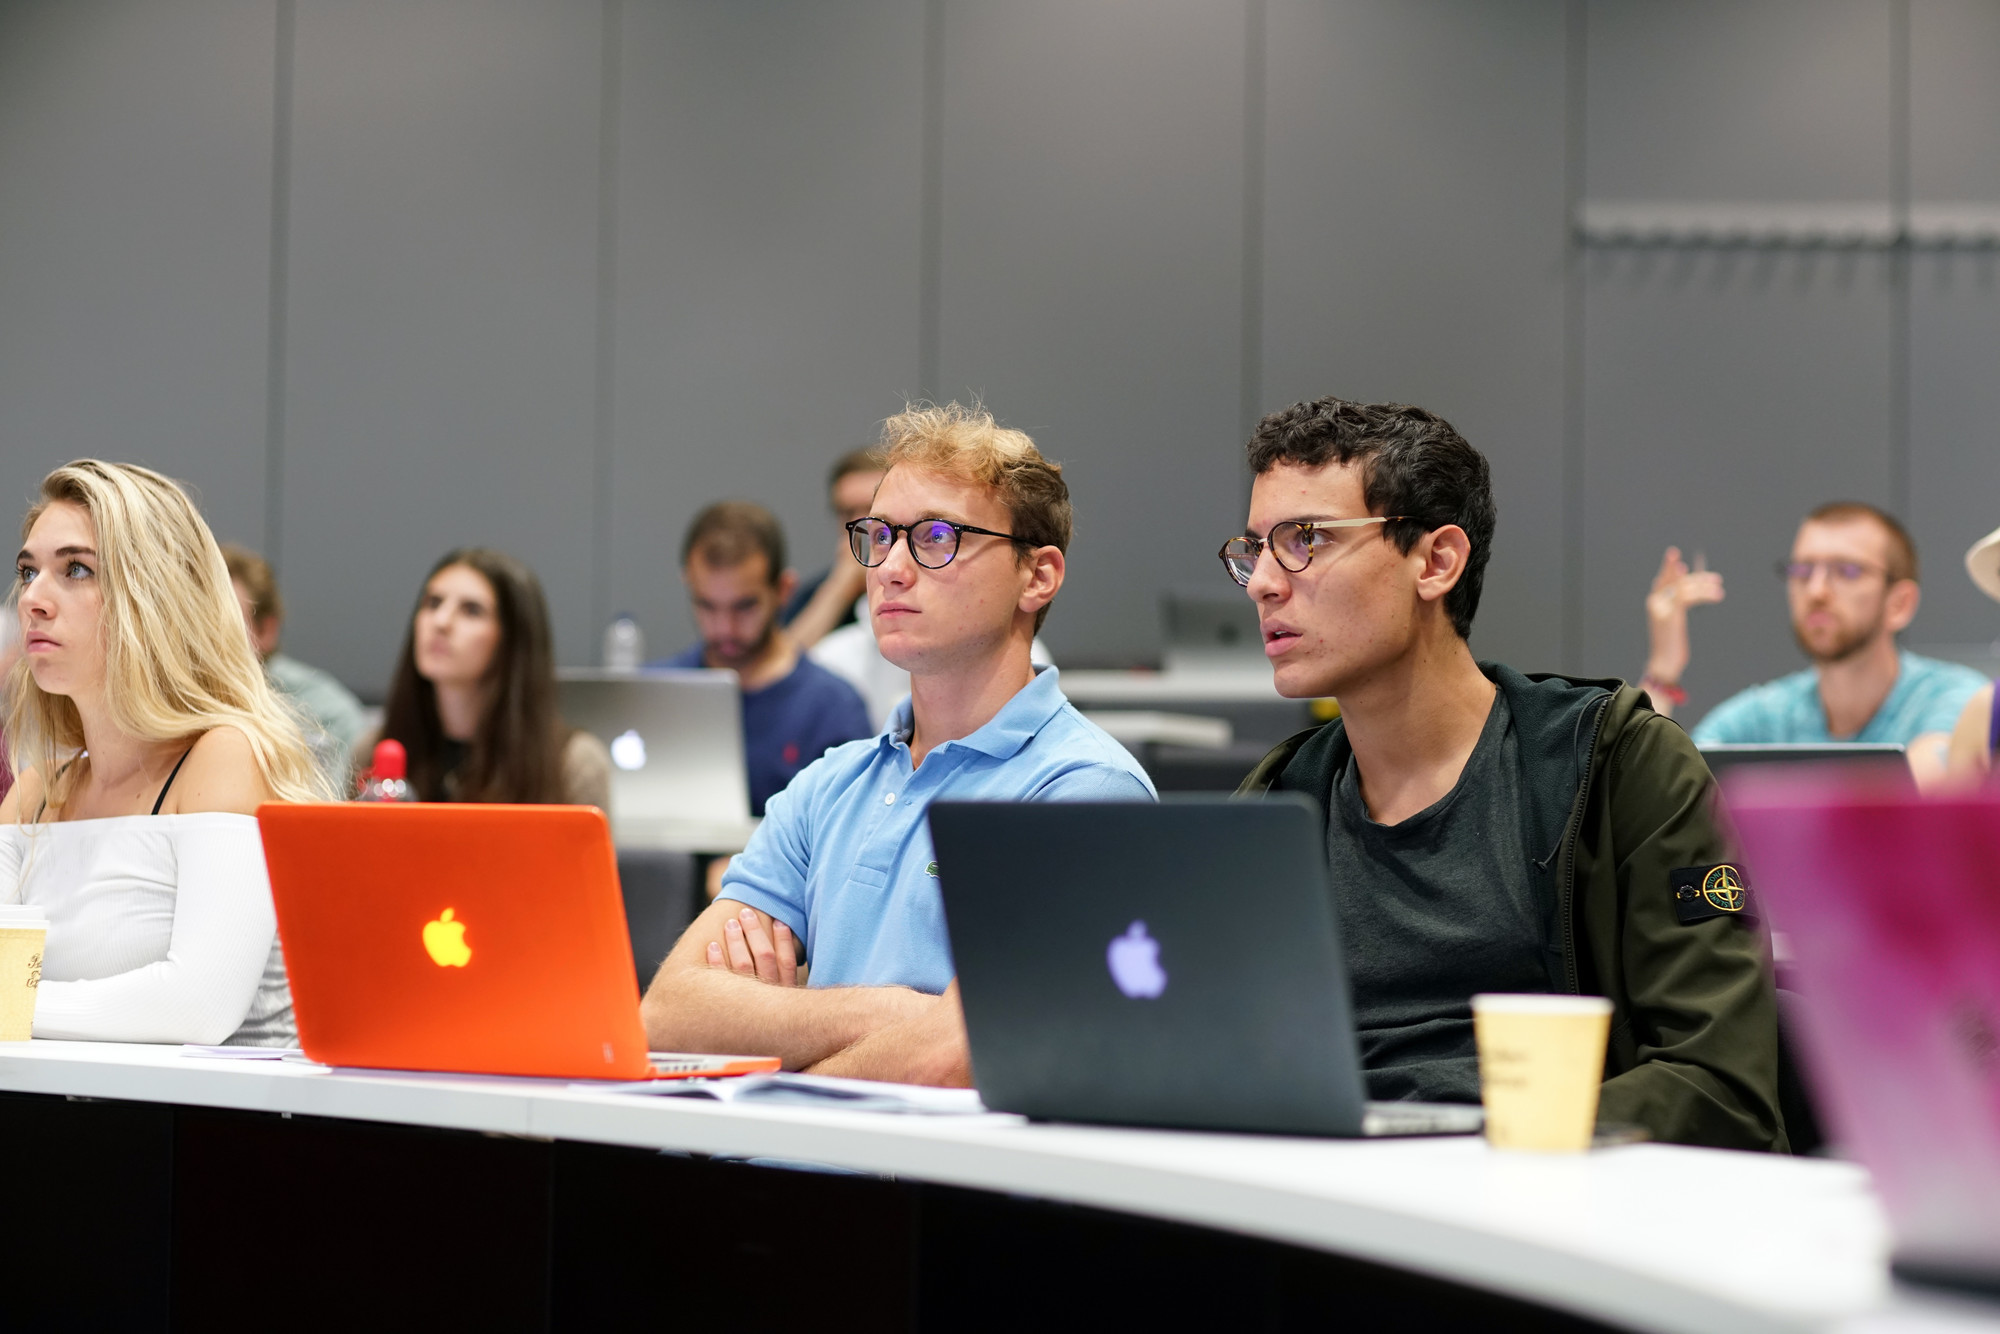
\includegraphics[width=0.495\linewidth]{abt_7295054328859831271Mjc0ODA1Ng.jpg}\hfill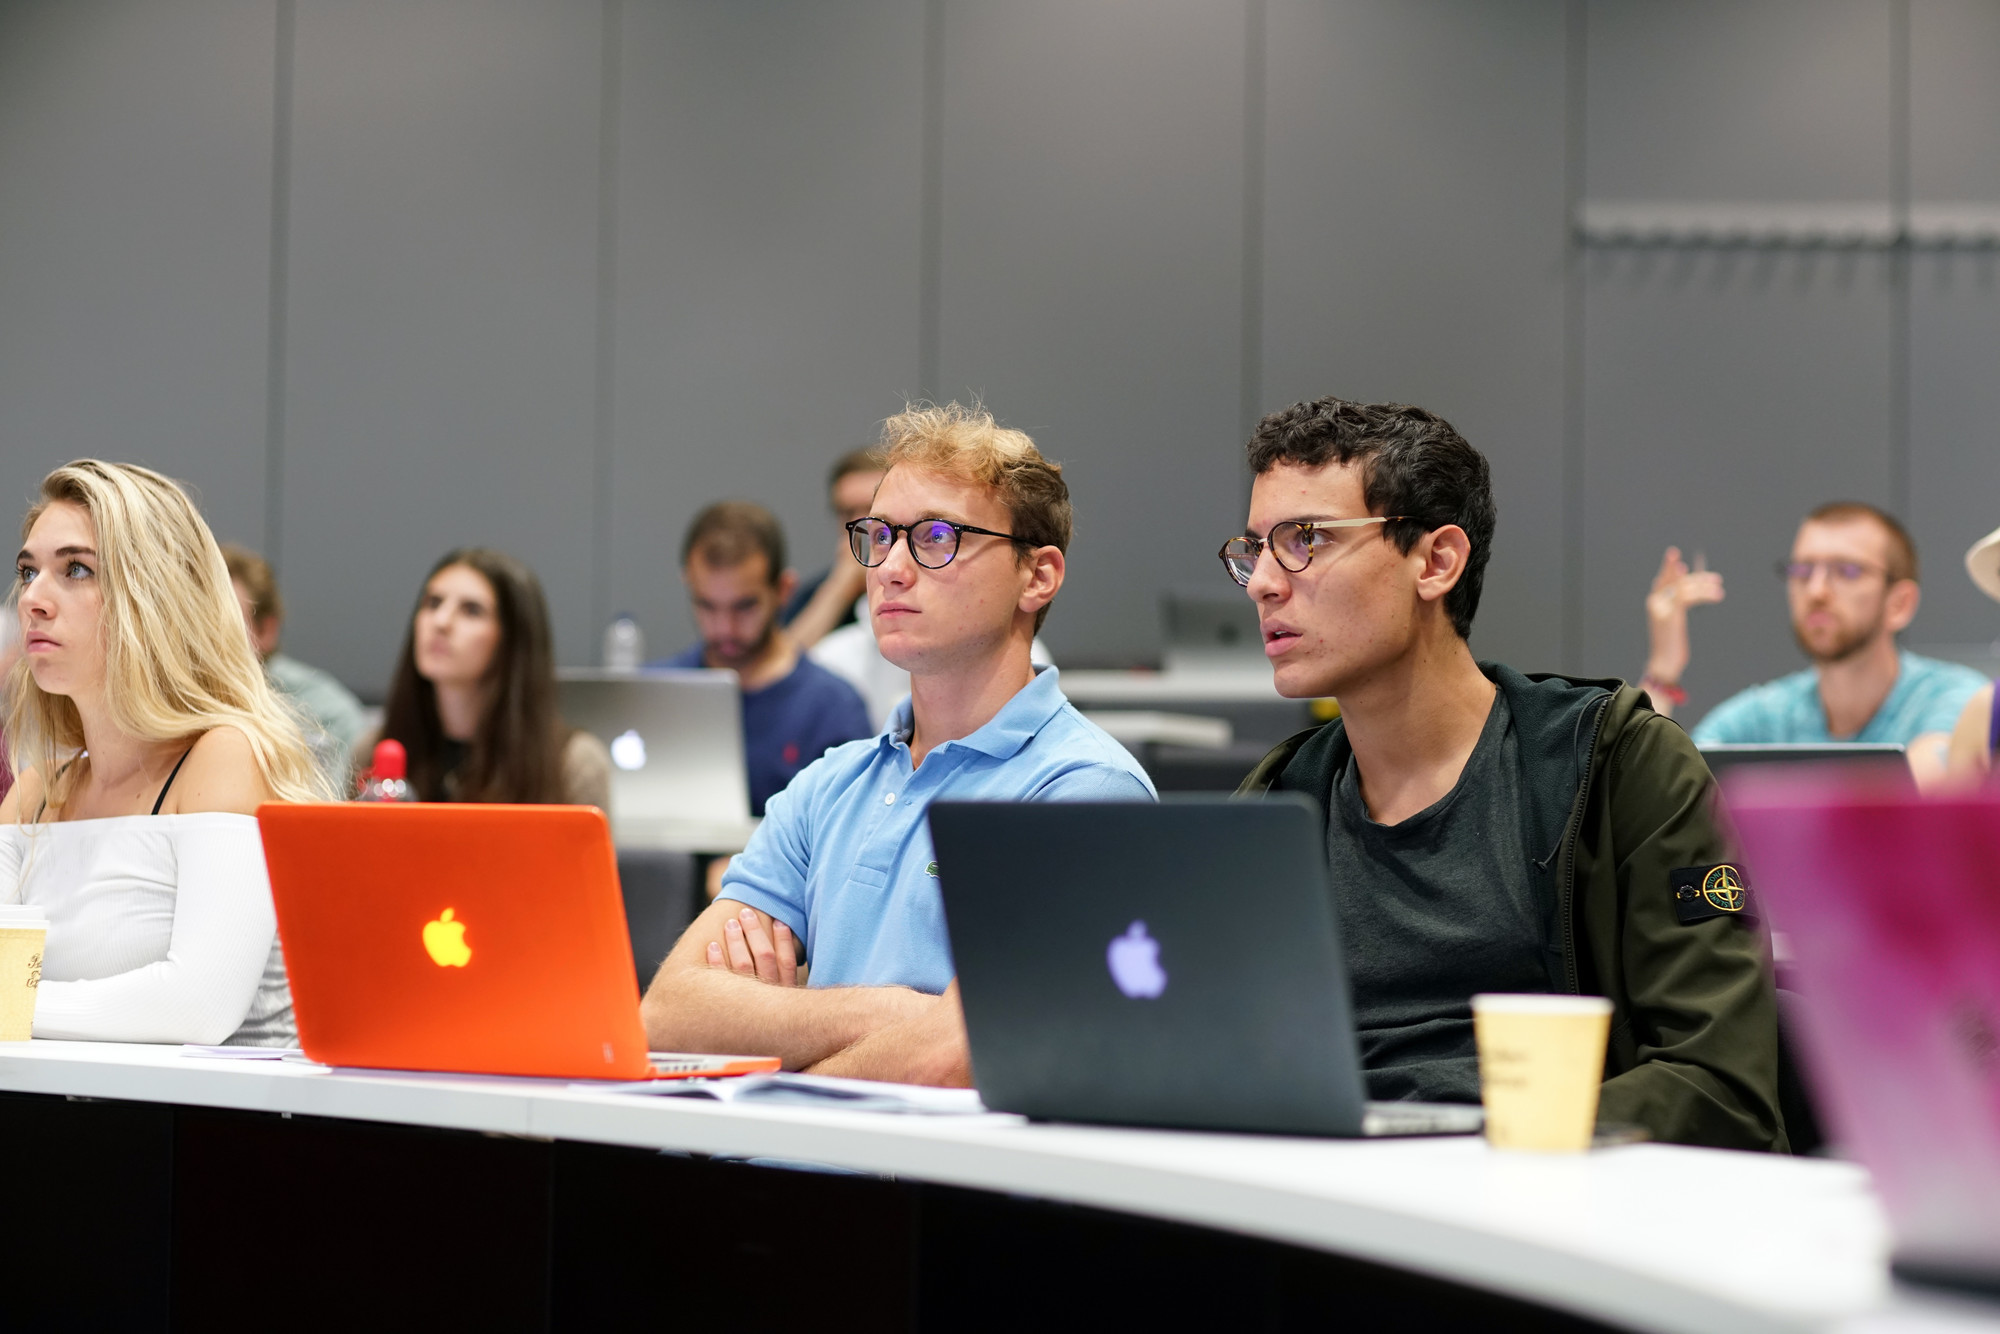
\includegraphics[width=0.495\linewidth]{abt_7295054328859831271Mjc0ODA1Ng.jpg}\par
        \end{column}
    \end{columns}
\end{frame}

%------------------------------------------------

\begingroup
\setbeamercolor{background canvas}{bg=ICLBlue} % Slide background color

\begin{frame}[plain] % 'plain' suppresses the footer
    \medskip % Vertical whitespace
    \centering % Horizontally center the logo
    
\includegraphics[width=0.99\textwidth]{ICL_Logo_White.pdf}
\end{frame}
\endgroup

%------------------------------------------------

\begin{frame}[plain] % 'plain' suppresses the footer
    \medskip % Vertical whitespace
    \centering % Horizontally center the logo
    
\includegraphics[width=0.99\textwidth]{ICL_Logo_Blue.pdf}
\end{frame}

%------------------------------------------------

\begingroup
\setbeamertemplate{background}{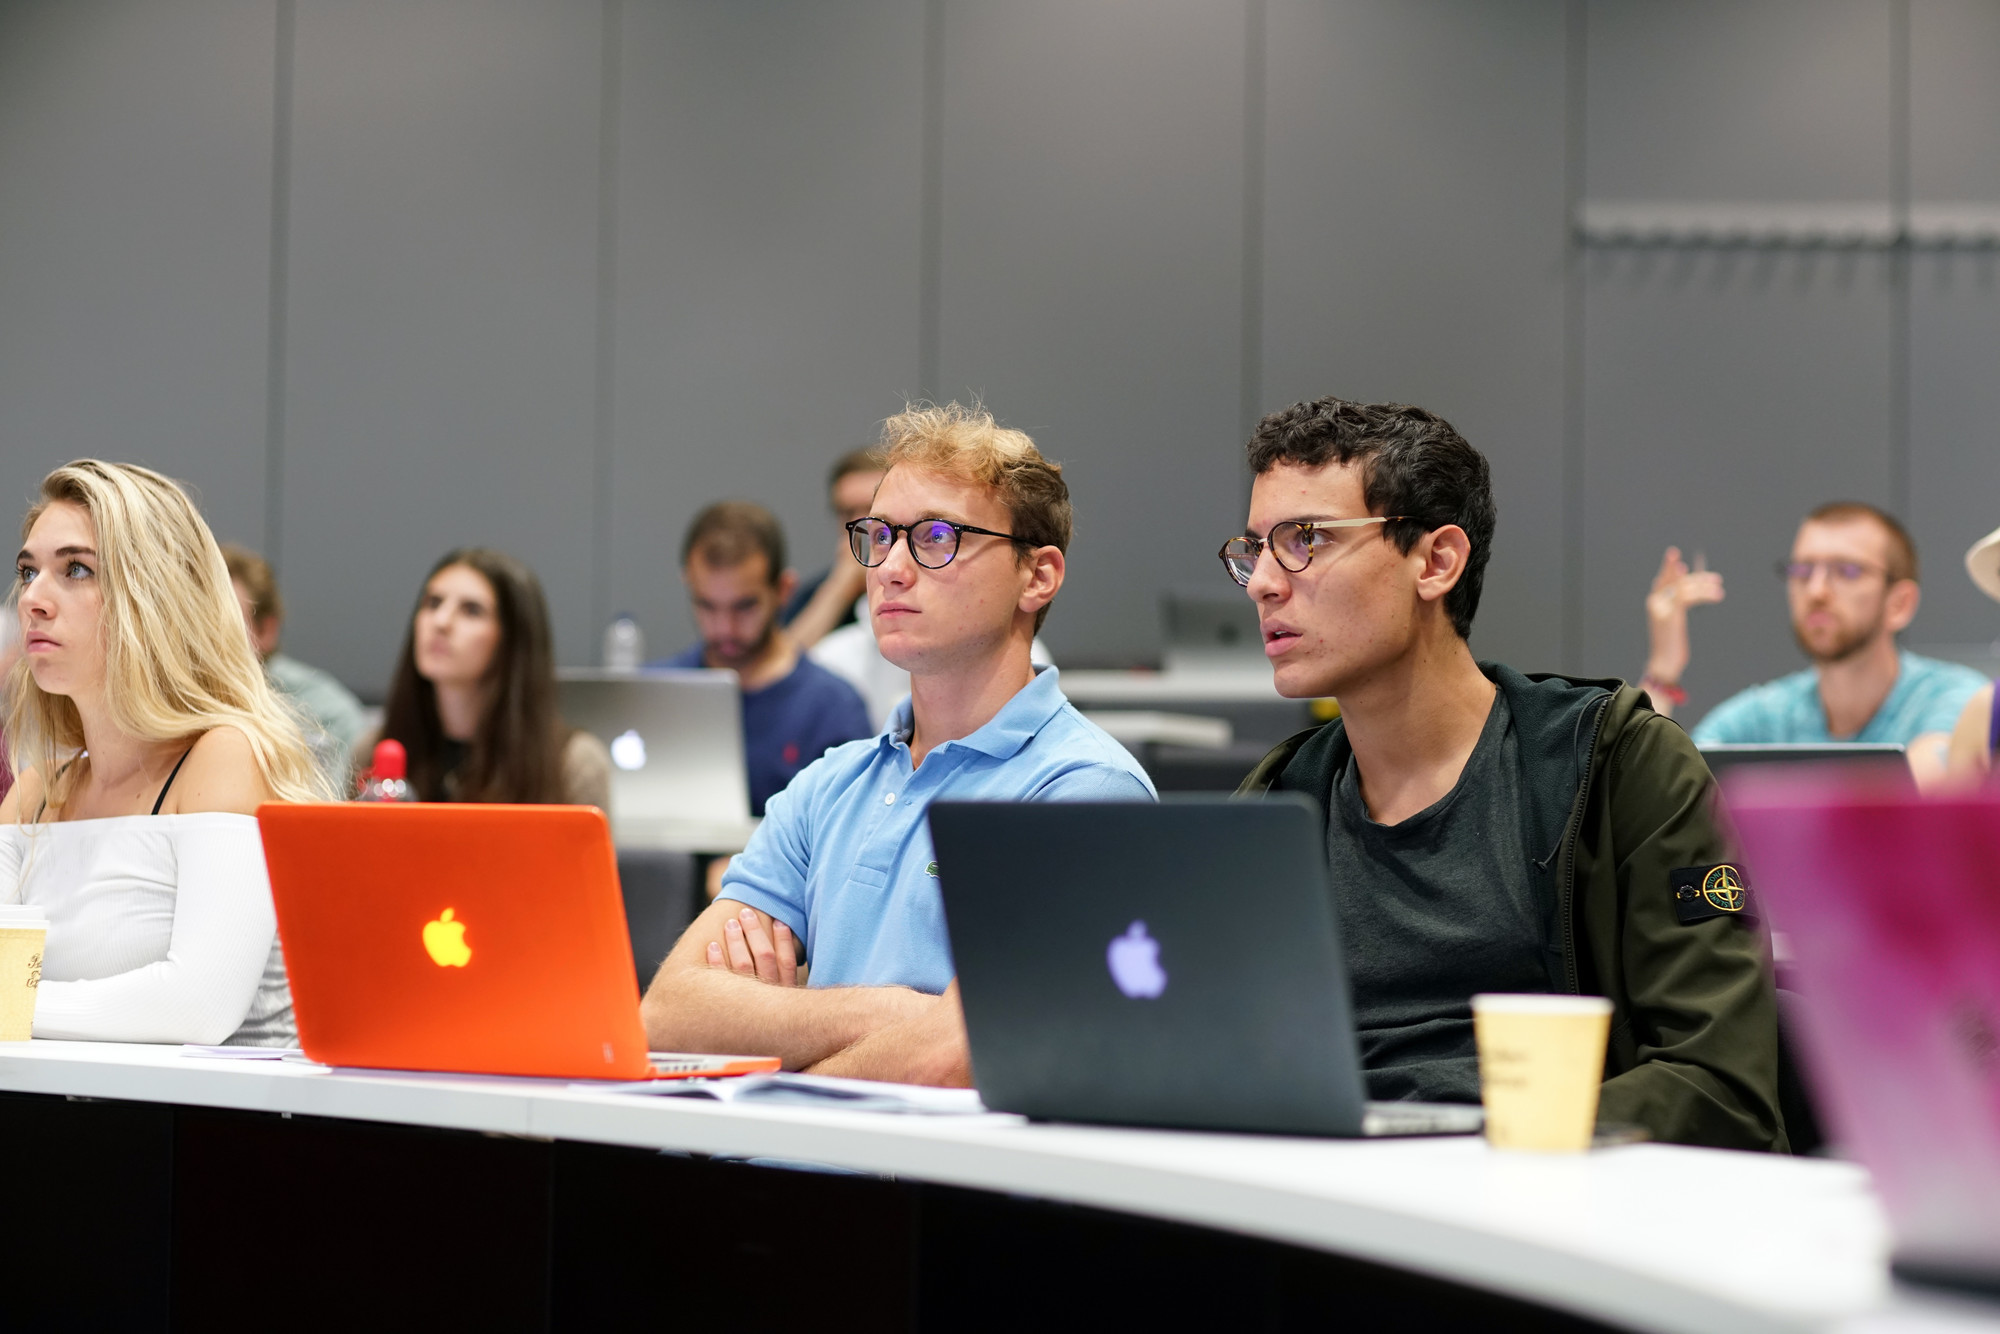
\includegraphics[width=\paperwidth]{abt_7295054328859831271Mjc0ODA1Ng.jpg}} % Slide background image

	\begin{frame}[plain] % 'plain' suppresses the footer
		\medskip % Vertical whitespace
		\centering % Horizontally center the logo
		
\includegraphics[width=0.99\textwidth]{ICL_Logo_White.pdf}
	\end{frame}
\endgroup

%----------------------------------------------------------------------------------------
%	CLOSING SLIDES
%----------------------------------------------------------------------------------------

% Blue closing slide

\begingroup
	\setbeamercolor{background canvas}{bg=ICLBlue} % Slide background color
	\setbeamercolor{normal text}{fg=white}\usebeamercolor[fg]{normal text} % Slide text color
	\setbeamertemplate{closing slide logo}[logo]{ICL_Logo_White.pdf} % Imperial logo color, use 'ICL_Logo_White.pdf' for white and 'ICL_Logo_Blue.pdf' for blue
	\setbeamertemplate{closing slide text}[text]{Thank you} % Slide text
	
	\usebeamertemplate{closing slide} % Output the closing slide
\endgroup

%------------------------------------------------

% White closing slide

\begingroup
	\setbeamercolor{normal text}{fg=ICLBlue}\usebeamercolor[fg]{normal text} % Slide text color
	\setbeamertemplate{closing slide logo}[logo]{ICL_Logo_Blue.pdf} % Imperial logo color, use 'ICL_Logo_White.pdf' for white and 'ICL_Logo_Blue.pdf' for blue
	\setbeamertemplate{closing slide text}[text]{Thank you.\\ Questions?} % Slide text
	
	\usebeamertemplate{closing slide} % Output the closing slide
\endgroup

%----------------------------------------------------------------------------------------

\end{document}
